\documentclass[a4paper,12pt, twoside]{report}
\usepackage[utf8]{inputenc}
\usepackage[T1]{fontenc}
\usepackage[italian]{babel}
\usepackage{amsmath}
\usepackage{amssymb}
\usepackage{titlesec}
\usepackage{multicol}
\usepackage{xcolor}
\usepackage{tikz}
\usetikzlibrary{angles,quotes}
\usepackage{graphicx}
\usepackage{listings}

% Custom template per appunti universita'
\usepackage{noteTemplate}
\newcommand{\CourseTitle}{Sistemi Operativi}
\newcommand{\Author}{Iselle Niccol\`o}


\graphicspath{ {./img/} }

\definecolor{shadecolor}{RGB}{210,210,210}
\newcommand{\defbox}[1]{\noindent\colorbox{shadecolor}
{\parbox{\dimexpr\textwidth-2\fboxsep\relax}{#1}}}

\titleformat{\chapter}
	{\Large\bfseries}		% format
	{}					% label
	{0pt}				% sep
	{\huge}				% before-code

% Authors email
\newcommand{\email}{niccolo.iselle@studenti.univr.it}

\begin{document}
\begin{titlepage}
\centering
\textsc{Universit\`a degli studi di Verona}
\par\vspace{0.5cm}
\rmfamily
Dipartimento di informatica \\
A.A. 2022 - 2023
\par\vspace{1cm}

\includegraphics[scale=0.5]{univr}
\par\vspace{2cm}

\textbf{\Huge{\underline{Sistemi Operativi}}}
\par\vspace{0.5cm}
\textit{\large{-- II Semestre --}}

\par\vspace{1cm}
\footnotesize
Corso tenuto da \\
\normalsize
\textsc{Pravadelli Graziano}
\par\vspace{1cm}
\footnotesize
Appunti a cura di \\
\normalsize
\textsc{Iselle Niccol\`o}
\par\vspace{1cm}

\vfill
\footnotesize
Made with \LaTeX \\
\small
Comunicare eventuali refusi o errori a: \email.
\end{titlepage}
\afterpage{\blankpage}
\tableofcontents

% Rif. lezioni: 6/03/2023 (Deadlock - introduzione);
% 9/03/2023 (Deadlock - prevenzione) e 16/03/2023 (Deadlock - rilevazione e ripristino).
\chapter{Deadlock}

\section{Definizione di deadlock}

In un ambiente con multiprogrammazione, pi\`u thread possono competere per ottenere un numero finito di risorse; se una
risorsa non \`e correntemente disponibile, il thread richiedente passa allo stato d'attesa. In alcuni casi, se le risorse
richieste sono tratenute da altri thread, a loro volta nello stato d'attesa, il thread potrebbe non cambiare pi\`u il suo
stato. Situazioni di questo tipo sono chiamate di \textbf{deadlock} (\emph{stallo}).

\paragraph{\emph{Def}:}
\begin{center}
\defbox{\emph{ciascun processo in un insieme di processi attende un evento che pu\`o essere causato solo da un altro processo dell'insieme}.}
\end{center}


La maggior parte dei sistemi operativi attuali non offre strumenti di prevenzione di queste situazioni, e progettare
programmi che non rischiano lo stallo rimane una responsabilit\`a dei programmatori.

\subsection{Modello di sistema}

Un sistema \`e composto da un numero finito di risorse da distribuire tra pi\`u thread in competizione. Le risorse
possono essere suddivise in tipi differenti, ciascuno formato da un certo numero di istanze identiche. Cicli di CPU,
file e dispositivi di I/O sono tutti esempi di tipi di risorsa.
Anche vari strumenti di sincronizzazione, come i lock mutex e i semafori, sono risorse di sistema e sono una tipica
causa di situazioni di deadlock.

Prima di adoperare una risorsa, un thread deve richiederla e, dopo averla usata deve rilasciarla. Un thread pu\`o
richiedere tutte le risorse necessarie, ma senza mai superare il numero massimo di risorse disponibili nel sistema.
Normalmente un thread pu\`o servirsi di una risorsa soltanto se rispetta la seguente sequenza:
\begin{enumerate}
\item \textbf{Richiesta}: \emph{il thread richiede la risosra e se non \`e disponibile il thread deve attendere finch\'e
non pu\`o acquisire la risorsa}, (\texttt{wait}).
\item \textbf{Uso}: \emph{il thread pu\`o operare sulla risorsa}, (\texttt{ready-queue} o \texttt{cpu}).
\item \textbf{Rilascio}: \emph{il thread rilascia la risorsa}.
\end{enumerate}
La richiesta e il rilascio di risorse avvengono tramite \emph{system call}, ad esempio \texttt{open()} e \texttt{close()} su un file.

\subsection{Condizioni necessarie}

Si pu\`o avere una situazione di deadlock se e solo se in un sistema si verificano \emph{contemporaneamente} le seguenti condizioni:
\begin{center}
\defbox{
\begin{enumerate}
\item \textbf{Mutua esclusione}: \emph{almeno una risorsa deve essere non condivisibile}.
\item \textbf{Hold \& Wait}: \emph{deve esistere un processo che detiene una risorsa e che attende di acquisirne un'altra,
detenuta da un altro processo}.
\item \textbf{No preemption}: \emph{Le risorse non possono essere rilasciate se non ``volontariamente'' dal processo che le detiene}.
\item \textbf{Attesa circolare}: \emph{Deve esistere un insieme di processi che attendono ciclicamente il liberarsi di una risorsa}.
\end{enumerate}
}
\end{center}

Possiamo notare che la condizione dell'attesa circolare implica la condizione di hold \& wait, quindi le quattro condizioni
non sono completamente indipendenti.

\subsection{Esempio di deadlock}

\begin{center}
\defbox{
\begin{itemize}
\item P e Q devono utilizzare A e B in modo esclusivo
\end{itemize}
\begin{tikzpicture}
\node at (0,0) {};
% riquadro 1 - processo P
\draw (2,0) -- (2,4);
\draw (2,0) -- (5,0);
\draw (5,0) -- (5,4);
\draw (5,4) -- (2,4);
\node at (2,4) [below right] {Processo P};
\node at (2,3.2) [right][red] {get A};
\node at (2,2.8) [below right] {$\dots$};
\node at (2,2.3) [right][blue] {get B};
\node at (2,2) [below right] {$\dots$};
\node at (2,1.4) [right][red] {release A};
\node at (2, 1) [below right] {$\dots$};
\node at (2, 0.4) [right][blue] {release B};

% Freccie
\draw[->][line width=0.7][orange] (3.25, 3.2) -- (7.85, 2.3); 
\draw[->][line width=0.7][teal] (7.85,3.2) -- (3.25, 2.3);

% riquadro 2 - process Q
\draw (8,0) -- (8,4);
\draw (8,0) -- (11,0);
\draw (11,0) -- (11,4);
\draw (11,4) -- (8,4);
\node at (8,4) [below right] {Processo Q};
\node at (8,3.2) [right][blue] {get B};
\node at (8,2.8) [below right] {$\dots$};
\node at (8,2.3) [right][red] {get A};
\node at (8,2) [below right] {$\dots$};
\node at (8,1.4) [right][blue] {release B};
\node at (8, 1) [below right] {$\dots$};
\node at (8, 0.4) [right][red] {release A};
\end{tikzpicture}
}
\end{center}

In questo caso ci sono sei possibili sequenze di richiesta/rilascio. Il deadlock dipende quindi dalla dinamica dell'esecuzione,
comse possiamo vedere nel grafico:

\begin{center}
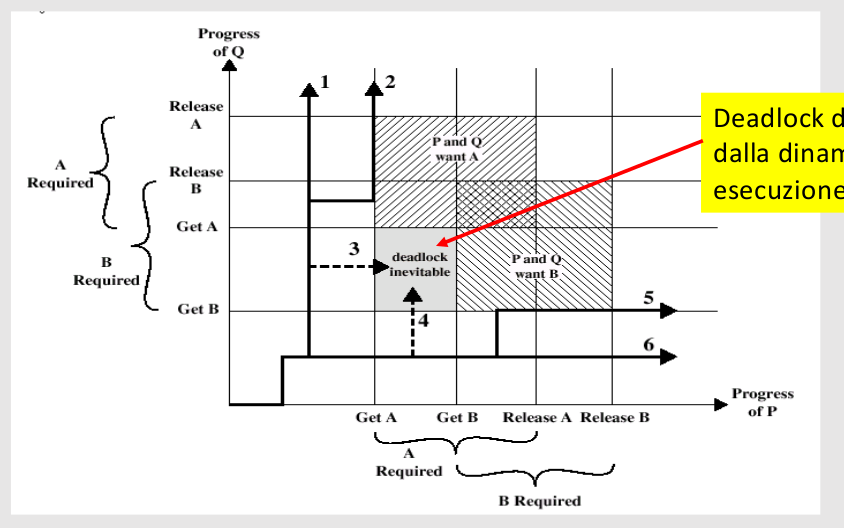
\includegraphics[scale=0.35] {graf}
\end{center}

\section{RAG: Resource Allocation Graph}

Le situazioni di stallo si possono descrivere con maggior precisione avvalendosi di una rappresentazione detta \emph{grafo
di assegnazione delle risorse}. Si tratta di un insieme di nodi ($V$) e archi ($E$), con l'insieme di vertici V composto
da due sottoinsiemi: i processi e le risorse. Un arco diretto dal processo $P_i$ alla risorsa $R_j$ ($P_i \to R_j$) significa
che il processo ha richiesto un'istanza della risorsa, ed \`e attualmente in attesa di essa. Un arco diretto da un'istanza
della risorsa $R_j$ verso il processo $P_i$ sta ad indicare che il processo detiene quella risorsa.

Graficamente un processo si rappresenta con un cerchio e le risorse si rappresentano con un rettangolo. Siccome il tipo
di risorsa $R_j$ pu\`o avere pi\`u istanze, queste si rappresentano con dei pallini all'interno del rettangolo $R_j$.

\subsection{Esempio di RAG}

\begin{tikzpicture}
% Primo riquadro
\node at (0,5) [below right][red] {1};
\draw (0,0) -- (0,5);
\draw (0,0) -- (3,0);
\draw (0,5) -- (3,5);
\draw(3,0) -- (3,5);
\filldraw[color=black, fill=white] (1.5, 4) circle (0.3);
\node at (1.5, 4) {$P_1$};
\node at (3.25,0) [below] {Request $\rightarrow$};

\draw (1, 2.25) rectangle ++(1,0.75) node[below right]{$R_1$};
\filldraw[color=black, fill=white] (1.5, 2.5)  circle (0.1);
\filldraw[color=black, fill=white] (1.25, 2.75)  circle (0.1);
\filldraw[color=black, fill=white] (1.75, 2.75)  circle (0.1);
\draw[->] (1.5,2.4) -- (1.5,1.3);
\filldraw[color=black, fill=white] (1.5,1) circle (0.3);
\node at (1.5, 1) {$P_2$};

% Secondo riquadro
\node at (3.5,5) [below right][red] {2};
\draw (3.5,0) -- (3.5,5);
\draw (3.5,0) -- (6.5,0);
\draw (3.5,5) -- (6.5,5);
\draw(6.5,0) -- (6.5,5);
\filldraw[color=black, fill=white] (5, 4) circle (0.3);
\node at (5, 4) {$P_1$};
\node at (6.75,0) [below] {Acquisition $\rightarrow$};

\draw (4.5, 2.25) rectangle ++(1,0.75) node[below right]{$R_1$};
\filldraw[color=black, fill=white] (5, 2.5)  circle (0.1);
\filldraw[color=black, fill=white] (4.75, 2.75)  circle (0.1);
\filldraw[color=black, fill=white] (5.25, 2.75)  circle (0.1);
\draw[->] (5,2.4) -- (5,1.3);
\draw[->] (4.8,3.7) -- (4.8,3);
\draw[->] (5.2,3.7) -- (5.2,3);

\filldraw[color=black, fill=white] (5,1) circle (0.3);
\node at (5, 1) {$P_2$};

% Terzo riquadro
\node at (7,5) [below right][red] {3};
\draw (7,0) -- (7,5);
\draw (7,0) -- (10,0);
\draw (7,5) -- (10,5);
\draw(10,0) -- (10,5);
\filldraw[color=black, fill=white] (8.5, 4) circle (0.3);
\node at (8.5, 4) {$P_1$};
\node at (10.75,0) [below] {Release $\rightarrow$};

\draw (8, 2.25) rectangle ++(1,0.75) node[below right]{$R_1$};
\filldraw[color=black, fill=white] (8.5, 2.5)  circle (0.1);
\filldraw[color=black, fill=white] (8.25, 2.75)  circle (0.1);
\filldraw[color=black, fill=white] (8.75, 2.75)  circle (0.1);
\draw[->] (8.5,2.4) -- (8.5,1.3);
\draw[->] (8.25,2.85) -- (8.4,3.7);
\draw[->] (8.7,2.85) -- (8.6,3.7);

\filldraw[color=black, fill=white] (8.5,1) circle (0.3);
\node at (8.5, 1) {$P_2$};

% Quarto riquadro
\node at (10.5,5) [below right][red] {4};
\draw (10.5,0) -- (10.5,5);
\draw (10.5,0) -- (13.5,0);
\draw (10.5,5) -- (13.5,5);
\draw(13.5,0) -- (13.5,5);
\filldraw[color=black, fill=white] (12, 4) circle (0.3);
\node at (12, 4) {$P_1$};

\draw (11.5, 2.25) rectangle ++(1,0.75) node[below right]{$R_1$};
\filldraw[color=black, fill=white] (12, 2.5)  circle (0.1);
\filldraw[color=black, fill=white] (12.25, 2.75)  circle (0.1);
\filldraw[color=black, fill=white] (11.75, 2.75)  circle (0.1);
\draw[->] (12,2.4) -- (12,1.3);
\draw[->] (12.2,2.85) -- (12.1,3.7);

\filldraw[color=black, fill=white] (12,1) circle (0.3);
\node at (12, 1) {$P_2$};

\draw (3,-1) -- (10.5,-1);
\draw (3,-1) -- (3,-3);
\draw (3,-3) -- (10.5,-3);
\draw (10.5, -1) -- (10.5, -3);
\node at (6.1,-1.5) {$\cdot$ \texttt{V = \{\{P$_1$, P$_2$\}, \{R$_1$\}\}}};
\node at (6.0, -2) {$\cdot$ \texttt{E$_{iniziale}$ = \{(R$_1$, P$_2$)\}}};
\node at (6.95, -2.5){$\cdot$ \texttt{E$_{finale}$ = \{(R$_1$, P$_1$), (R$_2$, P$_2$)\}}};

\end{tikzpicture}
\begin{enumerate}
\item Nel primo riquadro della figura abbiamo che $P_1$ non sta usando la risorsa $R_1$, mentre il processo $P_2$
detiene un'istanza della risorsa $R_1$. Nessuno dei due processi \`e in attesa.
\item Il processo $P_1$ fa una richiesta per usare le due istanze libere della risorsa $R_1$. In questo contesto $P_2$
detiene una risorsa e potrebbe essere in esecuzione oppure nella \emph{ready queue}. Il processo $P_1$ invece sar\`a
sicuramente in \emph{attesa}, sta aspettando che il sistema operativo conceda le risorse richieste.
\item Il sistema operativo ha concesso le due istanze di $R_1$ libere al processo $P_1$, che non \`e pi\`u in attesa ma
potrebbe essere nello stato pronto o in esecuzione, cosi come il processo $P_2$.
\item Nell'ultimo schema il processo $P_1$ ha rilasciato un'istanza della risorsa $R_1$, entrambi i processi sono nello
stato pronto oppure (solo uno alla volta) in esecuzione.
\end{enumerate}

\newpage
\`E possibile individuare un eventuale deadlock attraverso il RAG: ci sono tre possibili casi.
\begin{itemize} 
\item Se non sono presenti cicli, non ci sono deadlock.
\item Se \`e presente un ciclo e le risorse sono presenti in un'unica istanza, siamo sicuramente in deadlock.
\begin{center}
\begin{tikzpicture}
\filldraw[color=black, fill=white] (1,1) circle (0.2);
\draw[->](1,1.2) -- (1,1.75);
\draw (0.75, 1.75) rectangle ++(0.5,0.5);
\draw[->](1,2.25) -- (1,2.78);
\filldraw[color=black, fill=white] (1,3) circle (0.2);
\draw[->](1.2,3) -- (1.75,3);
\draw (1.75, 2.75) rectangle ++(0.5,0.5);
\draw[->](2.25,3) -- (2.78,3);
\filldraw[color=black, fill=white] (3,1) circle (0.2);
\draw[->](3,2.78) -- (3,2.25);
\draw (1.75, 0.75) rectangle ++(0.5,0.5);
\draw[->](3,1.75) -- (3,1.2);
\filldraw[color=black, fill=white] (3,3) circle (0.2);
\draw[->](2.78,1) -- (2.25,1);
\draw (2.75, 1.75) rectangle ++(0.5,0.5);
\draw[->](1.75,1) -- (1.2,1);
\node at (2, 0) [red] {\textbf{DEADLOCK}};
\end{tikzpicture}
\end{center}
\item Se \`e presente un ciclo ma le risorse hanno pi\`u istanze ciascuna, potrebbe non esserci un deadlock, dipende dallo
schema di allocazione.
\begin{center}
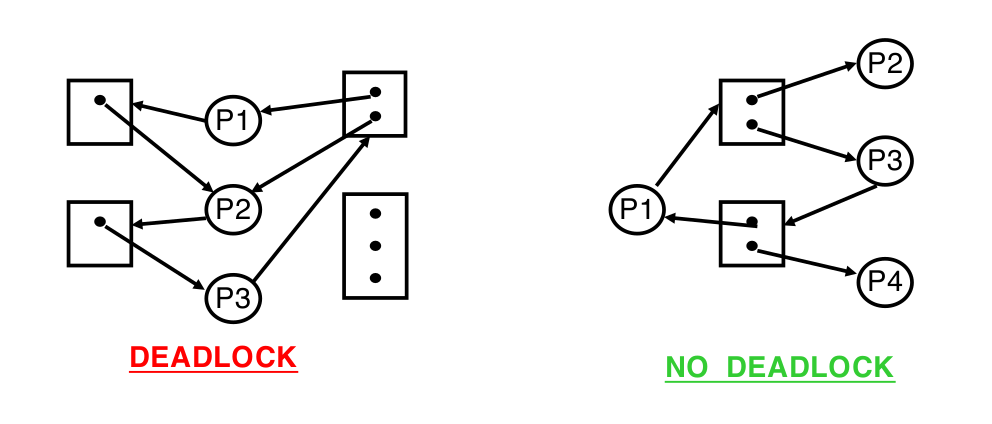
\includegraphics[scale=0.3]{ciclograf}
\end{center}
\end{itemize}

\section{Gestione dei deadlock}
Il problema del deadlock si pu\`o affrontare in vari modi che comportano uno spreco di risorse pi\`u o meno elevato. 

\paragraph{Prevenzione statica:}
evitare che si possa verificare una delle quattro condizioni di stallo, ad esempio negando le risorse ad un processo
istanze di risorse libere che potrebbero portare ad una situazione di possibile deadlock.

\paragraph{Prevenzione dinamica:}
detta \emph{avoidance}, \`e basata sull'allocazione delle risorse ma non \`e mai usata poich\'e richiede una conoscenza
troppo approfondita delle richieste di risorse.

\paragraph{Rivelazione e ripristino:}
chiamata anche \emph{detection and recovery}, permette che si verifichino dei deadlock ma, quando ci\`o avviene, utilizza
metodi di ripristino per portare il sistema al funzionamento normale.

\paragraph{Algoritmo dello struzzo:}
vista la rarit\`a degli eventi di stallo e il costo elevato per la loro gestione, si pu\`o scegliere di non fare nulla.
Eventualmente in alcuni casi, se si verifica una situazione di stallo, sar\`a necessario riavviare il calcolatore. In
questo caso non si ha uno spreco di risorse. Naturalmente non \`e utilizzabile in sistemi \emph{saefty critical}.

\subsection{Prevenzione statica}

Impone una regola a prescindere dall'esecuzione del sistema. L'obbiettivo \`e di impedire che si verifichi una delle
quattro condizioni necessarie per il verificarsi di un deadlock.

\subsubsection{Mutua esclusione}
Per eliminare la \emph{mutua esclusione} almeno una risorsa deve essere non condivisibile; ma poich\'e per alcune risorse
la mutua esclusione \`e irrinunciabile, non si possono prevenire in generale le situazioni di stallo negando questa condizione.
Inoltre, rimuovendola si avrebbe il rischio di una \emph{race condition}, peggiorando la situazione.

\subsubsection{Hold and wait}
Per assicurare che la condizione di \emph{hold and wait} non si presenti mai nel sistema, occorre garantire che un
processo allochi prima dell'esecuzione tutte le risorse che deve utilizzare oppure che possa ottenere una risorsa solo se
non ne ha altre. A causa della natura dinamica della richiesta di risorse questa condizione presenta alcuni problemi: un
basso utilizzo di risorse, perch\'e potrebbero rimanere assegnate per lunghi periodi tempo ad un processo che necessita
di usarle per un breve periodo, e perch\'e si presenta il rischio di \emph{starvation} per risorse molto popolari richieste
da numerosi processi.

Un ulteriore problematica per l'attuazione di questi protocolli \`e la necessit\`a di sapere tutte le risorse richieste
dal processo prima dell'esecuzione dello stesso.

\subsubsection{Assenza di prelazione}
Per assicurare che questa condizione non sussista, si pu\`o impiegare il seguente protocollo. Se un processo che detiene
una o pi\`u risorse ne richiede un'altra che non gli si pu\`o assegnare immediatamente, allora si esercita la prelazione
su tutte le risorse detenute dal processo. Si ha cio\`e il rilascio implicito di queste risorse e il processo esce dallo
stato di attesa solo quando pu\`o ottenere sia le vecchie risorse che quella nuova che sta richiedendo.

Un altro sistema \`e quello di verificare la disponibilit\`a delle risorse richieste: se sono disponibili vengono assegnate,
se non lo sono, si verifica se sono assegnate ad un processo in attesa. In tal caso si prelazionano dal processo in attesa
e si assegnano al richiedente. Se le risorse non sono disponibili n\'e sono possedute da un processo in attesa, il
richiedente viene messo in attesa. Un processo si pu\`o avviare nuovamente solamente quando riceve tutte le risorse
richieste e quelle eventualmente prelazionate mentre era in attesa.

Questo protocollo \`e applicato spesso per risorse il cui stato si pu\`o facilmente salvare e recuperare, mentre non si
pu\`o appilcare in generale a risorse come mutex o semafori.

\subsubsection{Attesa circolare}

Le tre precedenti condizioni sono generalmente difficili da evitare nella maggior parte delle situazioni. Tuttavia,
l'\emph{attesa circolare} offre un'opportunit\`a per una soluzione pratica che renda non valida una delle condizioni di
deadlock. Un metodo per evitare l'attesa circolare consiste nell'imporre un ordinamento totale all'insieme di tutti i
tipi di risorse e imporre che ciascun processo richieda le risorse in ordine crescente. Ovvero, assegnamo una priorit\`a
ad ogni risorsa:
\[ F: R \to \mathbb{N} \]
\[ F(R_0) < F(R_1) < \dots < F(R_n) \]
Un processo pu\`o richiedere risorse solo in ordine crescente di priorit\`a, quindi l'attesa circolare diventa impossibile poich\`e:
\begin{itemize}
\item Se $P_0 \to R_0 \to P_1 \to \dots \to R_{n-1} \to P_n \to R_n \to P_0$
\item allora, $F(R_0) < F(R_1) < \dots < F(R_n) < F(R_0)$, impossibile.
\end{itemize}
Con questo sistema se un processo $P_i$ che detiene le risorse $R_1$, $R_3$ ed $R_6$ richiede la risorsa $R_4$, non pu\`o
ottenerla e deve cedere tutte le risorse che detiene, cosi da richiderle in seguito nel corretto ordine. Se sono necessarie
pi\`u istanze dello stesso tipo di risorsa si deve presentare una singola richiesta per tutte le istanze.

\subsection{Prevenzione dinamica}

Le tecniche di prevenzione statica possono portare ad un basso utilizzo delle risorse perch\`e mettono vincoli sul modo
in cui i processi possono accedere alle risorse. Un diverso approccio \`e quello della \emph{prevenzione dinamica}. In
questo contesto potranno esserci ancora situazioni in cui alcuni processi si vedranno negate delle risorse, ma si tratta
di una valutazione caso per caso. Tuttavia, queste tecniche di prevenzione dinamica non sono \emph{ragionevolmente
implementabili} in sistemi general puprose perch\'e, per poter effettuare le analisi sulle richieste di risorse il sistema
dovrebbe avere una conoscenza del futuro. Questo tipo di prevenzione \`e possibile farlo in alcune situazioni \emph{application specific}.

I requisiti necessari per l'implementazione di questa tecnica di prevenzione sono la conoscenza delle risorsi disponibili,
facilmente ottenibile perch\`e il sistema ha una quantit\`a di risorse finite; la conoscenza del \emph{caso peggiore} ovvero
il numero massimo di risorse richieste da ogni processo durante l'esecuzione, molto pi\`u difficile da calcolare. Infine, \`e
necessario sapere lo stato corrente del sistema, per determinare se la concessione di risorse, a fronte di una richiesta,
possa portare il sistema in uno \emph{stato unsafe}.

\subsection{Stato safe, unsafe e deadlock}

\paragraph{\emph{Def}:}
\begin{center}
\defbox{\emph{Un sistema si trova in uno \textbf{stato safe} se esiste una sequenza safe, ovvero se usando le risorse
disponibili, pu\`o allocare risorse ad ogni processo, in qualche ordine, in modo che ciascuno di essi possa terminare la sua esecuzione}.}
\end{center}

Una sequenza di processi $\langle P_1, P_2, \dots, P_n \rangle$ \`e una sequenza sicura per lo stato di assegnazione attuale se, per ogni $P_i$, le richieste che il processo $P_i$ pu\`o ancora fare si possono soddisfare impiegando le risorse attualmente disponibili pi\`u le risorse possedute da tutti i processi $P_j$ con $j < i$. In questa situazione, se le risorse necessarie al processo $P_i$ non sono disponibili immediatamente, quest'ultimo attender\`a che tutti i processi $P_j$ abbiano finito, a quel punto potr\`a ottenere tutte le risorse necessarie e terminare. Se non esiste una sequenza di questo tipo, lo stato del sistema si dice \emph{unsafe}.
Si noti che uno stato \emph{sicuro} non porter\`a ad uno stallo. Viceversa, quando si ha un deadlock, sicuramente il sistema \`e in uno stato \emph{non sicuro}; tuttavia non tutti gli stati unsafe sono stati di deadlock.

\subsubsection{Spazio degli stati}

\begin{center}
\begin{tikzpicture}
\filldraw[color=black, fill=lightgray!40] (0,0) rectangle ++(8,8);
\filldraw[color=black, fill=white] (1,6) rectangle ++(2.6,1.35);
\filldraw[color=black, fill=lightgray] (0,5) -- (8,6) -- (8,0) -- (0,0) -- (0,5);

\node at (2.3, 6.65) {\textbf{deadlock}};
\node at (6.8,7.3) {\textbf{unsafe}};
\node at (7,5.25) {\textbf{safe}};
\end{tikzpicture}
\end{center}

\subsubsection{Esempi di stato safe e unsafe}
\begin{multicols}{2}[
Supponiamo di avere 3 processi, $P_0$, $P_1$, $P_2$, e 12 istanze di una risorsa di cui 3 sono libere. Siamo in uno stato Safe?]
\begin{center}
\begin{tabular} {| c | c | c |}
\hline
& Richieste & Possedute \\
\hline
\hline
$P_0$ & 10 & 5 \\
$P_1$ & 4 & 2 \\
$P_2$ & 9 & 2 \\
\hline
\end{tabular}
\end{center}

Si, esiste una sequenza safe $\langle P_1, P_0, P_2 \rangle$ tale per cui tutti i processi possono terminare.
\end{multicols}
\begin{multicols}{2}[
Se ora $P_2$ richiede 1 risorsa e gli viene assegnata, siamo ancora in uno stato safe?]
\begin{center}
\begin{tabular} {| c | c | c |}
\hline
& Richieste & Possedute \\
\hline
\hline
$P_0$ & 10 & 5 \\
$P_1$ & 4 & 2 \\
$P_2$ & 9 & 3 \\
 \hline
\end{tabular}
\end{center}
Non siamo pi\`u in uno stato safe. Con le restanti 2 risorse $P_1$ pu\`o eseguire, ma quando termina libera solo 4 risorse: a $P_0$ ne servono 5 e a $P_2$ ne servono 6. Deadlock $P_2 \leftrightarrow P_0$.
\end{multicols}


\subsubsection{Deadlock \& Risorse}

Nel caso della prevenzione il costo \`e dato da un basso utilizzo delle risorse. Infatti, in alcuni casi delle risorsi disponibili non vengono concesse ai processi per evitare che il sistema entri in uno stato non sicuro.

Con le tecniche di rilevazione e ripristino il sistema concede risorse fino alla massima disponibilit\`a, ma ogni tanto devono sprecare tempo per verificare se si \`e verificata una situazione di deadlock e, in caso affermativo attuare il recovery e quindi sprecare altro tempo per ritornare ad uno stato precedente.

La prevenzione, che si divide in \emph{statica} e \emph{dinamica}, \`e necessaria nei sistemi \emph{saefty critical}; le soluzioni di detection \& recovery, invece, funzionano in tutte quelle situazioni in cui il deadlock, se avviene, non \`e catastrofico.

\section{Algoritmi per la prevenzione dinamica}

Per implementare la \emph{prevenzione dinamica} abbiamo due alternative. La prima prevede l'utilizzo di un algoritmo con RAG, ma funziona solo se c'\`e una sola istanza per risorsa. La seconda alternativa usa l'\emph{algoritmo del banchiere}, che ha il vantaggio di funzionare con qualsiasi numero di istanze di risorse, ma \`e pi\`u complicato.

\subsection{Algoritmo con RAG}

Questo algoritmo prevede di aggiungere ai \emph{resource allocation graph} un nuovo tipo di arco: l'arco di \emph{richiesta} (\emph{claim edge}). Otteniamo quindi tre tipi di archi:
\begin{itemize}
\item \textcolor{blue}{\underline{\emph{Arco di richiesta}}}: va dal processo $P_i$ alla risorsa $R_j$ e si indica con una freccia piena, il processo \`e in attesa di ottenere una istanza di quella risorsa.
\begin{center}
\begin{tikzpicture}
\filldraw[color=black, fill=white] (2,0.5) rectangle ++(1,1);
\node at (2.5,1) {$R_j$};
\draw[->][thick][blue] (-0.5,1) -- (2,1);
\filldraw[color=black, fill=white] (-1,1) circle (0.5);
\node at (-1,1) {$P_i$};
\end{tikzpicture}
\end{center}
\item \textcolor{red}{\underline{\emph{Arco di possesso}}}: va dalla risorsa $R_j$ al processo $P_i$ che la detiene. Si indica con una freccia piena.
\begin{center}
\begin{tikzpicture}
\filldraw[color=black, fill=white] (2,0.5) rectangle ++(1,1);
\node at (2.5,1) {$R_j$};
\draw[->][thick][red] (2,1) -- (-0.5,1) ;
\filldraw[color=black, fill=white] (-1,1) circle (0.5);
\node at (-1,1) {$P_i$};
\end{tikzpicture}
\end{center}
\item \textcolor{teal}{\underline{\emph{Arco di reclamo}}}: si indica con una freccia tratteggiata che va dal processo $P_i$ alla risorsa $R_j$. Significare che in un qualche momento futuro, il processo $P_i$ vorr\`a una istanza della risorsa $R_j$.
\begin{center}
\begin{tikzpicture}
\filldraw[color=black, fill=white] (2,0.5) rectangle ++(1,1);
\node at (2.5,1) {$R_j$};
\draw[->][thick][teal][dashed] (-0.5,1) -- (2,1);
\filldraw[color=black, fill=white] (-1,1) circle (0.5);
\node at (-1,1) {$P_i$};
\end{tikzpicture}
\end{center}
\end{itemize}

Questo algoritmo richiede che le risorse devono essere reclamate a priori nel sistema. Ci\`o significa che prima di eseguire il processo $P_i$, tutti i suoi archi di reclamo devono essere gi\`a inseriti nel RAG. 

Supponendo che il processo $P_i$ richieda la risorsa $R_j$, la richiesta pu\`o essere soddisfatta solo se la conversione dell'arco di richiesta $P_i \to R_j$ nell'arco di assegnazione $R_j \to P_i$ non causa la formazione di un ciclo nel grafo. Possiamo verificare la condizione di sicurezza con un algoritmo di rilevamento dei cicli, che richiede un numero di operazioni dell'ordine di $n^2$, dove $n$ \`e il numero dei processi del sistema.

Se non esiste alcun ciclo, l'assegnazione della risorsa lascia il sistema in uno stato sicuro. Se invece si trova un ciclo, l'assegnazione conduce il sistema in uno stato non sicuro e il processo $P_i$ deve attendere.

\begin{multicols}{2}
\begin{center}
\begin{tikzpicture}
% Grafo in stato safe - libro di riferimento Silbersachtz - Gavin ``Sistemi Operativi'' pagina 359
\coordinate (R1l) at (-0.5,2);
\coordinate (R1r) at (0.5,2);
\coordinate (R2l) at (-0.5, -2);
\coordinate (R2r) at (0.5, -2);
\coordinate (P1t) at (-2, 0.5);
\coordinate (P1b) at (-2, -0.5);
\coordinate (P2t) at (2, 0.5);
\coordinate (P2b) at (2, -0.5);
 
\filldraw[color=black, fill=lightgray!60] (-2,0) circle (0.5);
\node at (-2,0) {$P_1$};

\draw[->][thick] (R1l) -- (P1t);

\filldraw[color=black, fill=lightgray!60] (2,0) circle (0.5);
\node at (2,0) {$P_2$};

\draw[->][thick][dashed] (P1b) -- (R2l);

\filldraw[color=black, fill=lightgray!80] (-0.5,1.5) rectangle ++(1,1);
\node at (0,2) {$R_1$};

\draw[->][thick][dashed] (R2r) -- (P2b);

\filldraw[color=black, fill=lightgray!80] (-0.5,-2.5) rectangle ++(1,1);
\node at (0,-2) {$R_2$};

\draw[->][thick] (P2t) -- (R1r);

\end{tikzpicture}
\end{center}
\emph{Fig. 1. Stato sicuro.}
\begin{center}
\begin{tikzpicture}
% Grafo in stato unsafe - libro di riferimento Silbersachtz - Gavin ``Sistemi Operativi'' pagina 359
\coordinate (R1l) at (-0.5,2);
\coordinate (R1r) at (0.5,2);
\coordinate (R2l) at (-0.5, -2);
\coordinate (R2r) at (0.5, -2);
\coordinate (P1t) at (-2, 0.5);
\coordinate (P1b) at (-2, -0.5);
\coordinate (P2t) at (2, 0.5);
\coordinate (P2b) at (2, -0.5);
 
\filldraw[color=black, fill=lightgray!60] (-2,0) circle (0.5);
\node at (-2,0) {$P_1$};

\draw[->][thick] (R1l) -- (P1t);

\filldraw[color=black, fill=lightgray!60] (2,0) circle (0.5);
\node at (2,0) {$P_2$};

\draw[->][thick][dashed] (P1b) -- (R2l);

\filldraw[color=black, fill=lightgray!80] (-0.5,1.5) rectangle ++(1,1);
\node at (0,2) {$R_1$};

\draw[->][thick][red] (R2r) -- (P2b);

\filldraw[color=black, fill=lightgray!80] (-0.5,-2.5) rectangle ++(1,1);
\node at (0,-2) {$R_2$};

\draw[->][thick] (P2t) -- (R1r);
\end{tikzpicture}
\end{center}
\emph{Fig. 2. Stato non sicuro.}
\end{multicols}

In \emph{Fig. 1} siamo in uno stato safe, ma se al processo $P_2$ venisse concessa la risorsa $R_2$ come da \emph{Fig. 2}, si pu\`o notare che si creerebbe un ciclo nel grafo. Ci\`o indica che il sistema \`e in uno stato non sicuro. Se, a questo punto, $P_1$ richiedesse $R_2$, si avrebbe un deadlock.

% Algoritmo del banchiere testo di riferimento Silberschatz - Galvin, Sistemi operativi pagina 359
\subsection{Algoritmo del banchiere}

L'algoritmo con grafo di assegnazione delle risorse non si pu\`o applicare ai sistemi di assegnazione delle risorse con pi\`u istanze di ciascun tipo di risorsa. L'algoritmo applicabile a sistemi con pi\`u istanze per tipo di risorse si chiama \emph{algoritmo del banchiere}. L'idea \`e che il banchiere non deve mai distribuire tutto il denaro di cui dispone, altrimenti non potrebbe soddisfare le richieste future dei suoi clienti.

Quando si presenta al sistema, un nuovo processo deve dichiarare il numero massimo delle istanze di ciascun tipo di risorsa di cui potr\`a aver bisogno. Questo numero non pu\`o superare il numero totale delle risorse del sistema. Quando un utente richiede un gruppo di risorse, si deve stabilire se l'assegnazione di queste risorse lasci il sistema in uno stato sicuro. Se si rispetta tale condizione, si assegnano le risorse, altrimenti il processo deve attendere che qualche altro processo ne rilasci un numero sufficiente.

L'algoritmo del banchiere richiede la gestione di alcune strutture dati che codificano lo stato di assegnazione delle risorse del sistema. Sia $n$ il numero massimo di processi del sistema e $m$ il numero dei tipi di risorsa. Sono necessarie le seguenti strutture dati:
\begin{center}
\begin{itemize}
\item \texttt{int available[m]}: un vettore di lunghezza $m$ che indica il numero delle istanze disponibili per ciascun tipo di risorsa $R_i$.
\item \texttt{int max[n][m]}: matrice ($n \times m$) che definisce la richiesta massima di ciascun processo; \texttt{max[i][j] = k} significa che il processo $P_i$ pu\`o richiedere un massimo di $k$ istanze della risorsa $R_j$.
\item \texttt{alloc[n][m]}: Una matrice $n \times m$ dell'allocazione corrente delle risorse assegnate a ciascun processo; \texttt{alloc[i][j] = k} significa che al processo $P_i$ sono assegnate $k$ istanze della risorsa $R_j$.
\item \texttt{need[n][m]}: Una matrice $n \times m$ che indica la necessit\`a residua di risorse relativa ad ogni processo; \texttt{need[i][j] = k} significa che il processo $P_i$, per completare, pu\`o aver bisogno di altre $k$ istanze della risorsa $R_j$. Notare che \texttt{need[i][j] = max[i][j] - alloc[i][j]}.
\end{itemize}
\end{center}

\subsection{Algoritmo di allocazione ($P_i$)}

Questo algoritmo simula cosa accadrebbe se il S.O. soddisfasse la richiesta del processo $P_i$. Prima di simulare l'assegnamento delle risorse, l'algoritmo esegue due verifiche:
\begin{enumerate}
\item Controlla se il processo ha diritto alle risorse richieste, ovvero se la richiesta supera il massimo di risorse dichiarate dal processo all'inizio dell'esecuzione.
\item Verifica se ci sono risorse disponibili per soddisfare la richiesta, altrimenti mette in attesa il processo.
\end{enumerate} 

Se entrambe le condizioni sono verificate significa che il processo \`e idoneo a ricevere le risorse richieste. In questo caso, l'algoritmo simula l'assegnamento delle risorse, dopodich\'e verifica se lo stato \`e ancora sicuro. Se non \`e questo il caso, viene effettuato un rollback alla situazione precedente la simulazione e il processo viene messo in attesa.

\subsubsection{Algoritmo di allocazione}

\begin{lstlisting}[language=C]
/* Richieste del processo P i-esimo */
void request(int req_vec[]) { 
	/* Verifico se la richiesta supera 
	 * il massimo preventivato */
	if (req_vec[] > need[i][]) {  
		error();
	}
	
	/* Verifico la disponibilit\`a di risorse */
	if (req_vec[] > available[]) {
		wait();		/* Attendo che si liberino risorse */
	}
	
	/* Simulazione dell'assegnamento delle risorse */
	available[] = available[] - req_vec[];
	alloc[i][] = alloc[i][] + req_vec[];
	need[i][] = need[i][] - req_vec[];

	/* Se non sono in uno stato sicuro, eseguo il  
	 * rollback e ripristino il vecchio stato */
	if (!state_safe()) { 	
		
		available[] = available[] + req_vec[];
		alloc[i][] = alloc[i][] - req_vec[];
		need[i][] = need[i][] + req_vec[];
		wait();
	}
}	
\end{lstlisting}

\subsection{Algoritmo di verifica dello stato}

L'algoritmo utilizzato per la verifica dello stato del sistema si pu\`o descrivere come segue:
\begin{enumerate}
\item Siano \emph{work} e \emph{finish} i vettori di lunghezza rispettivamente $m$ e $n$, si inizializza \texttt{work = available} e \texttt{finish[i] = FALSE}, per $i \in  [0, n-1]$;
\item si cerca un indice $i$ tale che valgano contemporaneamente le seguenti relazioni: \texttt{finish[i] == TRUE} e \texttt{need[i] <= work}. Se tale $i$ non esiste, si esegue il passo 4;
\item \texttt{work = work + alloc$_i$} e \texttt{finish[i] == TRUE}. Si va al passo 2;
\item se \texttt{finish[i] == TRUE} per ogni $i$, allora il sistema \`e in uno stato sicuro.
\end{enumerate}
Per determinare se uno stato \`e sicuro tale algoritmo pu\`o richiedere un numero di operazioni dell'ordine di $m \times n^2$. L'algoritmo ha \emph{complessit\`a} $O(m*n^2)$.

\subsubsection{Algoritmo di verifica dello stato}
\begin{lstlisting}[language=C]
boolean state_safe() {
	int work[m] = available[];
	boolean finish[n] = (FALSE, /*... */, FALSE);
	int i;
	while (finish != (TRUE, /* ... */, TRUE)) {
		/* cerca un Pi che NON abbia terminato e che possa
		 * completare con le risorse disponibili in `work' */
		for (i = 0; (i < n) && (finish[i] || (need[i][] > work[])); i++);
		if (i == n) {
			return FALSE; /* nessuna sequenza safe trovata */
		} else {
			/* Emulazione che l'i-esimo processo abbia 
			 * terminato e liberato le sue risorse */
			work[] = work[]+alloc[i][];
			finish[i] = TRUE;
		}
	}
	return TRUE;
} 

\end{lstlisting}


\subsection{Esempio di algoritmo del banchiere}
Consideriamo di avere un sistema nello stato seguente: cinque processi, $P_0$, $P_1$, $P_2$, $P_3$, $P_4$ e tre risorse suddivise in 10 istanze di A, 5 istanze di B e 7 istanze di C.
Al tempo $T_0$ il sistema \`e nello stato mostrato in tabella:
\begin{center}
\begin{tabular}{c | c  | c | c | c }
 & \underline{Allocation} & \underline{Max} & \underline{Available} & \underline{Need} \\
 & \emph{A B C} & \emph{A B C} & \emph{A B C} & \emph{A B C} \\
 $P_0$ & 0 1 0 & 7 5 3 & 3 3 2 & 7 4 3 \\
 $P_1$ & 2 0 0 & 3 2 2 & & 1 2 2 \\
 $P_2$ & 3 0 2 & 9 0 2 & & 6 0 0 \\
 $P_3$ & 2 1 1 & 2 2 2 & & 0 1 1 \\
 $P_4$ & 0 0 2 & 4 3 3 & & 4 3 1 \\
 \end{tabular}
 \end{center}
In questo caso il sistema \`e in uno stato safe. Sequenza safe: $\langle P_1, P_3, P_4, P_2, P_0 \rangle$.

Se al tempo $T_1$, il processo $P_1$ richiede $(1,0,2)$ ci troviamo ancora in uno stato sicuro?
Applichiamo l'algoritmo passo passo e verifichiamolo. 

Per prima cosa verifichiamo se il processo sta richiedendo pi\`u risorse del suo massimo dichiarato.

\begin{lstlisting}[language=C]
/* req_vec[] = {1, 0, 2}; need[1][] = {1, 2, 2}; */
if (req_vec[] > need[1][]) {
	error();
}
\end{lstlisting}
Si pu\`o facilmente notare che $(1, 0, 2) < (1, 2, 2)$, il processo non sta chiedendo pi\`u risorse di quelle a lui dovute.

Proseguendo col secondo controllo si ha: 
\begin{lstlisting}[language=C]
/* req_vec[] = {1, 0, 2}; available[1][] = {3, 3, 2}; */
if (req_vec[] > available[1][]) {
	wait();
}
\end{lstlisting}
Anche in questo caso il processo pu\`o proseguire. Il numero di richieste non supera il massimo di risorse disponibili: $(1, 0, 2) < (3, 3, 2)$. 

Ora simuliamo l'assegnazione di risorse al processo $P_1$:
\begin{lstlisting}[language=C]
/* available[] = {3, 3, 2}; need[1][] = {1, 2, 2}; */
/* alloc[1][] = {2, 0, 0}; req_vec[] = {1, 0, 2}; */
available[] = available[] - req_vec[];
alloc[1][] = alloc[1][] + req_vec[];
need[1][] = need[1][] - req_vec[];
\end{lstlisting}
A questo punto siamo in una nuova situazione, descritta dalla tabella seguente:
\begin{center}
\begin{tabular}{c | c  | c | c | c }
 & \underline{Allocation} & \underline{Max} & \underline{Available} & \underline{Need} \\
 & \emph{A B C} & \emph{A B C} & \emph{A B C} & \emph{A B C} \\
 $P_0$ & 0 1 0 & 7 5 3 & \colorbox{orange}{2 3 0} & 7 4 3 \\
 $P_1$ &\colorbox{orange}{3 0 2} & 3 2 2 & & \colorbox{orange}{0 2 0} \\
 $P_2$ & 3 0 2 & 9 0 2 & & 6 0 0 \\
 $P_3$ & 2 1 1 & 2 2 2 & & 0 1 1 \\
 $P_4$ & 0 0 2 & 4 3 3 & & 4 3 1 \\
 \end{tabular}
 \end{center}

Se applichiamo l'algoritmo di verifica dello stato, siamo ancora in una situazione sicura? Possiamo verificarlo applicando l'algoritmo di verifica di uno stato.
\begin{lstlisting}[language=C]
int work[] =  available[]; 	/*= {2, 3, 0} */
\end{lstlisting}
\begin{itemize}
\item i = 0; \texttt{finish[0] = FALSE; need[0][]  > work[]},  $(7, 4, 3) > (2, 3, 0)$;
\item i = 1; \texttt{finish[1] = FALSE; need[1] < work[]}; $P_1$ potrebbe terminare, quindi aggiorno la variabile \texttt{work[]} e imposto \texttt{finish[1]} a \emph{true}, per simulare che $P_1$ abbia terminato.
\end{itemize}
\begin{lstlisting}[language=C]
int work[] =  work[] + alloc[1][]; 	/* {5, 3, 2} */
finish[1] = TRUE;
\end{lstlisting}
A questo punto, si deve ripetere il procedimento dal processo $P_0$, saltando $P_1$ perch\'e risulta terminato nella simulazione. \`E possibile anche continuare la scansione e proseguire con l'indice successivo, ovvero $P_2$.
\begin{itemize}
\item i = 2; \texttt{finish[2] = FALSE; need[2] > work[]};
\item i = 3; \texttt{finish[3] = FALSE; need[3] < work[]}; $P_3$ \`e compatibile con work, simuliamo la sua terminazione aggiornando work e finish di conseguenza.
\end{itemize}
\begin{lstlisting}[language=C]
work[] = work[] + alloc[3];	/* = {7, 4, 3} */
finish[3] = TRUE;
\end{lstlisting}
Proseguiamo la scansione con il processo $P_4$: i = 4; \texttt{finish[4] = FALSE; need[4] < work[]}. Simuliamo la sua terminazione ed aggiorniamo i valori di conseguenza. 
\begin{lstlisting}[language=C]
work[] = work[] + alloc[4]; /* = [7 4 5] */
finish[4] = TRUE;
\end{lstlisting}
A questo punto si esce dal ciclo \texttt{for} e si ritorna all'inizio, ripartendo dal processo $P_0$. Si nota che ora $P_0$ pu\`o terminare perch\'e \texttt{finish[0] = FALSE} e \texttt{need[0] < work[]}.
\begin{lstlisting}[language=C]
work[] = work[] + alloc[0]; /* = {7, 5, 5} */
\end{lstlisting}
A questo punto anche $P_2$ pu\`o terminare; \texttt{need[2] < work[]}.
Abbiamo ottenuto una sequenza safe: $\langle P_1, P_3, P_4, P_0, P_2 \rangle$.

% Riferimento lezione 16/03/2023. Riferimento libro Silberschatz-Galvin pagg. 362 e seguenti
\section{Rilevazione \& Ripristino}
Se un sistema non si avvale di un algoritmo per prevenire o evitare lo stallo \`e possibile che un deadlock si verifichi. In un ambiente di questo genere, il sistema pu\`o fornire un algoritmo di \emph{rilevamento} di una situazione di stallo e un algoritmo di \emph{ripristino del sistema} dalla condizione di stallo.

Occorre notare che uno schema di rilevamento e ripristino richiede un \emph{overhead} che include non solo i costi per la memorizzazione delle informazioni necessarie e per l'esecuzione dell'algoritmo di rilevamento, ma anche i potenziali costi dovuti alle perdite di informazioni connsesse al ripristino da una situazione di stallo. 

\`E importante anche sapere che non \`e necessario prevedere il futuro: se il sistema dispone delle risorse le assegna, se non ci sono abbastanza risorse il processo che le richiede va in wait; se il sistema va in deadlock si valuta in seguito.

\subsection{Rilevazione e ripristino con RAG}

Se tutte le risorse hanno una sola istanza si pu\`o definire un algoritmo di rilevamento che fa uso di una variante del RAG, detta \emph{grafo d'attesa}, ottenuta dal grafo di assegnazione togliendo i nodi dei tipi di risorse e componendo gli archi tra i processi.

Pi\`u precisamente, un arco da $P_i$ a $P_j$ del grafo d'attesa implica che il processo $P_i$ attende che il processo $P_j$ rilasci una risorsa di cui ha bisogno. 

Come in precedenza, nel sistema esiste uno stallo se e solo se il grafo d'attesa contiene un ciclo. Per individuare le situazioni di stallo, il sistema deve \emph{mantenere aggiornato} il grafo d'attesa e \emph{invocare periodicamente} un algoritmo che cerchi un ciclo. 
\begin{center}
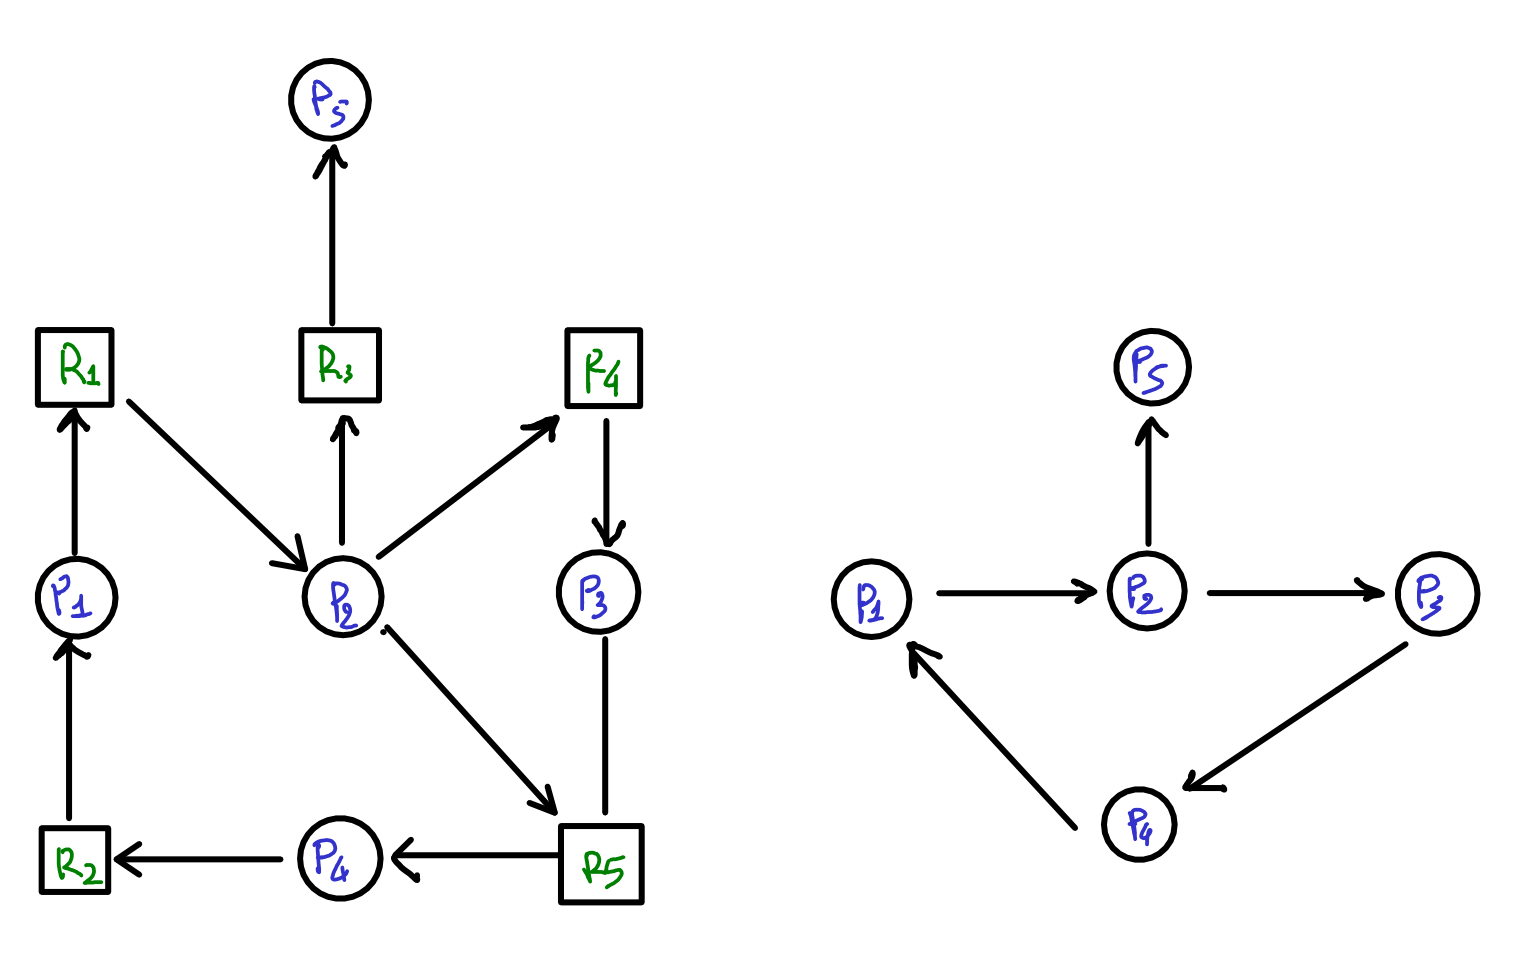
\includegraphics[scale=0.25]{RAG-detection}
\end{center}
Esempio di RAG a sinistra, e del \emph{grafo d'attesa} corrispondente a destra.
In figura un esempio di RAG a sinistra, e del \emph{grafo d'attesa} corrispondente a destra.

\subsection{Algoritmo di rilevazione}
Se nel sistema si hanno pi\`u istanze per tipo di risorsa non \`e possibile applicare il modello con RAG. In questi casi si utilizza un algoritmo simile a quello del banchiere. 

L'algoritmo di rilevazione si basa sull'esplorazione di ogni possibile sequenza di allocazione per i processi che non hanno ancora terminato. Se la sequenza va a buon fine, il sistema \`e ancora in uno stato safe, quindi non c'\`e deadlock. 

Per questo algoritmo necessitiamo di alcune strutture dati: 
\begin{lstlisting}[language=C]
int available[m];	 /* num. istanze di Ri disponibili */
int alloc[n][m];	 /* matrice di allocazione corrente */
int req_vec[n][m]; /* matrice delle richieste */
\end{lstlisting}

La sequenza safe in questo caso esiste se il sistema riesce a soddisfare le richieste attuali (sulla matrice delle richieste).

\subsubsection{Codice algoritmo}

\begin{lstlisting}[language=C]
int work[m] = available[m];
bool finish[] = (FALSE, /*...*/ , FALSE);
bool found = TRUE;
while (found) {
	found = FALSE;
	for (i = 0; i < n && !found; i++) {
		/* cerca un Pi con richiesta soddisfacibile */
		if (!finish[i] && req_vec[i][] <= work[]) {
			/* assume ottimisticamente che Pi esegua fino al 
			 * termine e che quindi restituisca le risorse;
			 * se cosi non fosse il possibile deadlock verra'
			 * evidenziato alla prossima esecuzione 
			 * dell'algoritmo. */
			 work[] = work[] + alloc[i][];
			 finish[i] = TRUE;
			 found = TRUE;
		}
	}
}
/* se finish[i] = FALSE per un qualsiasi i, 
 * Pi si trova in deadlock */
\end{lstlisting}
La complessit\`a di questo algoritmo \`e in $O(m*n^2)$.

\newpage
\subsection{Esempio di rilevazione}

\begin{multicols}{2}
[Dato un sistema con cinque processi, $P_0$, $P_1$, $P_2$, $P_3$, $P_4$ e tre tipi di risorsa suddivisi in 7 istanze della risorsa $A$, 2 istanze della risorsa $B$ e 6 istanze della risorsa $C$. Al tempo $T_0$ il sistema \`e nel seguente stato: ]


\begin{center}
\begin{tabular}{||c | c  c  c || }
 & \underline{Alloc.} & \underline{Req.} & \underline{Avail.}  \\
 & \emph{A B C} & \emph{A B C} & \emph{A B C} \\
 $P_0$ & 0 1 0 & \colorbox{green!40}{0 0 0} &  \colorbox{teal!40}{0 0 0} \\
 $P_1$ &2 0 0 & \colorbox{orange!40}{2 0 2} &  \\
 $P_2$ & 3 0 3 & \colorbox{blue!40}{0 0 0} &  \\
 $P_3$ & 2 1 1 & 1 0 0 & \\
 $P_4$ & 0 0 2 & 0 0 2 & \\
 \end{tabular}
 \end{center}

Se la colonna \emph{Available} \`e tutta a 0 e se tutte le righe della colonna \emph{Request} avessero almeno un valore diverso da 0 saremmo in deadlock. In questo caso abbiamo $P_0$ e $P_2$ che possono essere in \emph{ready queue} oppure in \emph{CPU}.
\end{multicols}

Verifichiamo se il sistema \`e in deadlock. Al tempo $T_0$ abbiamo che:
\begin{itemize}
\item \colorbox{teal!40}{$work = (0,0,0)$};
\item \colorbox{green!40}{i =0}; 
\begin{lstlisting}[language=C]
req_vec[0] = (0,0,0) <= work[]; 	/* OK */
work = work + (0,1,0);
\end{lstlisting}
\item \colorbox{orange!40}{i=1};
\begin{lstlisting}[language=C]
req_vec[1] = (2,0,2) <= work[]; /* NO */
\end{lstlisting}
\item \colorbox{blue!40}{i =2}; 
\begin{lstlisting}[language=C]
req_vec[0] = (0,0,0) <= work[]; 	/* OK */
work = work + (3,0,3);
\end{lstlisting}
\item Al termine dell'algoritmo si ottiene che la sequenza $\langle P_0, P_2, P_3, P_1, P_4 \rangle$ dar\`a \texttt{finish[i] = TRUE} per ogni $i$.
\end{itemize}


\begin{multicols}{2} 
[Supponiamo ora che il processo $P_2$ richieda un'altra istanza di tipo $C$. Lo stato viene modificato come segue:]
\begin{center}
\begin{tabular}{||c | c  c  c || }
 & \underline{Alloc.} & \underline{Req.} & \underline{Avail.}  \\
 & \emph{A B C} & \emph{A B C} & \emph{A B C} \\
 $P_0$ & 0 1 0 & 0 0 0 &  0 0 0 \\
 $P_1$ &2 0 0 & 2 0 2 &  \\
 $P_2$ & 3 0 3 & \colorbox{red!40}{0 0 1} &  \\
 $P_3$ & 2 1 1 & 1 0 0 & \\
 $P_4$ & 0 0 2 & 0 0 2 & \\
 \end{tabular}
 \end{center}
Ora il sistema \`e in stallo. Anche liberando le risorse di $P_0$, \emph{Available} non ha sufficienti risorse per soddisfare le richieste degli altri processi. Il sistema va in deadlock: $\langle P_1, P_2, P_3, P_4 \rangle$.
\end{multicols}

\subsection{Ripristino}

L'algoritmo di rilevazione pu\`o essere chiamato secondo diversi paradigmi:
\begin{itemize}
\item Dopo ogni richiesta non soddisfatta e se la \emph{ready queue} \`e vuota. Questo metodo necessit\`a anche di verificare se la ready queue \`e vuota, aggiungendo tempo ``sprecato''.
\item Ogni $N$ secondi, ci si accorge per\`o che il deadlock non \`e molto frequente, e questo metodo porterebbe ad uno spreco di risorse e tempi di CPU.
\item Quando l'utilizzo della CPU scende sotto una soglia $T$.
\end{itemize}

Una volta rilevato uno stallo, questo si pu\`o affrontare in due modi. Il primo prevede la \emph{terminazione} di uno o pi\`u processi, per interrompere l'\emph{attesa circolare}; il secondo consiste nell'esercitare la prelazione su alcune risorse in possesso di uno o pi\`u processi in stallo.

\subsubsection{Terminazione dei processi}
Per eliminare le situazioni di stallo attraverso la terminazione di processi si possono adoperare due metodi:
\begin{itemize}
\item \textbf{Terminazione di tutti i processi in stallo}. Operazione molto onerosa ma che interrompe \emph{sicuramente} il deadlock.
\item \textbf{Terminazione di un processo alla volta}. Procedendo fino all'eliminazione del ciclo di stallo e, di conseguenza, dopo aver terminato ogni processo si deve invocare un algoritmo di rilevamento per stabilire se esistono ancora processi in stallo, aumentando l'overhead.
\end{itemize}


\subsubsection{Prelazione di risorse}

Per eliminare un deadlock utilizzando la \emph{prelazione sulle risorse} si devono considerare alcuni fattori:

\begin{enumerate}
\item \textbf{Selezione di una vittima}. Occorre stabilire quali risorse e quali processi si devono sottoporre a prelazione. \`E necessario stabilire l'ordine di prelazione allo scopo di minimizzare i costi. I fattori di costo possono includere parametri come il numero di risorse possedute da un processo in deadlock e la quantit\`a di tempo gi\`a spesa durante l'esecuzione del processo. 
\item \textbf{Rollback}. Poicc\'e un processo sottoposto a prelazione non pu\`o proseguire normalmente, \`e necessario ricondurlo ad un precedente stato \emph{safe} dal quale pu\`o poi essere riavviato. 
\item \textbf{Total rollback}. In generale \`e difficile determinare quale sia uno stato sicuro, la soluzione pi\`u semplice \`e di terminare il processo prelazionato e riavviarlo da zero.
\item \textbf{Rischio di starvation}. Se vengono prelazionato sempre lo stesso processo, il rischio che questo non possa terminare e vada in starvation aumenta. La soluzione a questo problema \`e di considerare il numero di \emph{rollback} nei fattori di costo del punto 1.
\end{enumerate}


\section{Conclusione}

\begin{itemize}
\item Un deadlock si verifica quando, in un insieme di processi, ciascun processo attende un evento che pu\`o essere causato solo da un altro processo dell'insieme.
\item Vi sono quattro condizioni necessarie per lo stallo: ($1$) mutua esclusione, ($2$) possesso e attesa, ($3$) assenza di prelazione e ($4$) attesa circolare. Una situazione di stallo \`e possibile solo quando sono verificate tutte e quattro le condizioni.
\item Gli stalli possono essere modellati mediante grafi di allocazione delle risorse (RAG) in cui un ciclo indica uno stallo.
\item \`E possibile prevenire gli stalli garantendo che non si verifichi una delle quattro condizioni necessarie per lo stallo. Tra le quattro possibilit\`a, eliminare l'attesa circolare \`e l'unico approccio pratico.
\item Lo stallo pu\`o essere evitato usando l'algoritmo del banchiere, che non concede risorse se cos\`i facendo si indurrebbe il sistema in uno stato \emph{unsafe} in cui si potrebbe verificare un deadlock.
\item Un algoritmo di rilevamento degli stalli pu\`o esaminare i processi e le risorse su un sistema di esecuzioe per determinare se un insieme di processi si trova in una situazione di stallo.
\item Un sistema pu\`o tentare di recuperare da una situazione di stallo interrompendo uno dei processi nell'attesa circolar o esercitando la prelazione sulle risosre che sono state assegnate ad un processo in deadlock.
\end{itemize}


% Lezione del 20/03/2023. 
% Testo di riferimento Silberschatz-Galvin capitolo 9, pagina 376
\chapter{Gestione della Memoria}

\section{Introduzione}

La CPU, attraverso il program counter, va ad indicizzare locazioni di memoria all'interno delle quali \`e presente la prossima istruzione da eseguire. Si hanno quindi le fasi di \emph{fetch}, nella quale viene l'istruzione inserita instruction register della CPU, poi avviene la fase di  \emph{decode}, ovvero la verifica dell'opcode dell'istruzione per determinare cosa fare, avviene l'eventuale recupero degli operandi dalla \emph{memoria}, fase di \emph{execute} ed infine la fase di \emph{write back}, nella quale si va a salvare nella memoria eventuali risultati.
Come si pu\`o notare la memoria \`e coinvolta in ogni fase dell'esecuzione di un processo.
Ogni processo necessita dunque di un'area di memoria riservata, chiamata \emph{spazio di indirizzamento}. 

Uno dei compiti del sistema operativo sara\`a quindi quello di dividere la memoria, che \`e una risorsa condivisa, tra tutti i processi che ne fanno richiesta. Una volta che questa zona di memoria \`e stata allocata per un processo, entra in gioco anche un sistema di protezione: solo il processo a cui \`e stata concessa la memoria pu\`o accedere, a meno che non venga condivisa con altri, ma in quel caso dev'essere messo in atto un meccanismo di mutua esclusione.

Inoltre, esiste il concetto di \emph{memoria virtuale} che aggiunge l'area di \emph{swap} e la possibilit\`a di far credere ad un processo che il suo spazio di indirizzamento sia pi\`u ampio di quello realmente concesso.

\subsection{Vincolo}
Ogni programma deve essere portato in memoria e trasformato in un processo per essere eseguito.
Si deve dunque trasformare un programma sorgente, con \emph{indirizzi simbolici} in un processo caricato in memoria, con \emph{indirizzi fisici}. 

\subsection{Come avviene la trasformazione?}

Si crea un mapping tra lo spazio logico del processo e lo spazio fisico in memoria. Prendendo un programma sorgente compilato e dire dove ogni sua parte \`e situata nella memoria fisica. Il \emph{compilatore} associa gli indirizzi simbolici ad indirizzi rilocabili. Successivamente il \emph{linker e il loader}, associano gli indirizzi rilocabili a indirizzi assoluti, ovvero il vero indirizzo in cui il dato o l'istruzione si trover\`a in memoria.

\subsubsection{Fasi della Trasformazione}
\begin{center}
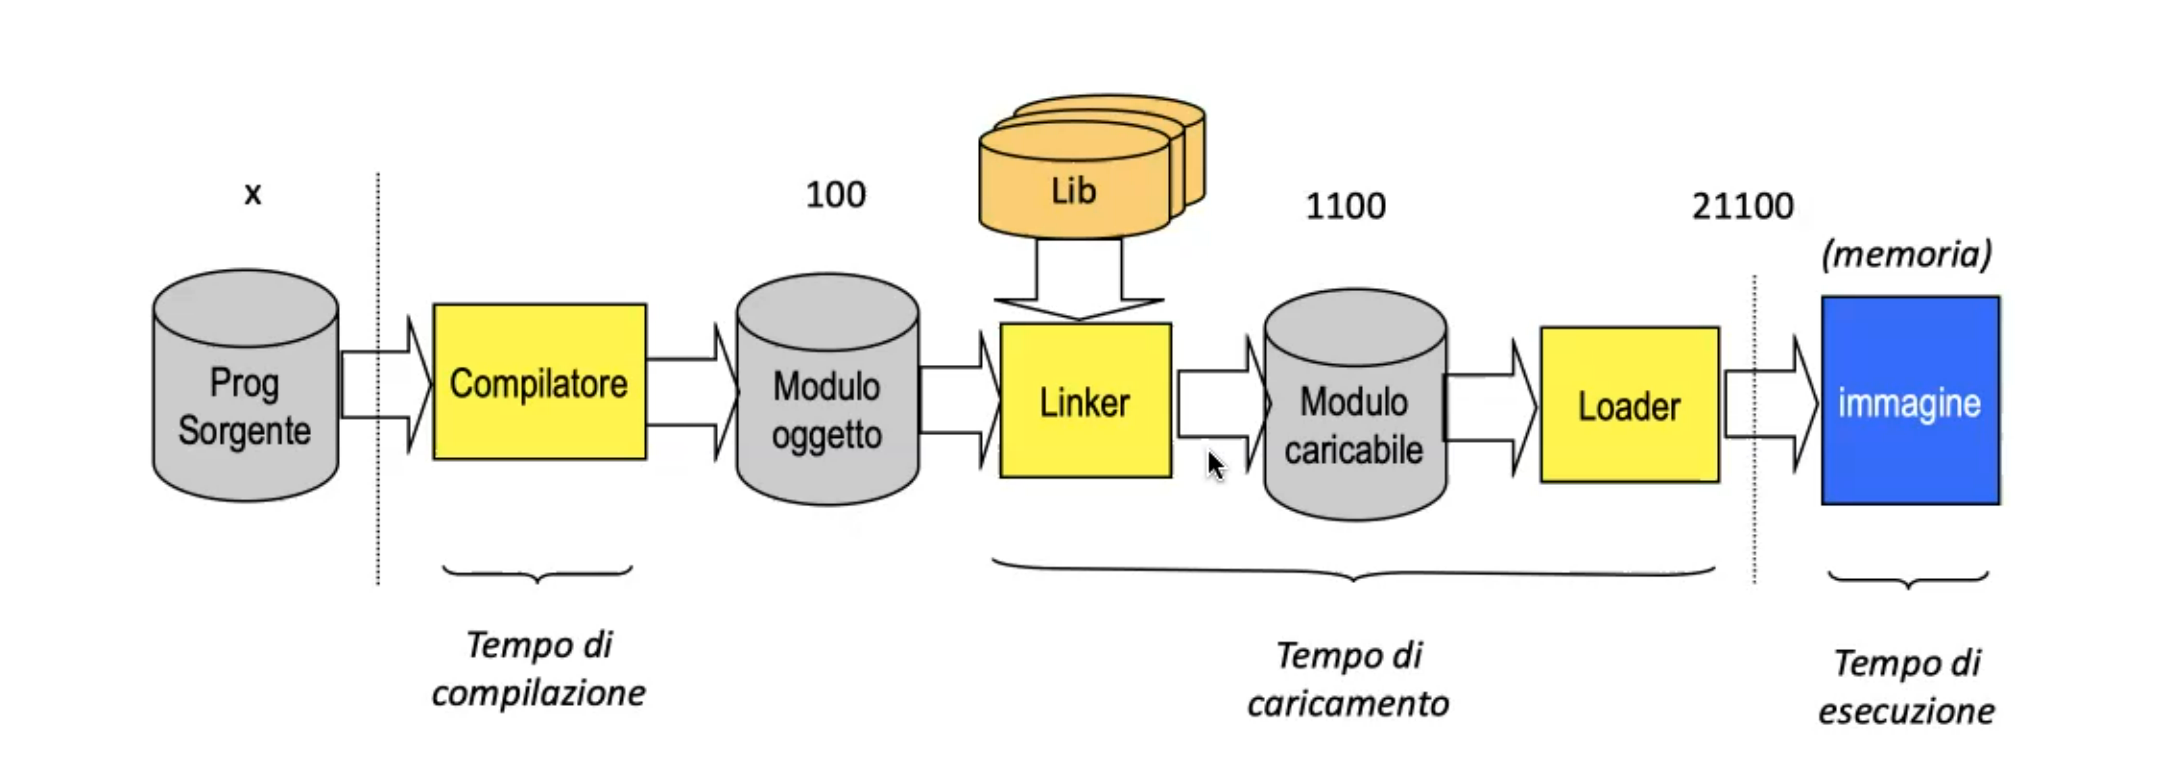
\includegraphics[scale=0.2]{trasf}
\tiny{\textbf{Modulo caricabile}: file eseguibile}
\end{center}
\begin{itemize}
\item Gli indirizzi hanno diverse rappresentazioni nelle varie fasi di costruzione di un programma.
\item Il collegamento tra indirizzi simbolici e fisici viene detto \textbf{binding}.
\end{itemize}

\section{Binding dati/istruzioni e indirizzi di memoria}

Il concetto di binding degli indirizzi \`e determinato da come il sistema operativo agisce, da non confondere con la differenza tra linguaggi compilati o interpretati.

\subsection{Compile time}

Il binding avviene al tempo di compilazione, in questo caso saranno assenti linker e loader. 
Il programma ottenuto avr\`a  un eseguibile che verr\`a caricato in memoria sempre nella 
stessa locazione, se si vuole cambiare la posizione di qualche simbolo si deve ricompilare 
tutto il programma.  Nononostante questa soluzione presenti degli svantaggi, ovvero il 
contesto non \`e flessibile, pu\`o essere utile per task dedicati o per ottimizzare al 
massimo: non si ha overhead per la gestione della memoria.

\subsection{Load time}

Il binding avviene al tempo di caricamento, sono quindi necessari linker e loader. \`E necessario generare codice rilocabile, attraverso indirizzi relativi (ad esempio 128 byte dall'inizio del programma). In questo caso, se cambia l'indirizzo di riferimento, devo ricaricare.

\subsection{Run time}

Il binding \`e posticipato se il processo pu\`o essere spostato durante l'esecuzione in 
posizioni diverse della memoria. Supponiamo che un processo venga sospeso e il suo stato sia
salvato nell'area di \emph{swap}; quando viene ripristinato, se il binding fosse avvenuto a
tempo di compilazione, dovrebbe essere ricaricato nell'area di memoria in cui era 
precedentemente. Questo non \`e sempre possibile, perch\'e la memoria potrebbe essere in uso 
da altri processi. Il binding a tempo di esecuzione permette perci\`o di rilocare il processo
in un'area di memoria differente da quella precedente alla sospensione e ripristinare 
l'esecuzione da dove era stata interrotta. 

\paragraph{Swap} $\to$ Tutto il processo \`e attivo o non attivo. 
\paragraph{Memria virtuale} $\to$ Alcune parti del processo sono in memoria (RAM) mentre le altre sono su disco.


\subsection{Binding Statico e Binding Dinamico}

Si dice \emph{Binding Statico} quando gli indirizzi restano invariati per tutta la vita del processo dopo che \` stato caricato, ovvero quando si utilizza il binding a compile time oppure quello a load time.

Si dice \emph{Binding Dinamico} quando viene utilizzato il binding a tempo di esecuzione. In questo caso un eventuale ricaricamento pu\`o avvenire in altre posizioni di memoria. 

Il rischio dell'utilizzo di un binding dinamico \`e che un processo che "esce" dalla memoria, potrebbe non trovare spazio in futuro.

\subsubsection{Esempio di binding}
\begin{center}
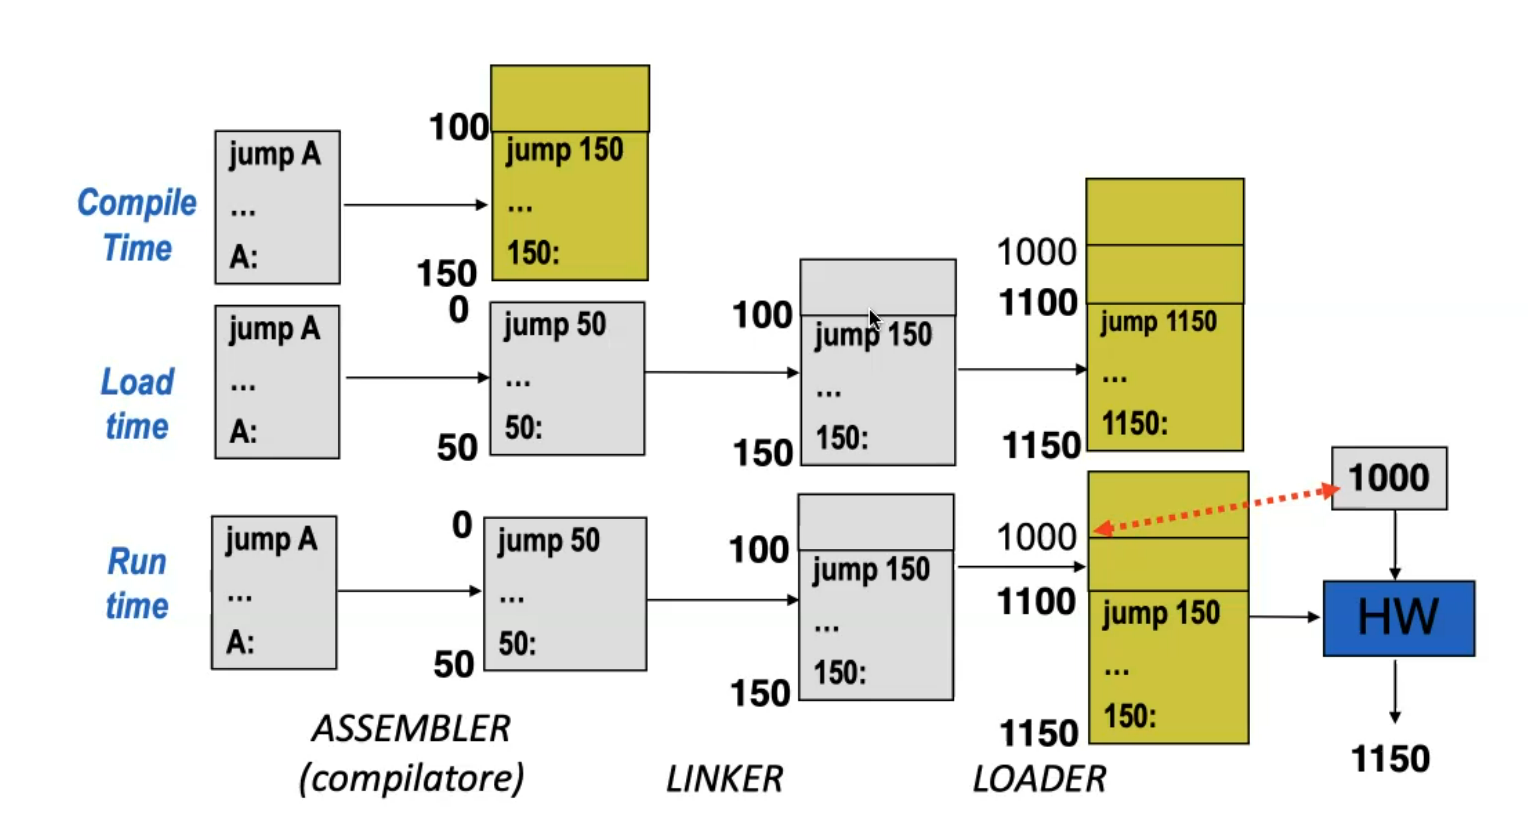
\includegraphics[scale=0.2]{bindingExample}
\end{center}

\subsection{Linking statico o dinamico}

Anche il linker si divide in statico o dinamico.

\begin{itemize}
    \item Linking statico: \`e il linking tradizionale in cui tutti i riferimenti sono
        definiti prima dell'esecuzione. L'immagine del processo contiene una copia delle
        librerie usate. Si avr\`a un eseguibile grande e pi\`u lento all'avvio, ma pi\`u 
        veloce in esecuzione. 
    \item Linking dinamico: in questo caso il linking delle librerie \`e posticipato al 
        tempo di esecuzione. Il codice non contiene una copia delle librerire usate ma 
        solo dei riferimenti (stub) per poterle recuperare. Questo eseguibile sar\`a 
        pi\`u rapido all'avvio e occuper\`a meno memoria, ma sar\`a pi\`u lento in 
        fase di esecuzione, perch\'e dovr\`a recuperare le librerie ogni volta che
        saranno necessarie.
\end{itemize}

\subsection{Loader statico e dinamico}

\begin{itemize}
    \item Loading statico: tradizionale, ovvero quando tutto il codice \`e caricato in 
        memoria al tempo di esecuzione. Il vantaggio \`e una maggior velocit\`a in 
        esecuzione a discapito di un maggior costo per il caricamento ed una memoria 
        occupata maggiore.
    \item Loading dinamico: caricamento posticipato dei moduli in corrispondenza del primo 
        utilizzo. Il codice non utilizzato non viene caricato, utile per codice con molti 
        casi speciali. Il vantaggio di questo metodo \`e un avvio molto rapido ed il minor 
        spazio occupato in memoria; di contro l'esecuzione sar\`a pi\`u lenta se dovesse 
        servire tutto ci\`o che non \`e stato caricato.
\end{itemize}

\section{Spazi di indirizzamento}

Lo spazio di \emph{indirizzamento logico} dev'essere legato allo spazio di 
\emph{indirizzamento fisico}.
\begin{itemize}
\item L'indirizzo \emph{logico} (o \emph{virtuale}) \`e sempre contiguo.  \`E generato dalla CPU. 
\item L'indirizzo \emph{fisico} \`e lo spazio di indirizzamento \underline{visto dalla memoria}, non necessariamente \`e contiguo.
\end{itemize}

Se il binding \`e a \emph{compile-time} o a \emph{load-time}, l'indirizzo logico e quello 
fisico \emph{coincidono}. In questo caso la vista della CPU \`e uguale alla vista della 
memoria.

Se il binding \`e a \emph{run-time} l'indirizzo fisico e logico sono generalmente diversi.
In questo caso la vista della CPU sar\`a sempre continua ma diversa dalla vista della memoria.

\section{Binding: Statico vs Dinamico}

\begin{center}
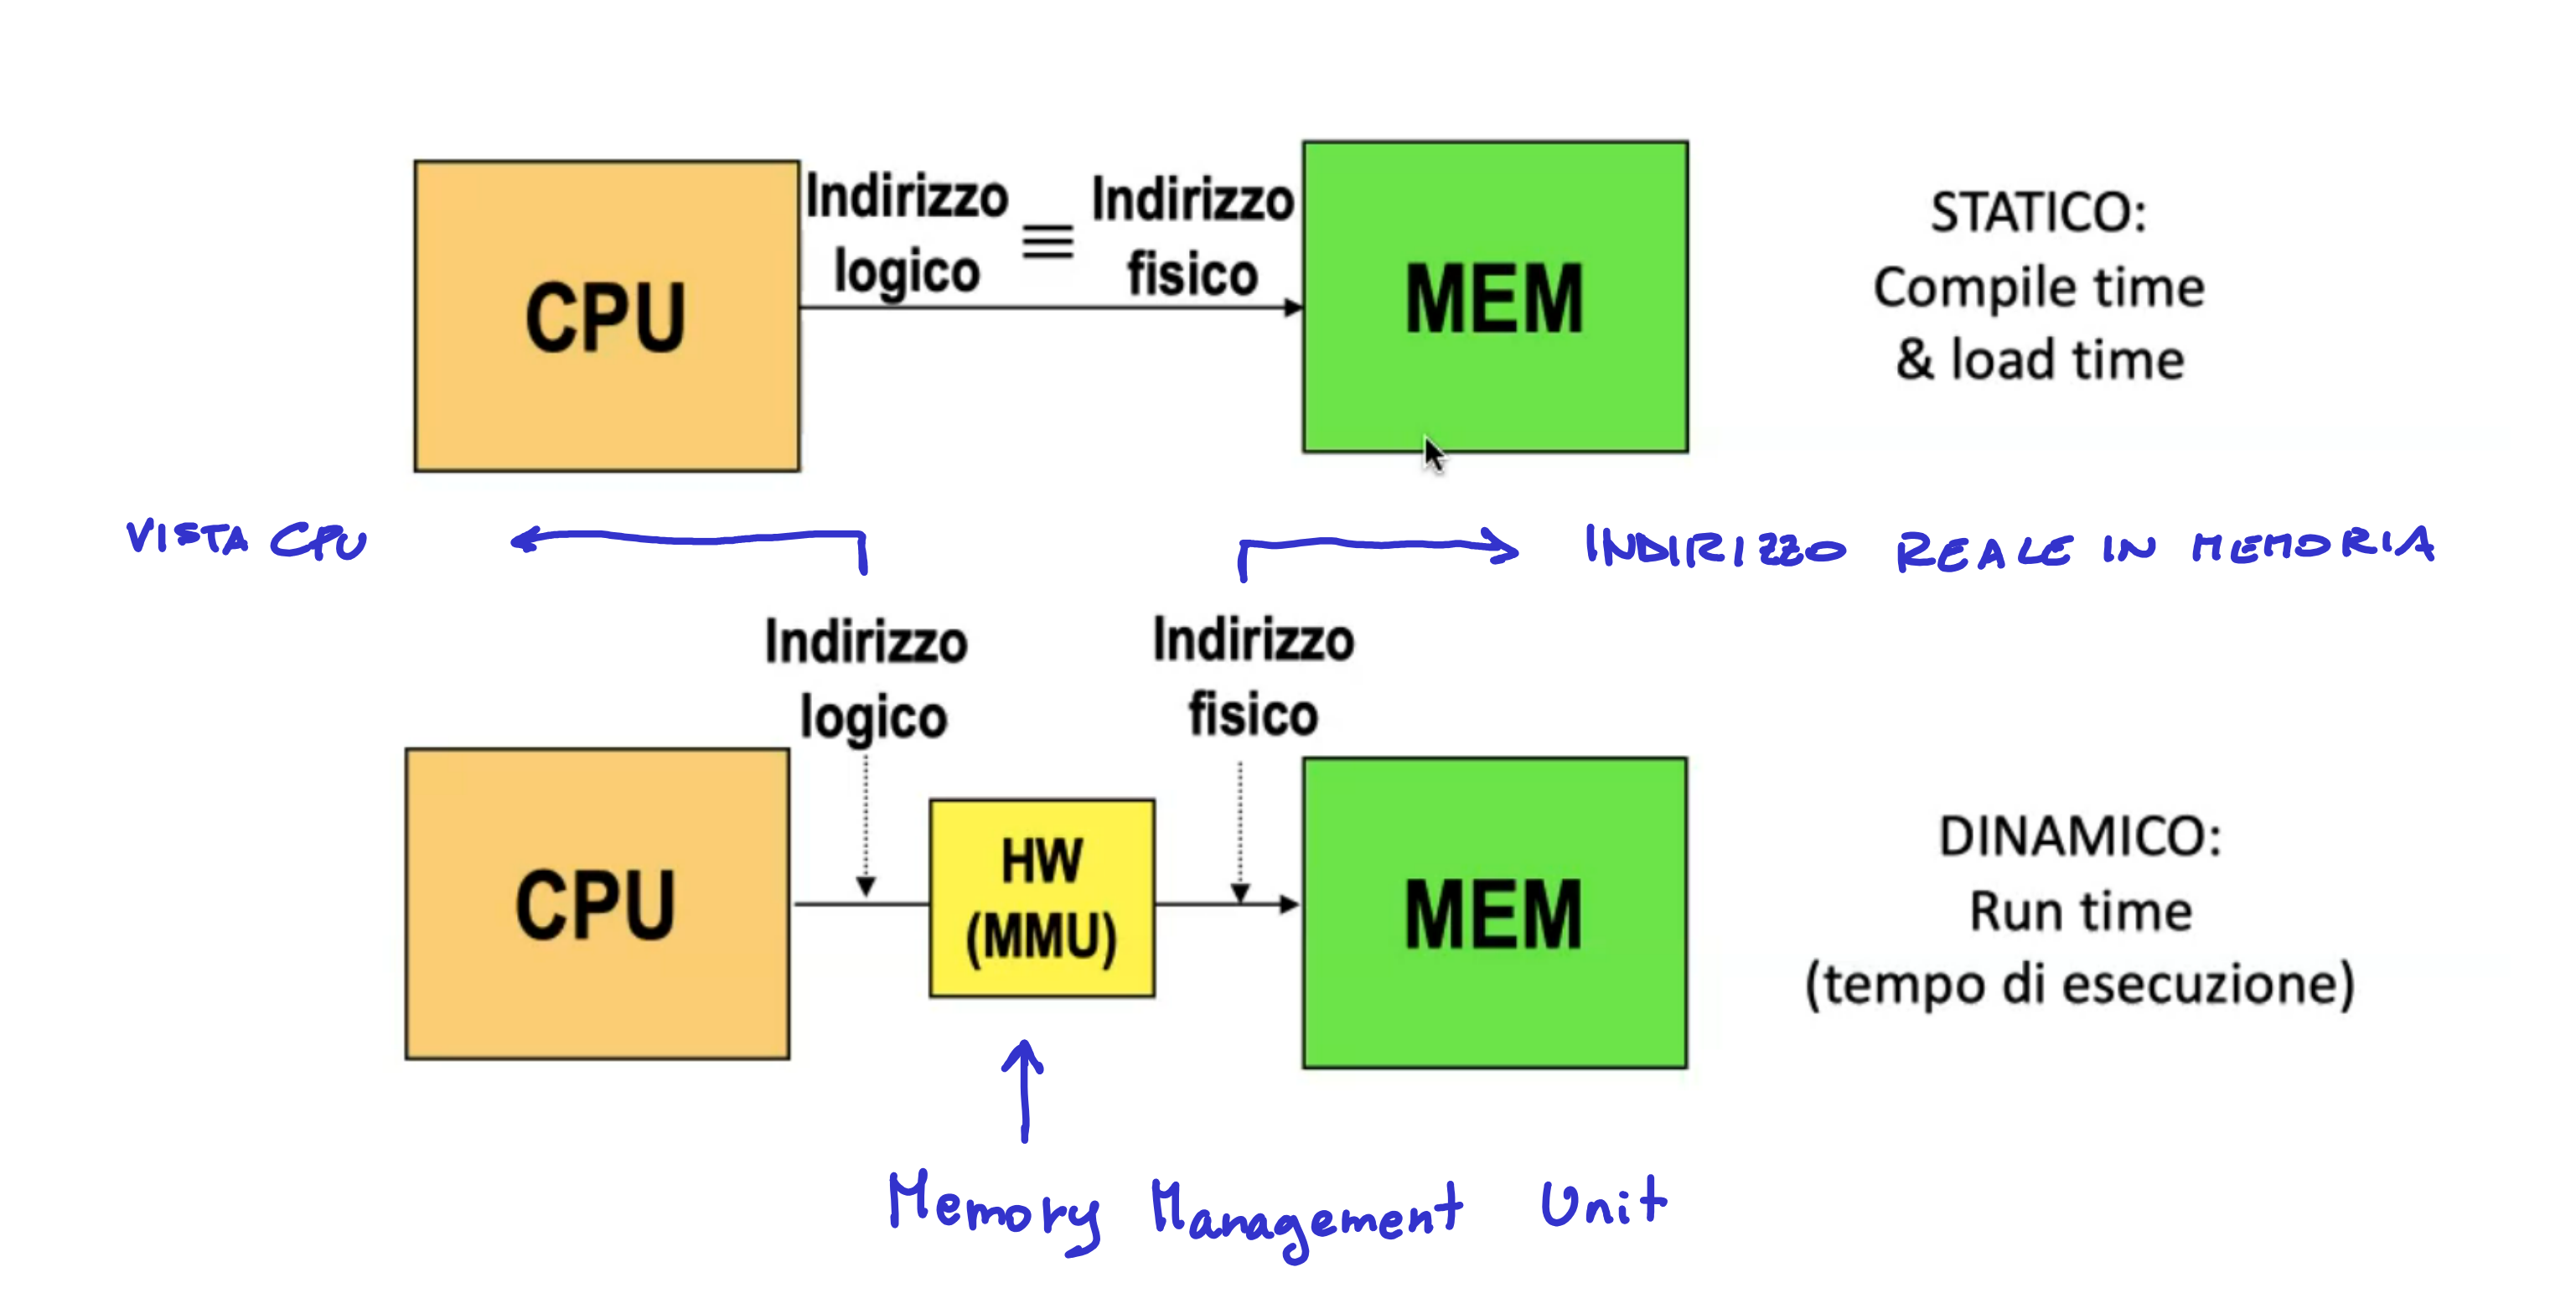
\includegraphics[scale=0.15]{staticVsDynamic}
    \tiny{\textbf{MMU}: Hardware che mappa l'indirizzo logico in quello fisico reale.} 
\end{center}

\subsection{Memory Management Unit - MMU}

\`E un dispositivo hardware che mappa indirizzi virtuali (logici) in indiriizzi fisici.

\subsubsection{Schema base dell'MMU}
Il valore del registro di rilocazione \`e aggiunto a ogni indirizzo generato da un processo 
e inviato alla memoria. 

\begin{center}
    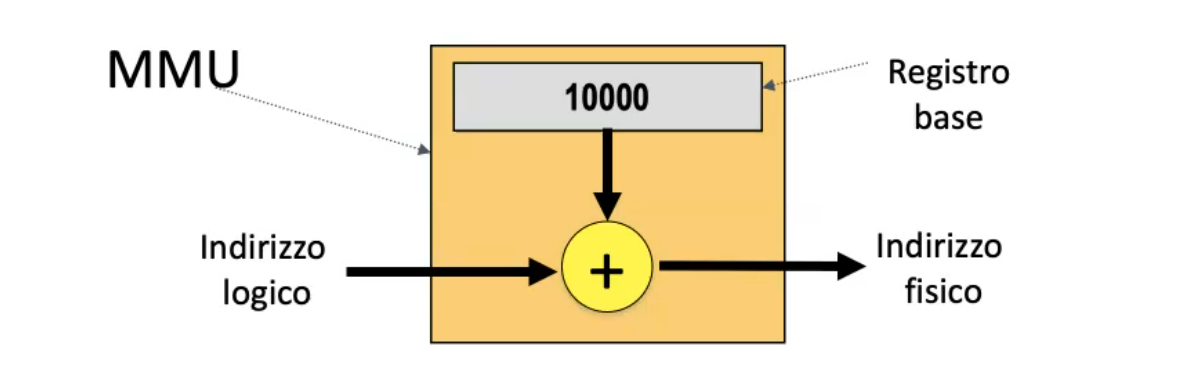
\includegraphics[scale=0.3]{mmu}
\end{center} 
\paragraph{Registro base} $\to$ indica il punto d'inizio del blocco contiguo dello spazio di 
        indirizzo del processo.

L'MMU viene aggiornata ad ogni \emph{context-swicth}.

\subsection{Considerazioni}

\begin{enumerate}
    \item In un sistema multiprogrammato non noto in anticipo dove un processo si trova in 
        memoria, quindi si esclude il binding a tempo di compilazione. 
    \item L'esigenza di avere uno \emph{swap} impedisce l'utilizzo di indirizzi rilocati in 
        modo statico, quindi il binding a tempo di caricamento non \`e possibile. 
\end{enumerate}

Di conseguenza, nei sistemi general purpose, si utilizza una \emph{rilocazione dinamica}, 
mentre la \emph{rilocazione statica} diventa utile in sistemi per applicazioni specifiche in 
cui le risorse sono limitate o \`e necessaria molta ottimizzazione.


\section{Allocazione contigua}

I processi sono allocati in memoria in posizioni contigue all'interno di una partizione. La 
memoria \`e suddivisa in \emph{partizioni fisse} e \emph{partizioni variabili}. Per esempio 
un processo con dimensione dell'immagine di 10kB, occuper\`a 10kB consecutivi. 

\subsection{Tecnica delle partizioni fisse}

La memoria \`e un insieme di partizioni di dimensioni predefinite, tipicamente di dimensioni 
diverse. Il Sistema Operativo deve assegnare ai job degli spazi abbastanza grandi per 
contenerli. Se lo spazio non \`e sufficiente i job dovranno attendere. 

\subsubsection{Vincoli:}
\begin{enumerate}
    \item Posso avere al massimo $n$ processi in esecuzione contemporaneamente, dove $n$ \`e 
        il numero di partizioni.
    \item Se arriva un processo pi\`u grande di ogni partizione, non potr\`a mai 
        andare in esecuzione. 
    \item All'arrivo di un processo ci sono due spazi disponibili sufficientemente capienti
        per farcelo stare, in quale delle partizioni lo inserisco?
\end{enumerate}

\subsubsection{Assegnazione della memoria}
\begin{multicols}{2}[
L'assegnazione della memoria \`e effettuata dallo scheduling a lungo termine, esistono due 
opzioni: ]

    \begin{itemize}
        \item Una coda per ogni partizione
    \end{itemize}
    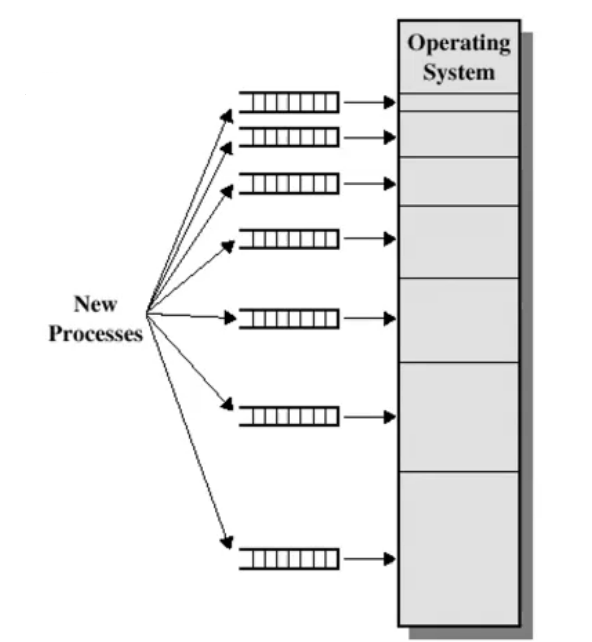
\includegraphics[scale=0.2]{multiQueue}
    \begin{itemize} 
        \item Coda singola 
    \end{itemize}

    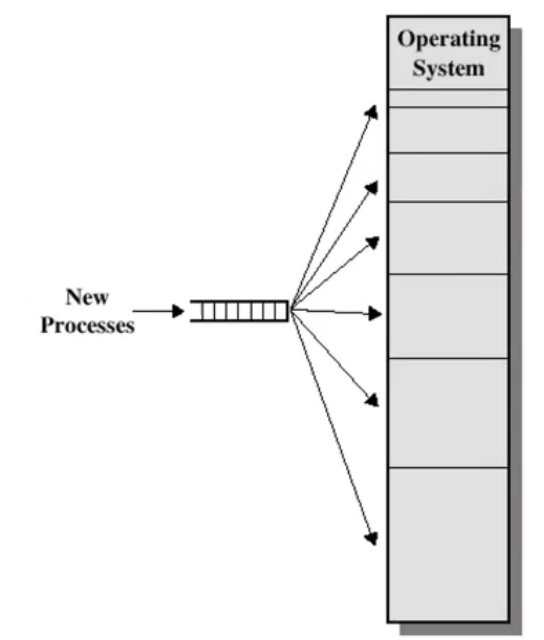
\includegraphics[scale=0.2]{singleQueue}
\end{multicols}

\subsubsection{Una coda per partizione}
Il processo viene assegnato alla partizione pi\`u piccola in grado di contenerlo. Questo
schema \`e poco flessibile: possono esserci partizioni vuote e job nelle altre code.

\subsubsection{Coda unica}
Unica coda con diverse politiche di gestione:
\begin{itemize}
    \item FCFS: una coda di tpo FIFO, molto semplice ma l'utilizzo della memoria potrebbe 
        essere scarso: il primo processo in coda \`e molto grande e fa attendere altri 
        processi pi\`u piccoli. 
    \item Best-fit-only: il sistema operativo scansiona tutta la coda ogni volta che una 
        partizione si libera e scelglie il job con le dimensioni pi\`u simili alla partizione.
        In questo caso si incorre nel rischio di starvation.
    \item Best-available-fit: simile a quella precedente ma sceglie il primo job che pu\`o 
        stare nella partizione. Anche in questo caso si incorre nel rischio di starvation. 
\end{itemize}

\emph{Best-fit-only} e \emph{Best-available-fit} sono tecniche di "scavalco", in entrambi i
casi, oltre al rischio di starvation, aumentano i costi di gestione, e conseguentemente si 
riducono i tempi di esecuzione della CPU. 

\subsubsection{Supporto per la rilocazione dinamica}

L'MMU consiste di \emph{registri di rilocazione} per proteggere lo spazio dei vari processi 
(attivamente e passivamente). I registri contengono:
\begin{itemize}
    \item Valore dell'indirizzo pi\`u basso (registro base o di rilocazione).
    \item Limite superiore dello spazio logico (registro limite).
\end{itemize}
Ogni indirizzo logico deve risultare minore del limite. 

\subsubsection{Supporto per la rilocazione}

\begin{center}
    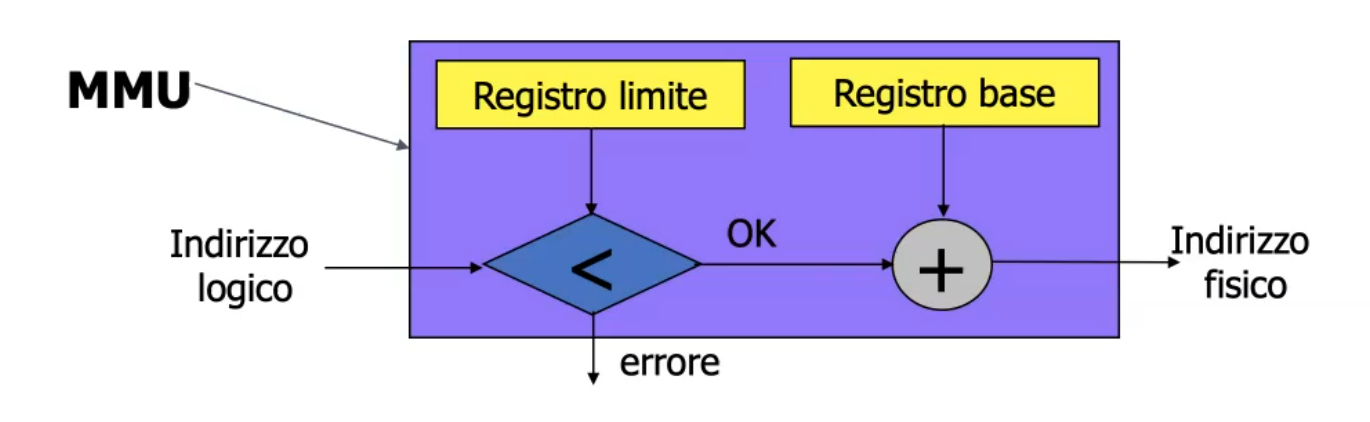
\includegraphics[scale=0.25]{mmuRelocation}
    \begin{itemize}

        \item L'errore incorre quando si cerca di accedere ad una partizione non detenuta dal processo.
        \item Indirizzo superiore alla grandezza del processo genera segmentation fault.
        \end{itemize}
    
\end{center}

\subsubsection{Considerazioni}

Il vantaggio della tecnica con partizioni fisse \`e la relativa semplicit\`a. Abbiamo anche 
numerosi svantaggi:
Il grado di multiprogrammazione \`e limitato dal numero di partizioni. Si ha dello spreco di 
memoria, detto \emph{frammentazione}, che si divide in frammentazione interna ed esterna.
\begin{itemize}
    \item \textbf{Frammentazione interna:} \`e si ha quando la dimensione della partizione \`e pi\`u grande della dimensione del job. 
    \item \textbf{Frammentazione esterna:} quando vi sono partizioni non utilizziate che 
        soddisfano le esigenze dei processi in attesa.
\end{itemize}

\subsection{Tecnica delle partizioni variabili}

Questa tecnica elimina la frammentazione \emph{interna}, ma con il rischio di aggravare la 
frammentazione \emph{esterna}.

Con questo schema lo spazio utente \`e diviso in partizioni di dimensioni variabili, identiche
alla dimensione dei processi. 

\subsubsection{Assegnazione della memoria}

La memoria \`e vista come un unico grande spazio contiguo, all'arrivo di un processo il 
sistema operativo assegna uno spazio di memoria della dimensione del processo. Cosi via 
ogni volta che un nuovo processo viene avviato. Al termine dei processi, questi ultimi 
liberano la memoria a loro assegnata, creando una serie di \emph{buchi} (\emph{hole}) che, 
se sono vicini possono essere fusi in un buco pi\`u grande, se sono distanti non possono 
essere accorpati. Questi buchi possono essere riallocati al bisogno, ma la memoria evolve
in una situazione come quella nell'immagine sottostante. 
\begin{center}
    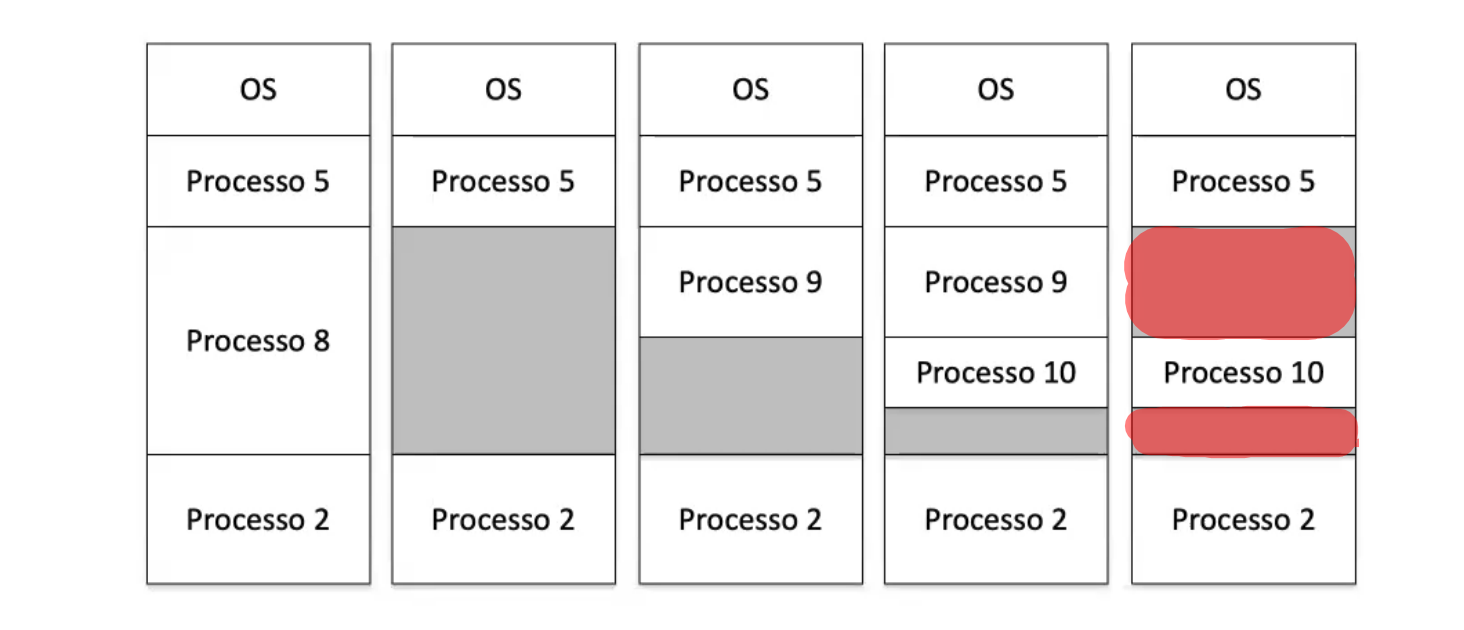
\includegraphics[scale=0.2]{varHoleEx}
\end{center} 
La frammentazione esterna non \`e stata eliminata. Se ad esempio ci fosse un processo in 
attesa che occupa quanto lo spazio evidenziato in rosso, dovrebbe restare in attesa.

\paragraph{First-fit} $\to$ Primo slot di memoria disponibile che pu\`o contenere il processo.
Richiede una \underline{ricerca parziale}, ad esclusione del caso pessimo in cui lo spazio 
libero \`e l'ultimo della lista.
\paragraph{Worst-fit} $\to$ \underline{Ricerca completa} del \emph{buco} pi\`u grande 
disponibile, cos\`i posso allocare altro nella zona rimanente. 
\paragraph{Best-fit} $\to$ \underline{Ricerca completa} del \emph{buco} pi\`u piccolo
disponibile che pu\`o contenere il processo. In questo modo si salvaguardano gli spazi 
maggiori per altri processi pi\`u grandi. 

\emph{First-fit} \`e tipicamente preferita per la velocit\`a. 

\subsubsection{Supporto per la rilocazione}

Come nel caso delle partizioni fisse, l'MMU possiede dei registri di rilocazione per 
proteggere lo spazio dei vari processi (attivamente e passivamente).

\begin{center}
    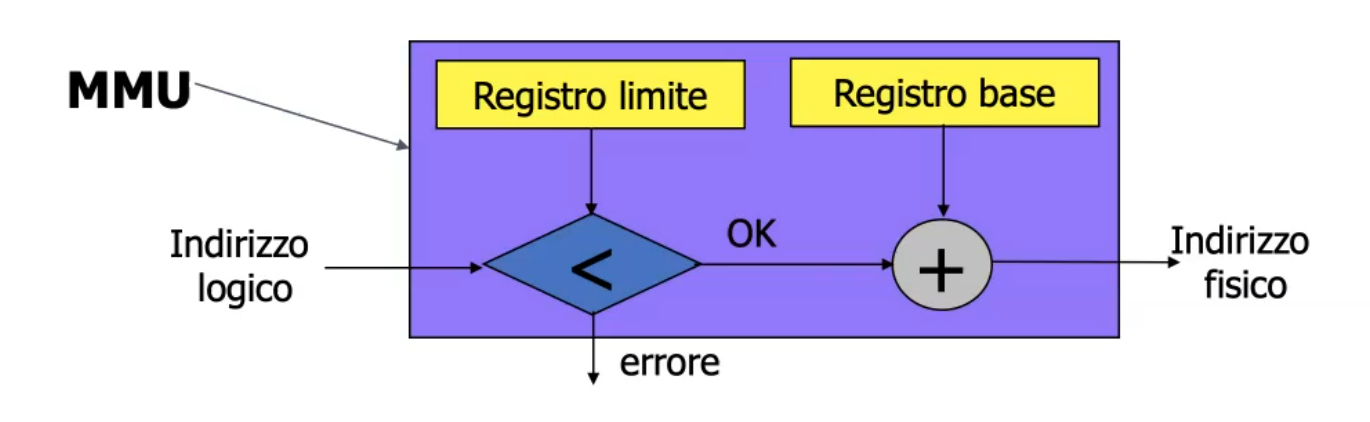
\includegraphics[scale=0.25]{mmuRelocation}
\end{center} 

\subsubsection{Considerazioni} 
Il vantaggio della tecnica delle partizioni variabili \`e che rimuove la frammentazione 
interna per costruzione. Gli svantaggi sono molteplici: rimane la frammentazione esterna. 
\begin{itemize}
    \item Esiste spazio disponibile in memoria, ma non \`e contiguo. 
    \item Con \emph{first-fit}, dati $N$ blocchi allocati, $0.5*N$ blocchi vanno persi. 
\end{itemize}

% Lezione del 30/03/2023 

\subsection{Tecnica della compattazione}
Questa tecnica prevede lo spostamento del contenuto della memoria in modo da rendere contigui i blocchi di un 
processo. \`E possibile solo se la rilocazione \`e dinamica e prevede la modifica del registro base. Tuttavia, questo 
metodo \`e costoso: \emph{quanta memoria sposto?}

\subsubsection{Compattazione della memoria}
\begin{multicols}{2}
\begin{center}
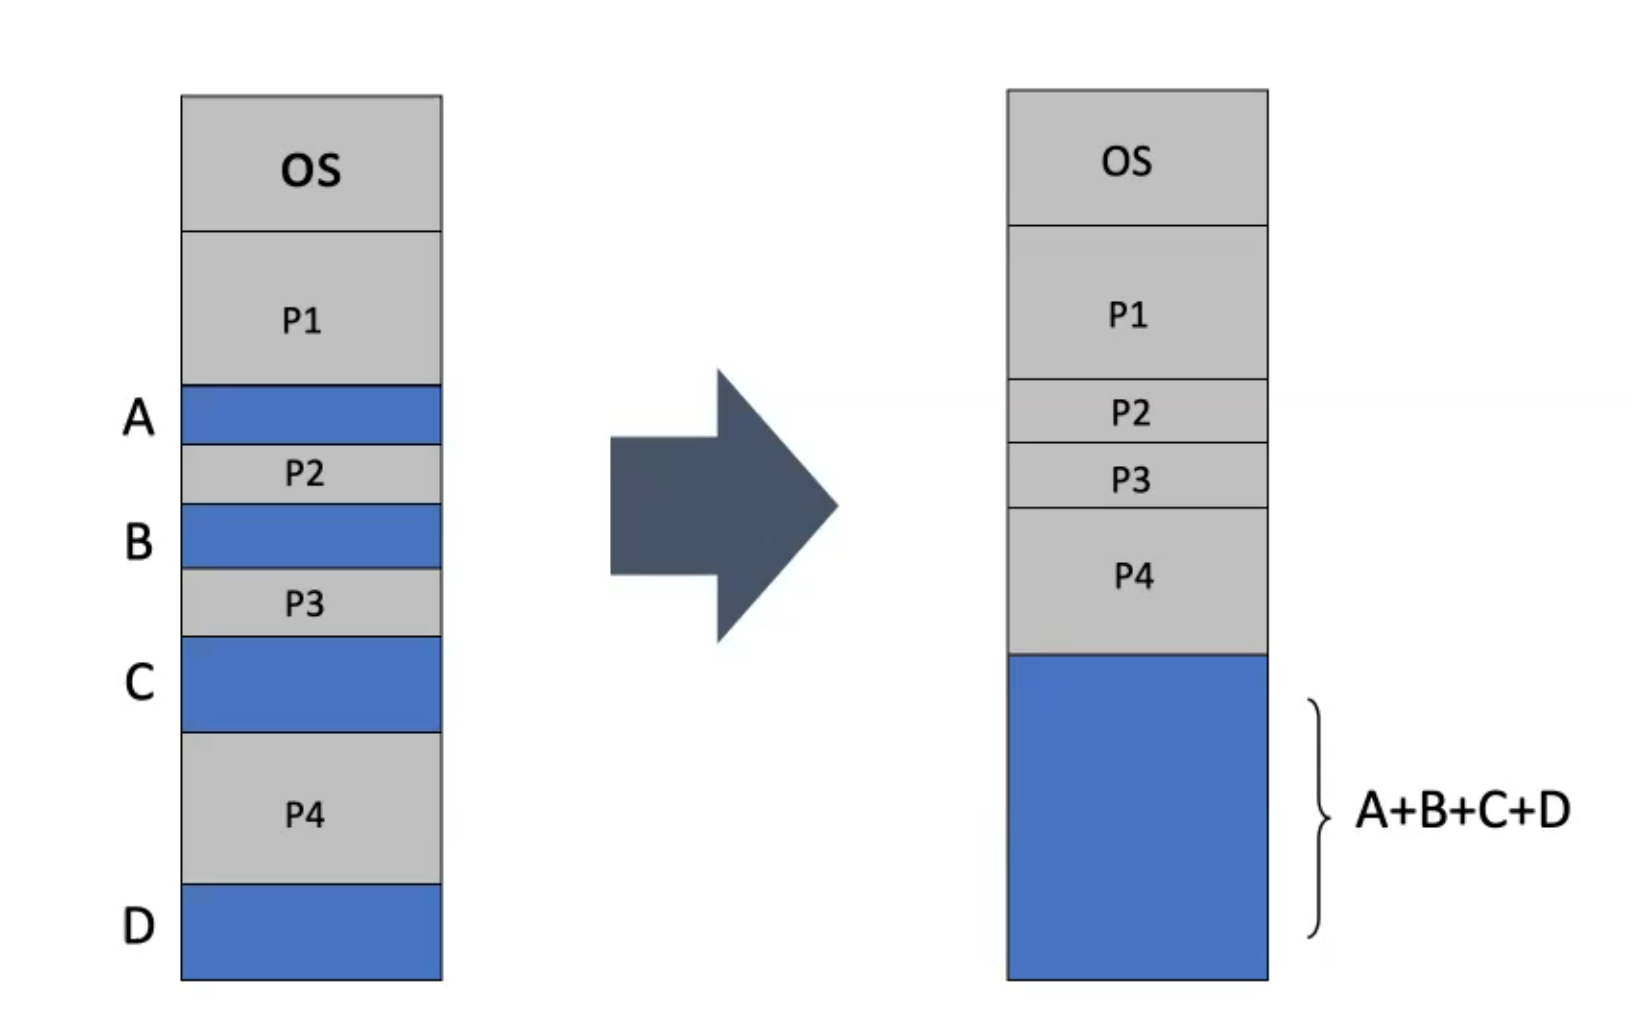
\includegraphics[scale=0.12]{comp_mem}
\end{center}

Non \`e sufficiente modificare il registro base, bisogna anche effettuare il \emph{trasferimento} della memoria allocata
alla nuova zona di allocazione. Questo significa che sono richieste operazioni di spostamento dati, che occupano il bus
della memoria, il DMA e, durante gli spostamenti, i processi coinvolti non possono lavorare. 
\end{multicols}
\subsection{Tecnica del buddy system}

Questa tecnica \`e un compromesso tra partizioni fisse e variabili. Anche in questo caso l'allocazione dei processi \`e 
contigua. La memoria \`e suddivisa in blocchi di dimensioni $2^k$, con $L<k<U$ e:
\begin{itemize}
\item $2^L$: \`e il pi\`u \emph{piccolo} blocco allocato. (Esempio: 4k)
\item $2^U$: \`e il pi\`u \emph{grande} blocco allocato. (Esempio: tutta la memoria).
\end{itemize}
Inizialmente la memoria \`e tutta disponibile: la lista di blocchi di dimensione $2^U$ contiene uno solo blocco mentre le
altre liste sono vuote. Man mano che la memoria viene allocata \`e disponibile sottoforma di blocchi di dimensioni $2^k$. 

\subsubsection{Buddy system: allocazione}
Quando arriva una richiesta di dimensione $s$, si cerca un blocco libero con dimensione \emph{adatta} purch\`e sia pari
ad una potenza del $2$.
\begin{itemize}
\item Se $2^{U-1} < s \le 2^U$ l'intero blocco di dimensione $2^U$ viene allocato.
\item Altrimenti il blocco $2^U$ viene diviso in due blocchi di dimensione $2^{U-1}$.
\item Se $2^{U-2} < s \le 2^{U-1}$ l'intero blocco di dimensione $2^{U-1}$ viene allocato.
\item Altrimenti, il blocco $2^{U-1}$ viene diviso in due blocchi di dimensione $2^{U-2}$.
\item $\dots$ e cosi via fino ad arrivare al blocco limite di dimensioni $2^L$.
\end{itemize}

\subsubsection{Buddy system: rilascio}
Quando un processo rilascia la memoria, il suo blocco torna a far parte della lista dei blocchi di dimensione
corrispondente. 

Se si formano due blocchi adiacenti di dimensione $2^k$, \`e possibile compattarli ottenendo un unico blocco libero di dimensione $2^{k+1}$. \\
\textbf{Vantaggio:} La compattazione richiede solo di scorrere la lista dei blocchi di dimensione $2^k$, quindi \`e 
veloce. \\
\textbf{Svantaggio:} Frammentazione interna dovuta solo ai blocchi di dimensione $2^L$.
\subsubsection{Buddy system: esempio}
\begin{center}
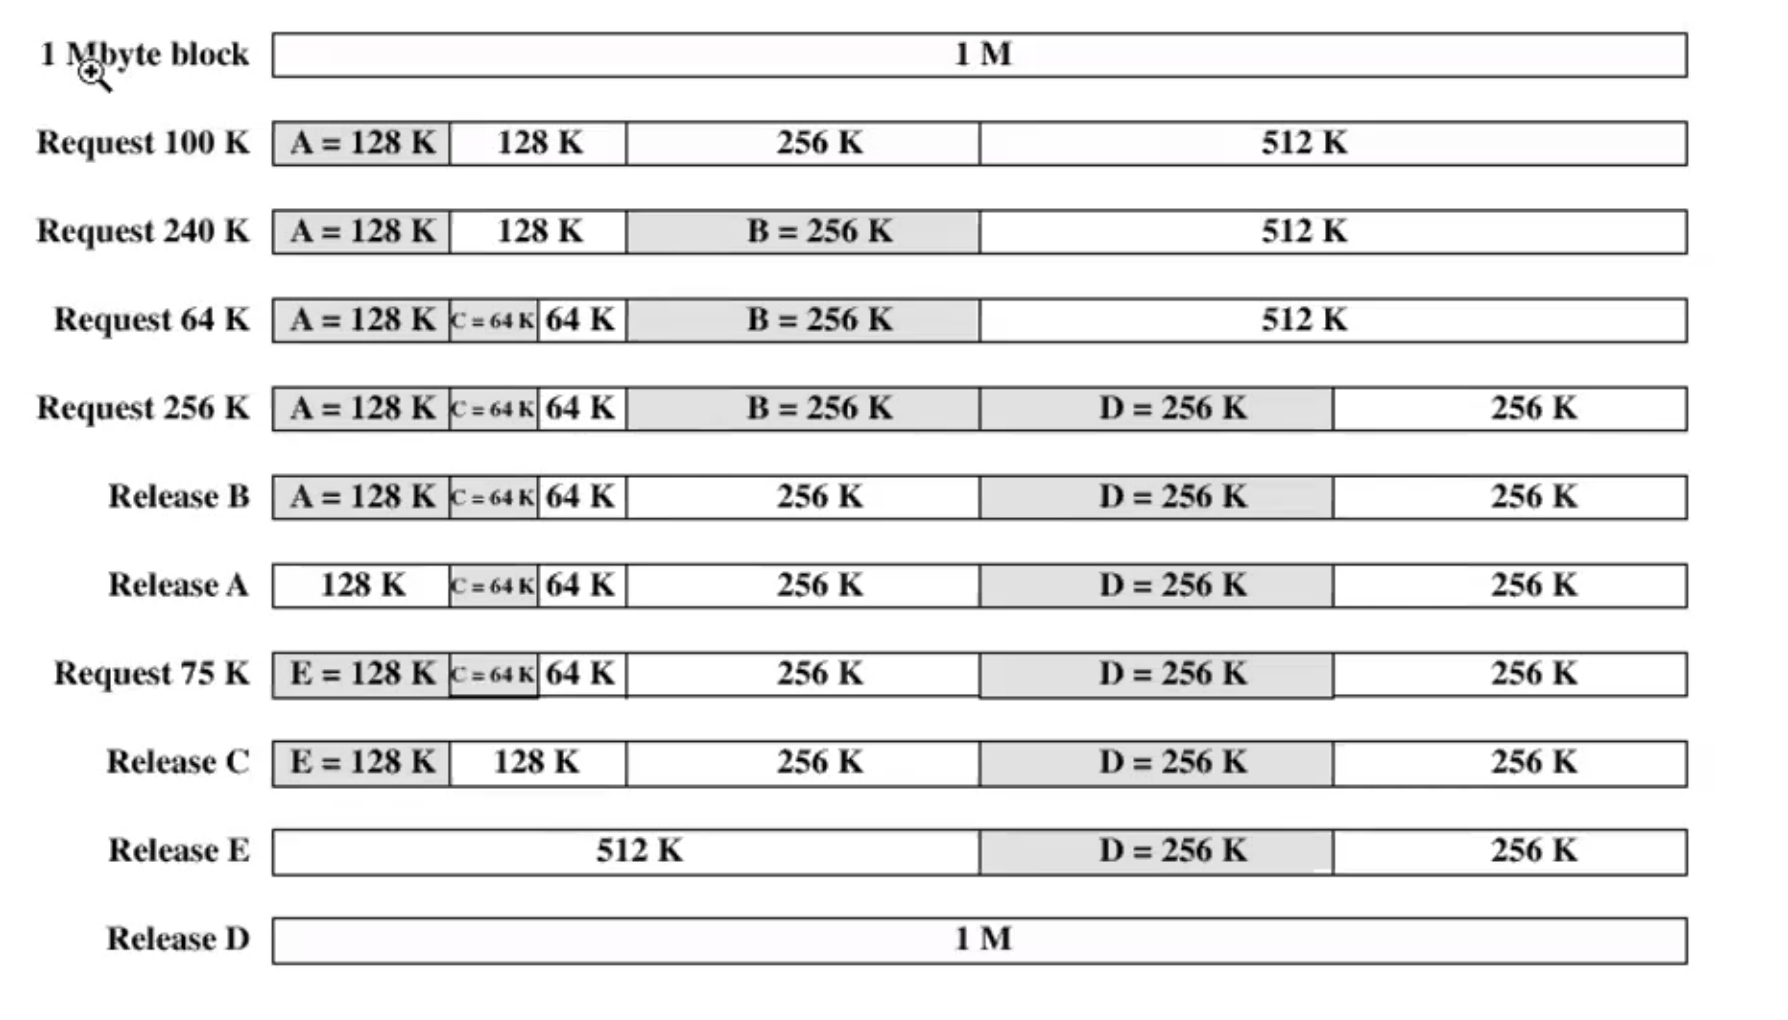
\includegraphics[scale=0.2]{buddy2}
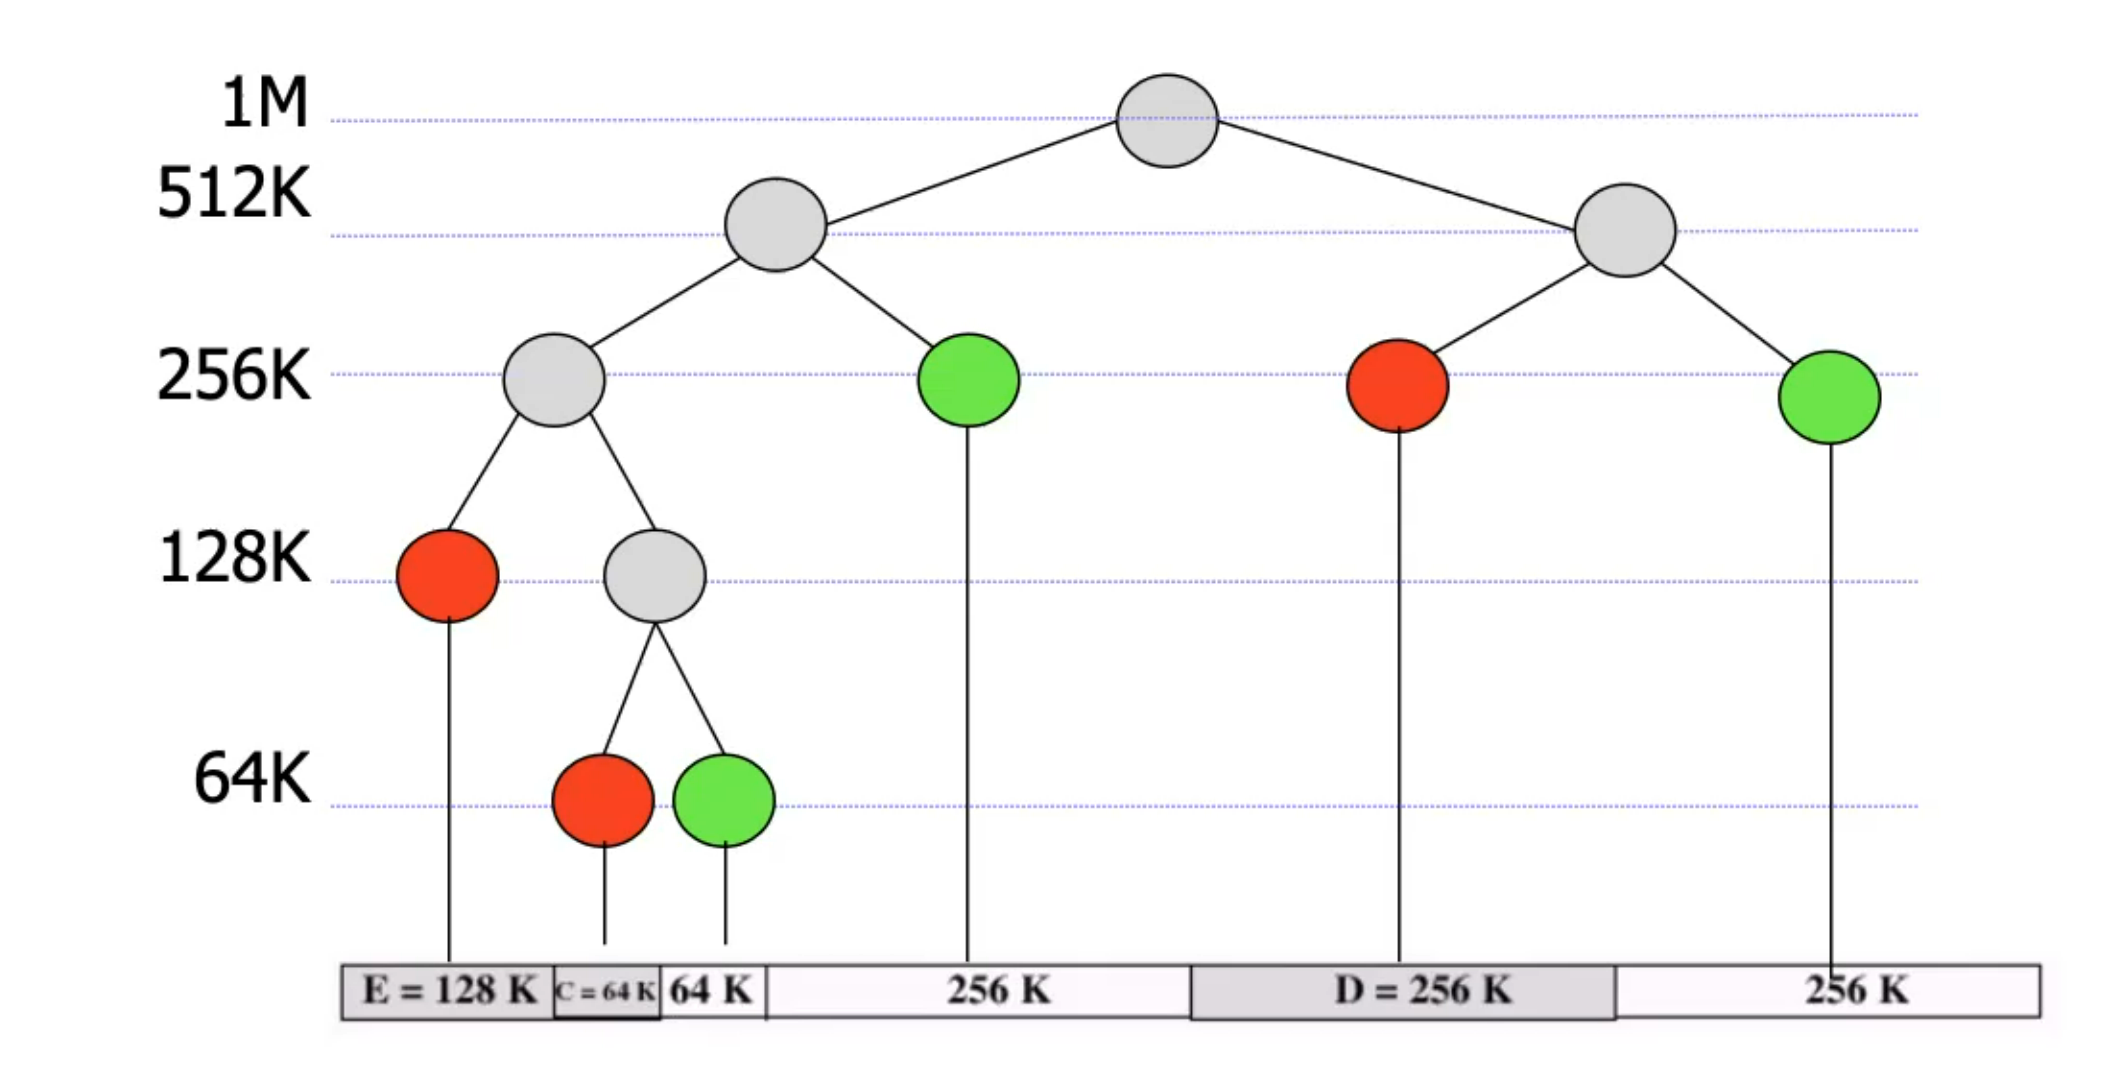
\includegraphics[scale=0.19]{buddy1}
\end{center}



% Riferimento libro pagg. 387 e seguenti 
\section{Paginazione}

La \emph{paginazione} \`e uno schema di gestione della memoria che consente allo spazio di indirizzamento fisico di un
processo di essere \textbf{non} contiguo, ovvero la memoria fisica pu\`o essere allocata dove disponibile. 
La paginazione permette di \emph{eliminare} la frammentazione esterna ed evita la necessit\`a di compattazione, due
problemi che affliggono l'allocazione din memoria contigua. L'implementazione della paginazione \`e frutto della
cooperazione tra il sistema operativo e l'hardware del computer.
\begin{itemize}
    \item \textbf{Memoria fisica:} viene divisa in blocchi detti \emph{frame} di dimensione fissa. (Tipicamente 512byte / 8kb).
\item \textbf{Memoria logica:} viene divisa in blocchi detti \emph{pagine}, di uguale dimensione dei \emph{frame}.
\end{itemize}
L'utilizzo di questa tecnica migliora l'\emph{efficacia} ma fa perdere di efficienza. Il sistema operativo avr\`a pi\`u compiti rispetto alle tecniche precedenti. 

Per eseguire un programma avente dimensione $n$ pagine, bisogna trovare $n$
frame liberi; per farlo si utilizza una tabella delle pagine (\emph{page table}) per mantenere traccia di quale frame corrisponde a quale pagina. 
Ci\`o significa che ogni processo ha una sua tabella delle pagine, che mappa
i frame del processo a cui appartiene. Inoltre, viene usata per tradurre 
un indirizzo logico in un indirizzo fisico. 

Durante l'esecuzione di un processo, l'accesso alla memoria, e di conseguenza la consultazione della tabella delle pagine, avviene pi\`u volte per istruzione (fetch, decode, execute, write back). In questo caso ogni
accesso alla memoria si traduce in due accessi, si ha quindi un peggioramento del $100\%$ rispetto al'allocazione 
contigua.

\subsubsection{Esempio di paginazione}

Supponiamo di avere delle pagine di dimensione 1KB e un programma di dimensione 2.3KB. Sono necessarie tre pagine,
e dell'ultima pagina si utilizzer\`a solo 0.3KB. Sperco: 0.7KB, \`e ancora possibile la \emph{frammentazione interna}, ma 
solo nell'ultima pagina.

\subsection{Traduzione degli indirizzi}

Quando si deve eseguire un processo si caricano le sue \emph{pagine} nei 
\emph{frame} disponibili, prendendole dalla memoria ausiliaria o dal file 
system. Questa idea fornisce grandi funzionalit\`a e ha diverse 
ramificazioni. Per esempio, lo spazio degli indirizzi logici \`e separato 
dallo spazio degli indirizzi fisici e dunque un processo pu\`o avere uno 
spazio degli indirizzi logici a 64 bit anche se il sistema ha meno di 
$2^{64}$ byte di memoria fisica. 

Ogni indirizzo generato dalla CPU \`e diviso in due parti: un \emph{numero 
di pagina (p)}  e un \emph{offset di pagina (d)}.
\begin{center}
\begin{tikzpicture}
\node at (2,0) [above] {numero di pagina};
\node at (6,0) [above] {offset di pagina};
\filldraw[color=black, fill=teal!80] (0,-1) rectangle ++(4,1);
\filldraw[color=black, fill=orange!80] (4,-1) rectangle ++(4,1);
\draw (4,-1) -- (4,1);
\node at (2,-0.25) [below] {$p$};
\node at (6,-0.25) [below] {$d$};
\end{tikzpicture}
\end{center}

\subsubsection{Sicurezza}

All'interno della tabella sono presenti dei bit relativi ai \emph{permessi}. Quando la CPU genera un'indirizzo, pu\`o 
essere per accedere ad un'istruzione, che dev'essere \emph{eseguibile}, oppure ad un dato, che non \`e eseguibile.
Vanno implementati meccanismi di \emph{checking}, solo le pagine che contengono codice eseguibile devono essere
eseguibili. Allo stesso modo per pagine in sola lettura: non deve essere possibile accedere in scrittura.
Viene anche tenuto conto se la pagina \`e stata modificata, per poterla salvare prima di cestinarla.

Nei sistemi operativi reali si hanno 5 o 6 livelli di paginazione.

% Lezione 03/04/2023
\subsubsection{Architettura MMU}

Il numero di pagina serve come indice per la tabella delle pagine relativa
al processo. La tabella delle pagine contiene l'indirizzo di base di 
ciascun frame nella memoria fisica e l'offset \`e la posizione nel frame a 
cui viene fatto riferimento. Perci\`o, l'indirizzo di base del frame viene 
combinato con l'offset della pagina per definire l'indirizzo di memoria 
fisica.

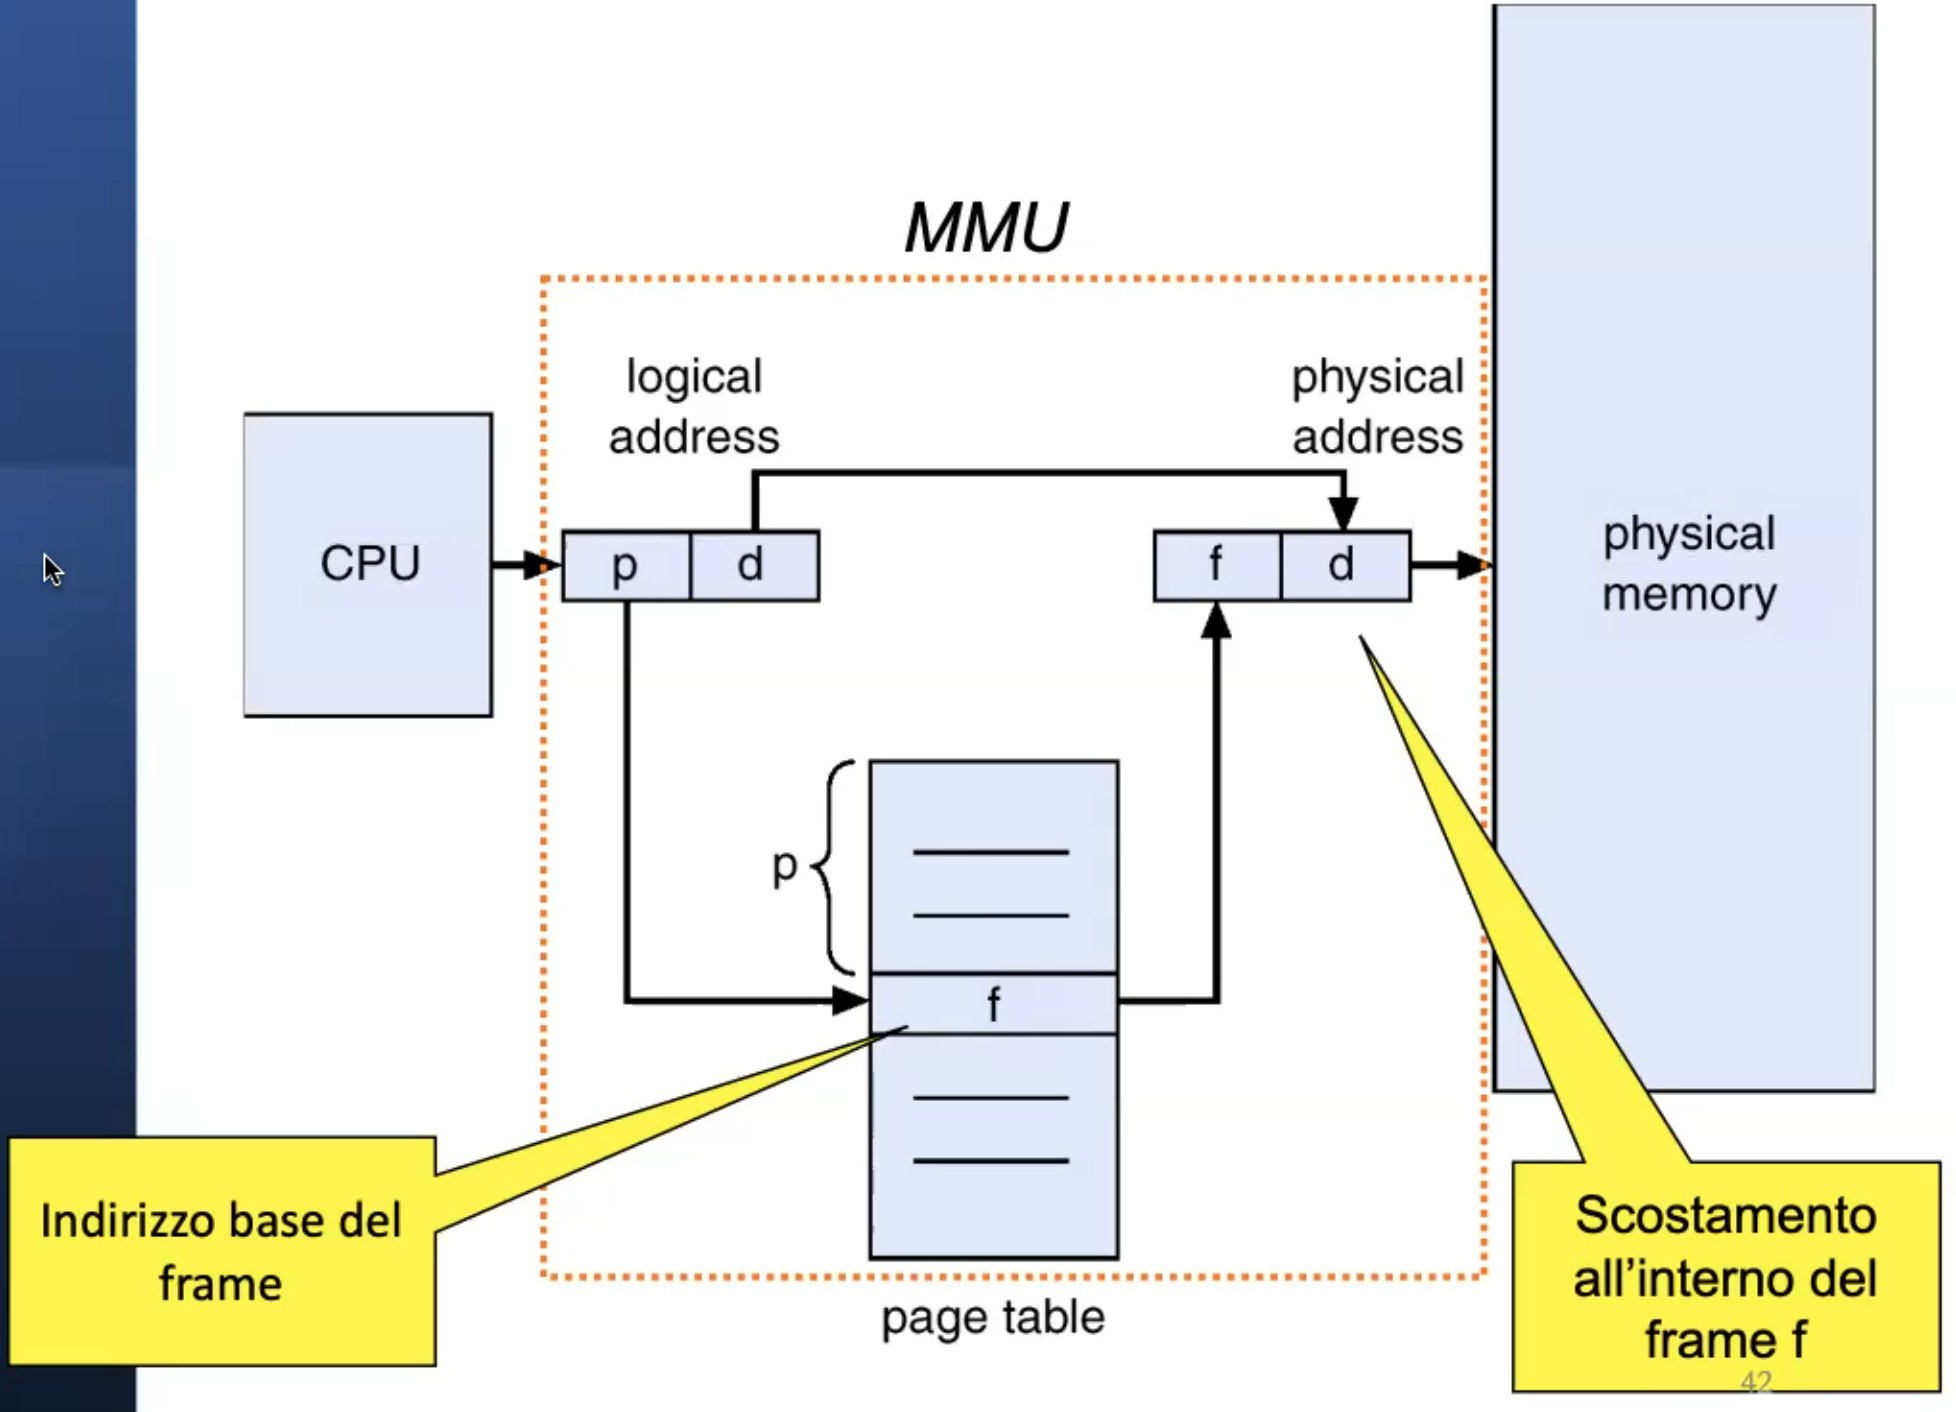
\includegraphics[scale=.2]{page_mmu}

I passaggi adottati dalla MMU per tradurre un indirizzo logico generato dalla CPU in un indirizzo fisico sono:
\begin{enumerate}
\item Estrarre il numero di pagina $p$ e utilizzarlo come indice nella tabella delle pagine.
\item Estrarre il numero di frame $f$ corrispondente dalla tabella delle pagine.
\item Sostituire il numero di pagina $p$ nell'indirizzo logico con il numero di frame $f$. 
\end{enumerate}

L'offset $d$ non cambia e pertanto non viene sostituito; il numero di frame e l'offset determinano insieme l'\emph{indirizzo fisico}.

La dimensione di una pagina \`e definita dall'hardware ed \`e una potenza di 2 compresa fra 4KB e 1GB, a seconda dell'architettura. Questo perch\'e semplifica la traduzione di un indirizzo logico nei corrispondenti numero di pagina e
offset di pagina. Ad esempio se la dimensione dello spazio degli indirizzi logici \`e $2^m$ e la dimensione di una pagina
\`e di $2^n$ parole/byte, allora gli $m-n$ bit pi\`u significativi di un indirizzo logico indicano il numero di pagina, e gli
$n$ bit meno significativi indicano l'offset di pagina. L'indirizzo logico ha quindi la forma seguente:

\begin{center}
\begin{tikzpicture}
\node at (2,0) [above] {numero di pagina};
\node at (6,0) [above] {offset di pagina};
\filldraw[color=black, fill=teal!80] (0,-1) rectangle ++(4,1);
\filldraw[color=black, fill=orange!80] (4,-1) rectangle ++(4,1);
\draw (4,-1) -- (4,1);
\node at (2,-0.25) [below] {$p$};
\node at (6,-0.25) [below] {$d$};
\node at (2, -1) [below] {$m - n$ bit};
\node at (6, -1) [below] {$n$ bit};
\node at (4,-1.7) [below] {num. pagine = $\frac{2^m}{2^n}$};
\end{tikzpicture}
\end{center}

\subsubsection{Esempio di traduzione degli indirizzi}

Supponiamo di avere una memoria da 8KB, suddivisa in 8 pagine (o \emph{frame}) da 1KB. Supponiamo anche di avere
un processo caricato in memoria composto da 4KB, ovvero 4 pagine. 
\begin{center}
\begin{tikzpicture}
% logical memory 
\filldraw[color=black, fill=lightgray!60] (0,3) rectangle ++(2,1);
\node at (1,3.5) {\texttt{page 0}};
\filldraw[color=black, fill=lightgray!60] (0,2) rectangle ++(2,1);
\node at (1,2.5) {\texttt{page 1}};
\filldraw[color=black, fill=lightgray!60] (0,1) rectangle ++(2,1);
\node at (1,1.5)  {\texttt{page 2}};
\filldraw[color=black, fill=lightgray!60] (0,0) rectangle ++(2,1);
\node at (1,0.5)  {\texttt{page 3}};

%page table
\filldraw[color=black, fill=white] (4,3) rectangle ++(0.75,0.75);
\node at (4.325,3.325) {\texttt{1}};
\filldraw[color=black, fill=white] (4,2.25) rectangle ++(0.75,0.75);
\node at (4.325,2.525) {\texttt{4}};
\filldraw[color=black, fill=white] (4,1.5) rectangle ++(0.75,0.75);
\node at (4.325,1.825)  {\texttt{3}};
\filldraw[color=black, fill=white] (4,0.75) rectangle ++(0.75,0.75);
\node at (4.325, 1.075)  {\texttt{7}};

% phisical memory
\filldraw[color=black, fill=white] (7,3) rectangle ++(2,1);
\filldraw[color=black, fill=lightgray!60] (7,2) rectangle ++(2,1);
\node at (8,2.5) {\texttt{page 0}};
\filldraw[color=black, fill=white] (7,1) rectangle ++(2,1);
\filldraw[color=black, fill=lightgray!60] (7,0) rectangle ++(2,1);
\node at (8,0.5)  {\texttt{page 2}};
\filldraw[color=black, fill=lightgray!60] (7,-1) rectangle ++(2,1);
\node at (8,-0.5)  {\texttt{page 1}};
\filldraw[color=black, fill=white] (7,-2) rectangle ++(2,1);
\filldraw[color=black, fill=white] (7,-3) rectangle ++(2,1);
\filldraw[color=black, fill=lightgray!60] (7,-4) rectangle ++(2,1);
\node at (8,-3.5)  {\texttt{page 3}};

% Arrows & Labels
\draw[->][color=gray!90] (2,0.5) -- (3.5,1.075) node [right][color=black] {\texttt{3}}; 
\draw[->][color=gray!90] (2,1.5) -- (3.5,1.825) node [right][color=black] {\texttt{2}}; 
\draw[->][color=gray!90] (2,2.5) -- (3.5,2.525) node [right][color=black] {\texttt{1}}; 
\draw[->][color=gray!90] (2,3.5) -- (3.5,3.325) node [right][color=black] {\texttt{0}}; 
\node at (1,0) [below] {\texttt{logical memory}};
\node at (4.325, 0.75) [below] {\texttt{page table}};
\node at (8, -4) [below] {\texttt{physical memory}};
% frame number and arrows
\node at (6.5, 3.5) [right] {\texttt{0}};
\draw[->][color=gray!90] (4.75,3.325) -- (6.5, 2.5) node[right][color=black] {\texttt{1}};
\node at (6.5, 1.5) [right] {\texttt{2}};
\draw[->][color=gray!90] (4.75,2.525) -- (6.5, -0.5) node[right][color=black] {\texttt{4}};
\draw[->][color=gray!90] (4.75,1.825) -- (6.5, 0.5) node[right][color=black] {\texttt{3}};
\node at (6.5, -1.5) [right] {\texttt{5}};
\node at (6.5, -2.5) [right] {\texttt{6}};
\draw[->][color=gray!90] (4.75,1.075) -- (6.5, -3.5) node[right][color=black] {\texttt{7}};
\end{tikzpicture}
\end{center}

L'indirizzo logico 936 corrisponde all'indirizzo fisico 1960. Per calcolarlo dobbiamo considerare la mappatura 
\texttt{pagina 0 $\to$ frame 1}. La pagina 0 del programma \`e mappata nella memoria fisica dall'indirizzo 1024 fino 
all'indirizzo fisico 2047. L'indirizzo fisico perci\`o diventa: \[1024 + \text{\texttt{offset}} = 1024 + 936 = 1960\]

\subsection{Tabella delle pagine}
Come detto in precedenza, gli accessi alla tabella delle pagine sono numerosi, quindi l'efficienza \`e fondamentale.
Idealmente, il metodo pi\`u veloce sarebbe quello di caricarla nei registri della CPU, ma questo dipende dalla 
dimensione della memoria: se la memoria \`e piccola, questa soluzione sarebbe applicabile ma allungherebbe i tempi
di context switch, perch\'e richiede il salvataggio dei registri. L'alternativa \`e quella di salvare la tabella delle pagine in
memoria, attraverso due metodi: il metodo della tabella delle pagine multilivello e il metodo della tabella delle pagine
invertita.

\subsubsection{Implementazione in memoria}

Con questa implementazione la tabella risiede nella meemoria. Vengono utilizzati due registri \texttt{PTBR}, (\emph{ page-table base register}) che punta alla tabella delle pagine, e il \texttt{PTLR}, (\emph{page-table length register}  opzionale) che contiene la dimensione della tabella delle pagine.
Il context-switch \`e pi\`u breve perch\'e richiede solo la modifica del \texttt{PTBR} e del \texttt{PTLR} (se presente).

\textbf{Problema:} Ogni accesso a dati/istruzioni richiede due accessi in memoria, uno per accedere alla tabella delle pagine e uno per accedere al dato/istruzione.
Questo problema pu\`o essere risolto tramite una cache veloce, e dedicata alla traduzine degli indirizzi, detta \emph{translation look-aside buffers (TLB)}. Il suo funzionamento prevede il confronto dell'elemento fornito con il campo chiave di tutte le \emph{entry} contemporaneamente. Il contenuto della cache non conterr\`a il dato, ma l'indirizzo fisico a cui esso \`e disponibile. 

Il TLB \`e molto costoso in termini di hardware. Nel TLB perci\`o, verr\`a memorizzato solo un piccolo sottoinsieme 
delle entry della tabella delle pagine, in riferimento alla localit\`a spazio-temporale. Inoltre, ad ogni context switch
il TLB viene ripulito per evitare mapping di indirizzi errati. 

\textbf{Accesso alla memoria:} se la pagina cercata \`e nel TLB, quest'ultimo restituisce il numero di frame con un
singolo accesso, con un $t. richiesto < 10\%$ del tempo richiesto in assenza di TLB. Altrimenti, \`e necessario accedere
alla tabella delle pagine in memoria. L'\emph{hit ratio} ($\alpha = \%$) \`e la percentuale delle volte in cui una pagina
si trova nel TLB. Si rende necessario definire il concetto di \emph{tempo di accesso effettivo}.

\subsubsection{Tempo di accesso effettivo - EAT}
Il tempo di accesso effettivo \`e dato dalla seguente formula:
\[ EAT = (T_{MEM} + T_{TLB}) \alpha + (2 T_{MEM} + T_{TLB})(1-\alpha) \]
dove:
\begin{itemize}
\item $T_{TLB}$ = tempo di accesso al TLB;
\item $T_{MEM}$ = tempo di accesso a memoria;
\end{itemize}

\subsubsection{Esempio}
\begin{itemize}
\item $T_{MEM} = 90 ns$; $T_{TLB} = 10 ns$; $\alpha = 90\%$;
\item $EAT = (90 + 10) * 0.9 + ((2 * 90) + 10) * (1 - 0.9) = 109 \approx 1.2 T_{MEM}$;
\end{itemize}

\subsubsection{Protezione}
La protezione viene realizzata associando \emph{bit di protezione} ad ogni frame/pagina. Alcuni esempi sono:
\begin{itemize}
    \item Bit di validit\`a: (\emph{valid-invalid bit}) per ogni entry della tabella delle pagine, se il bit \texttt{valid} \`e settato indica che la pagina associata \`e nello spazio di indirizzamento logico del processo; \texttt{invalid} indica che l'opposto.
\item Bit di accesso: serve ad indicare se una pagina modificabile o meno (read-only), se \`e eseguibile o no, eccetera.
\item Dirty-bit: indica se una pagina \`e stata modificata (sporcata) oppure no. Nel caso di dover rimuovere pagine dalla memoria, serve saperlo perch\'e le pagine modificate devono essere salvate.
\end{itemize}

\subsubsection{Condivisione}
Possono essere implementate anche tecniche di \emph{condivisione} del codice. In questo caso vi \`e un'unica
copia fisica (un unico \emph{frame}), ma pi\`u copie logiche (una per ogni processo). Il codice 
\emph{read-only} (rientrante) pu\`o essere condiviso tra processi (text editor, compilatori, window 
manager, ...); mentre i dati saranno, in generale, diversi da processo a processo.

\paragraph{Esempio:} tre istanze di un text editor avviate:
\begin{center}
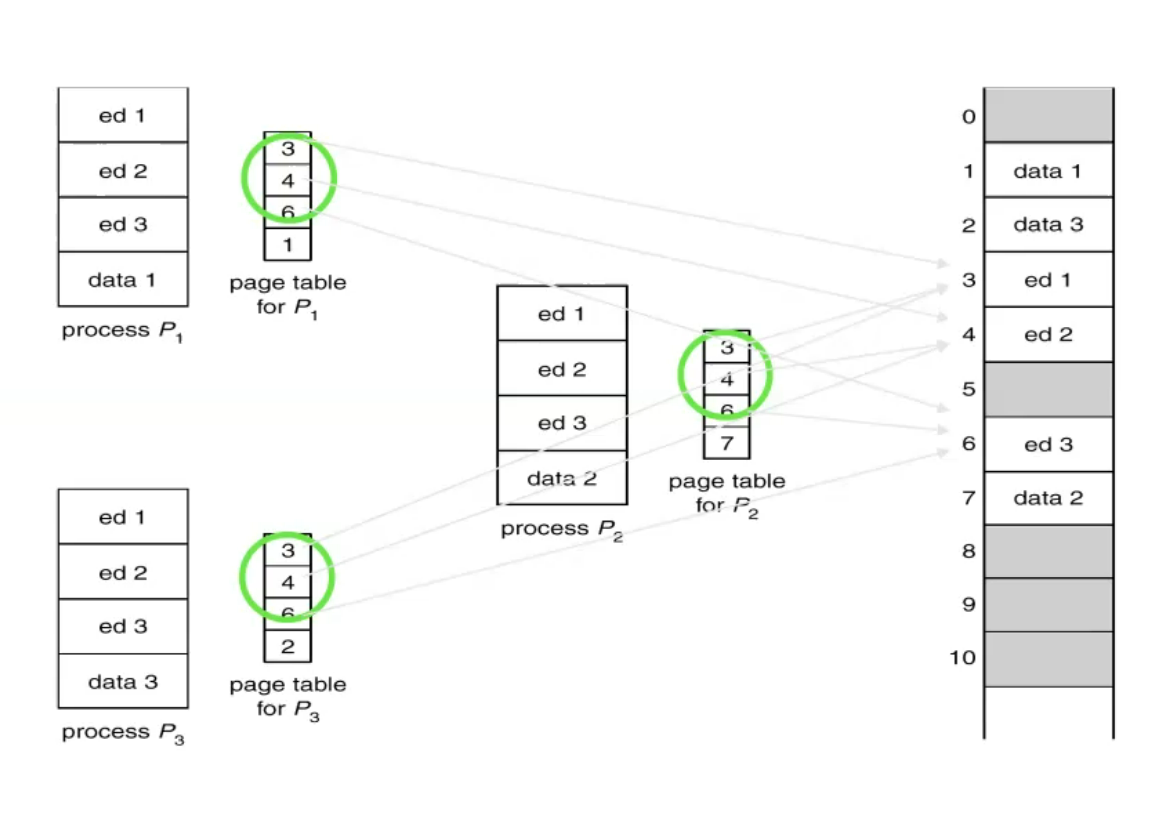
\includegraphics[scale=0.215]{share_code}
\end{center}
\subsubsection{Spazio di indirizzamento}

Considerando di avere uno spazio di indirizzamento virtuale di $2^{64}$, di molto maggiore dello spazio 
fisico. Ipotizzando di avere dei frame da 4KB, si otterrebbero che:
\[ |frame| = 4K = 2^{12} \to \frac{2^{64}}{2^{12}} = 2^{52} \approx 4.5 * 10^{15}\]
che equivalgono a circa $4.5*10^{52}$ entry (o righe) nella tabella delle pagine, per ogni processo.
Questo rende necessari dei meccanismi per gestire il problema della dimensione edlla tabella delle pagine:
\begin{itemize}
    \item Paginazione della tabella delle pagine $\to$ tabella delle pagine multilivello.
    \item Tabella delle pagine invertita.
\end{itemize}

\subsection{Paginazione multilivello}

Questa tecnica prevede che anche la tabella delle pagine sia \emph{paginata}. Solo alcune parti della 
tabella delle pagine sono memorizzate esplicitamente in memoria, le altre sono su disco. In questo modo non
\`e pi\`u necessario avere una zona di memoria contigua su cui mettere la tabella delle pagine. 
La parte di tabella presente in memoria sar\`a quella inerente alla localit\`a spazio-temporale.

\subsubsection{Paginazione a due livelli}
\begin{multicols}{2}
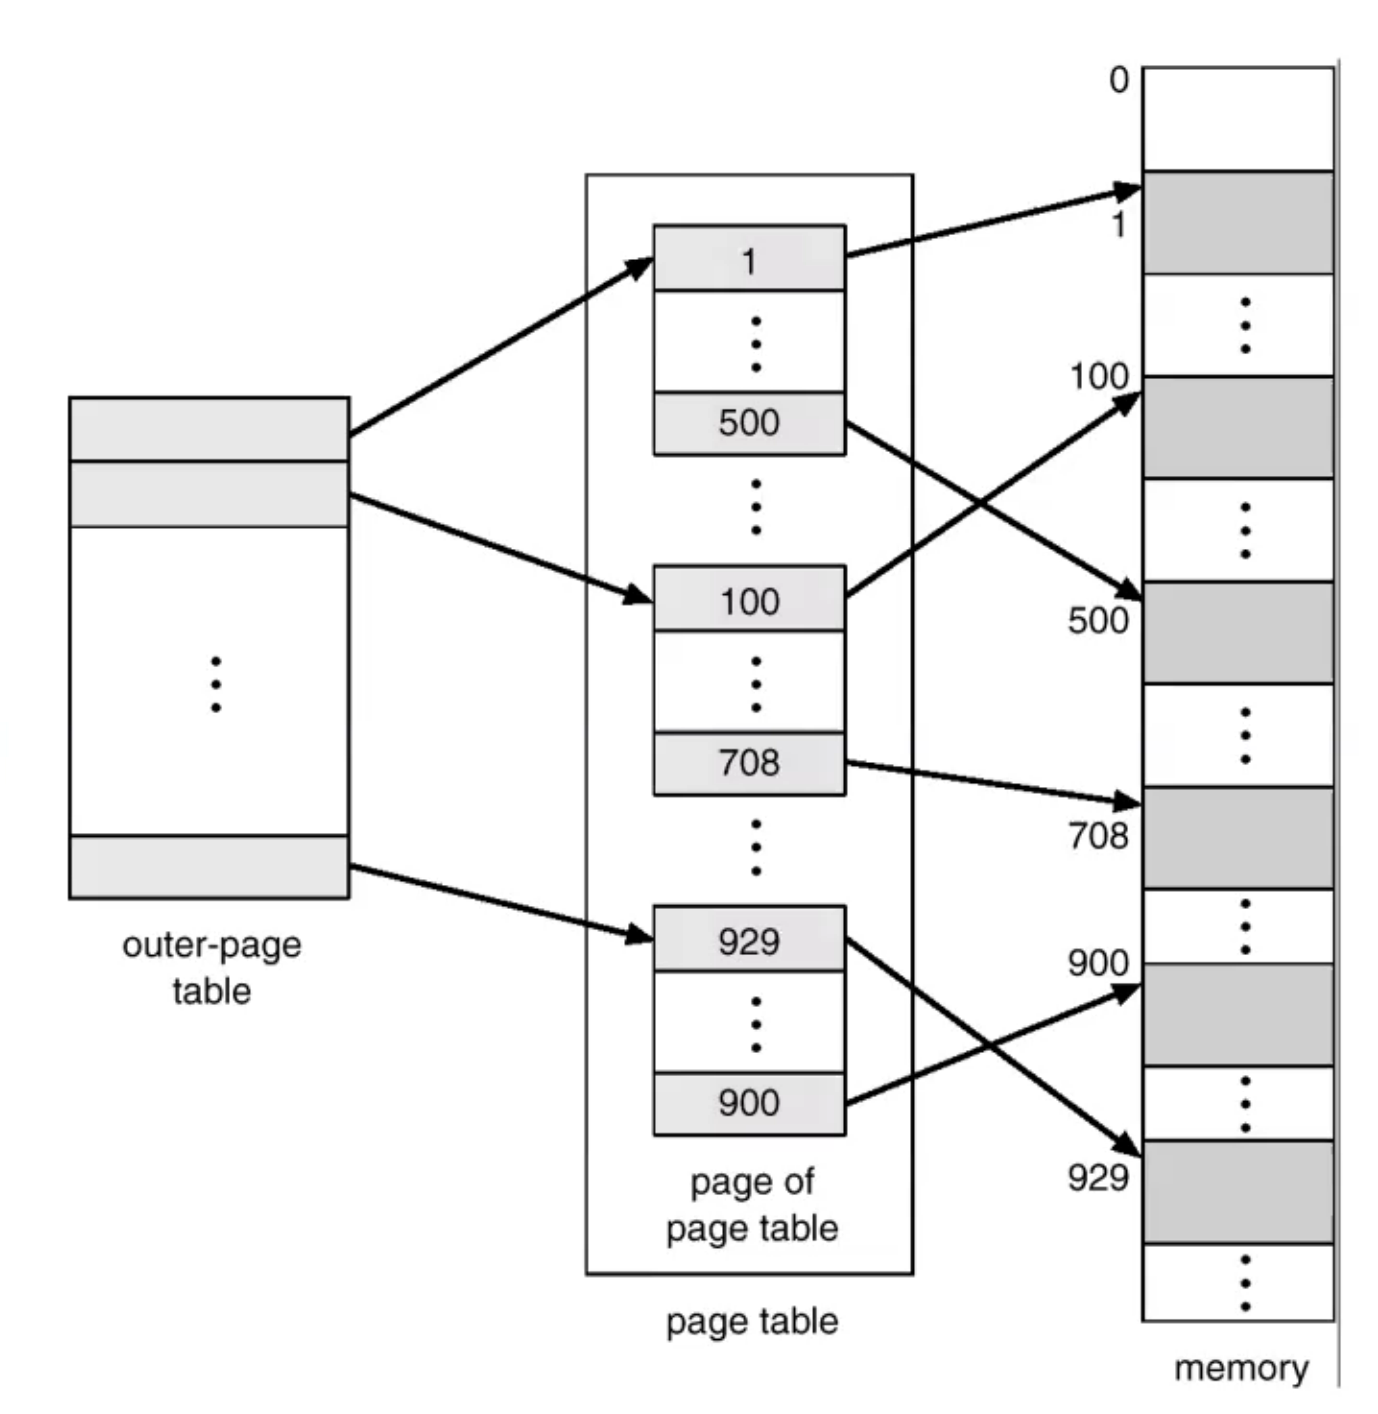
\includegraphics[scale=0.1]{2level}

Ora la tabella delle pagine punta a varie tabelle che a loro volta puntano ai frame in memoria. Se devo 
accedere al frame $100$, mi basta caricare in memoria la tabella delle pagine esterna e la pagina con la 
tabella inerente al frame di interesse. 
\end{multicols}
\subsubsection{Esempio}
Supponiamo di avere un indirizzo logico, generato dalla CPU, a 32bit. La dimensione di una pagina \`e di 
4KB = $2^{12}$. Di conseguenza avremo 12 bit di offset e 20 bit per il numero di pagina. 
\begin{itemize}
    \item p1: indice della tabella delle pagine esterna (10 bit).
    \item p2: offset all'interno della pagina della page table interna (10 bit). 
\end{itemize} 
\begin{center}
    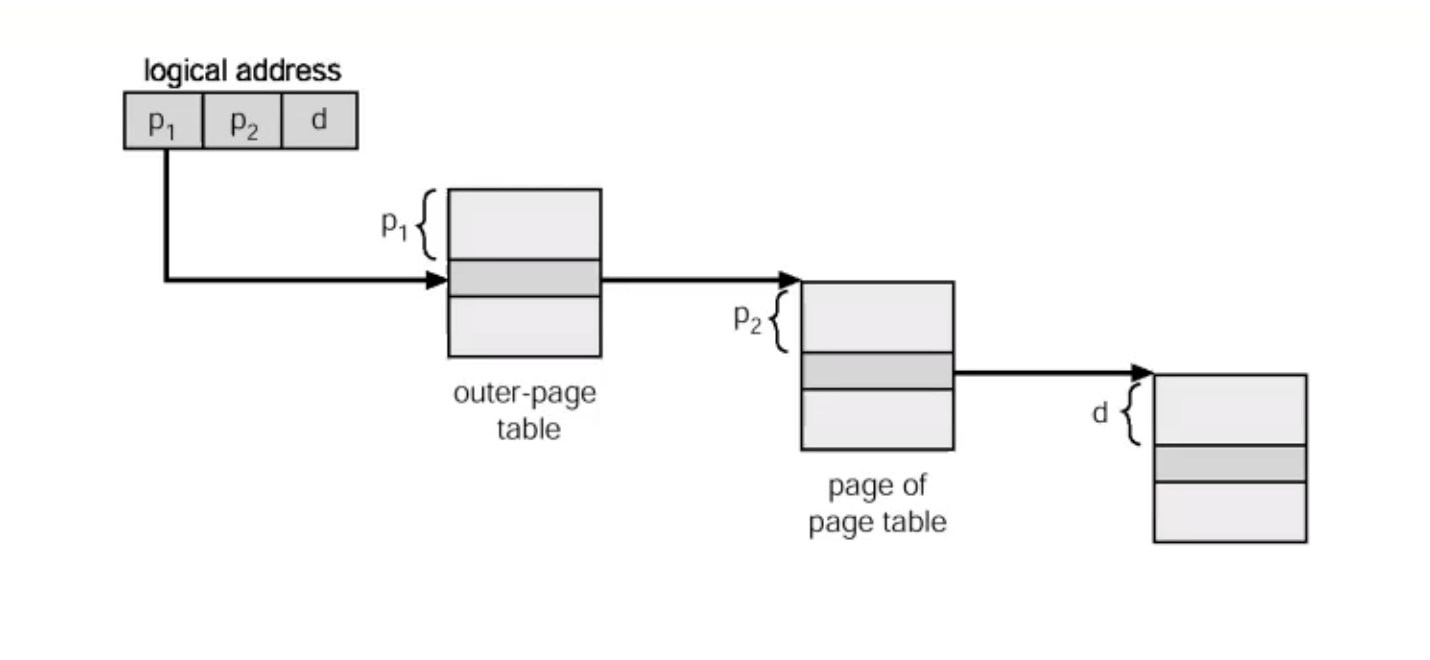
\includegraphics[scale=0.2]{multipag_example}
    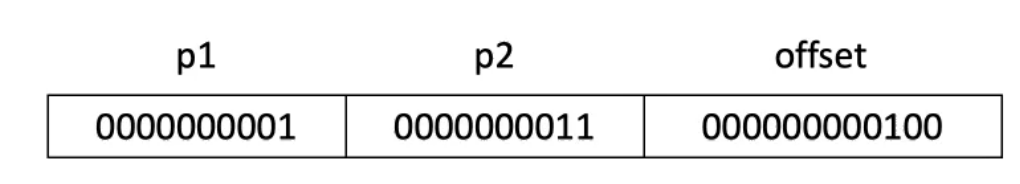
\includegraphics[scale=0.2]{index_example}
\end{center}
\begin{itemize}
    \item p1 = 1 $\to$ recupera la tabella di secondo livello corrispondente all'indirizzo indicato dalla 
        prima riga. 
    \item p2 = 3 $\to$ recupera l'indirizzo di terzo livello (\emph{l3}) indicato nella terza riga della tabella di 
        secondo livello. 
    \item offset = 4 $\to$ sommare al valore \emph{l3} fornito dalla tabella di secondo livello.
\end{itemize}

\subsubsection{Paginazione multilivello e prestazioni}
Ogni livello \`e memorizzato come una tabella separata in memoria. Supponendo una paginazione a tre livelli, la conversione dell'indirizzo logico in quello fisico pu\`o richiedere 4 accessi alla memoria. Il TLB 
mantiene comunque le prestazioni ragionevoli:
\begin{itemize}
    \item $T_{MEM} = 90ns$; $T_{TLB} = 10ns$; $\alpha = 90\%$.
    \item $EAT = (10 + 90) * 0.9 + (10+(4*90)) * 0.1 = 127ns \approx 1.4 T_{MEM}$.
\end{itemize}
\defbox{
Si ottiene una nuova formula per il calcolo dell'\emph{EAT}:
\[ EAT = \alpha (T_{MEM} + T_{TLB}) + ((n_{livelli}+1) * T_{MEM} + T_{TLB})(1 - \alpha)\]
}

\subsection{Tabella delle pagine invertita}

Questa tecnica permette di avere un'unica tabella delle pagine non paginata. La tabella \`e indicizzata per
ogni frame (pagina fisica), contenente:
\begin{itemize}
    \item Indirizzo virtuale della pagina che occupa quel frame.
    \item Informazioni sul processo che usa quella pagina.
\end{itemize}

Un problema conseguente a questa tecnica \`e dato dal fatto che, ad un dato indirizzo fisico, possono 
corrispondere pi\`u di un indirizzo virtuale. Di conseguenza \`e necessario cercare il valore desiderato. 
Vi \`e un aumento del tempo necessario per cercare un riferimento ad una pagina.
La ricerca non pu\`o essere sequenziale, la soluzione \`e l'utilizzo di una \emph{tabella hash}, che riduce
il tempo di ricerca da $O(n)$ ad $O(1)$.

In pratica, \`e necessario un meccanismo per la gestione delle collisioni, quando diversi indirizzi 
virtuali corrispondono allo stesso frame.

\subsubsection{Architettura MMU}
\begin{center}
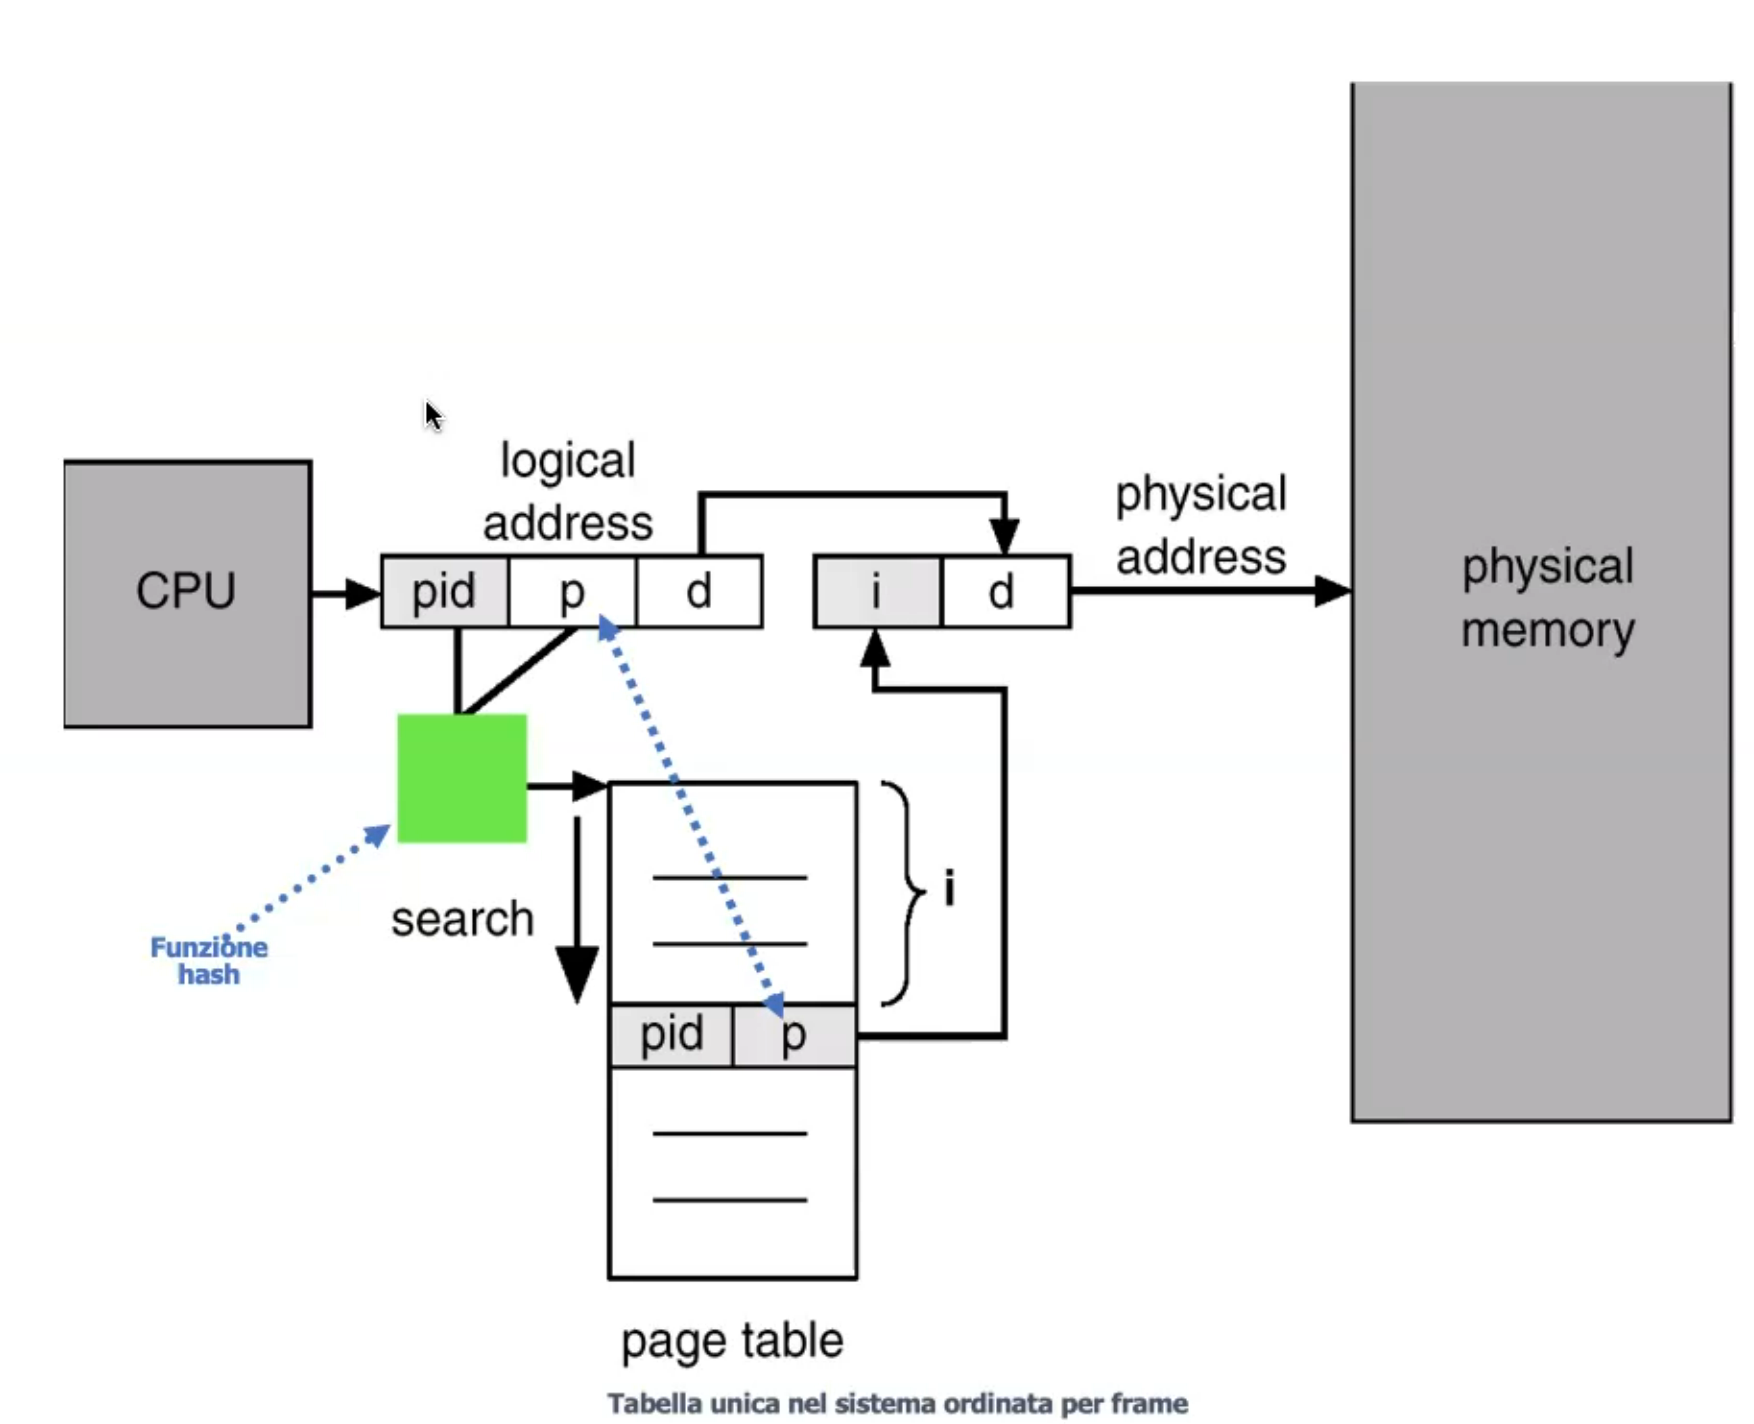
\includegraphics[scale=0.2]{hash_MMU}
\end{center}
Nel caso di un ambiente con poca dinamicit\`a questa tecnica \`e pi\`u conveniente; mentre nei sistemi 
general purpose \`e meglio la paginazione multilivello.

\section{Segmentazione}

Nella segmentazione non si distingue pi\`u pagina e frame, ma si parla di \emph{segmento} sia per 
quanto riguarda la memoria virtuale che per quella fisica.
Questo schema di gestione della memoria supporta la vista che l'utente ha della memoria, il programma 
 diventa una collezione di segmenti. Un segmento \`e un'unit\`a logica, costituita da un 
segmento per il main, un segmento per le procedure, uno per le funzioni, eccetera.
Ogni segmento \`e della dimensione perfetta per quello che deve contenere. Non ci sar\`a quindi 
frammentazione interna, ma ci sar\`a frammentazione esterna. 
\begin{center}
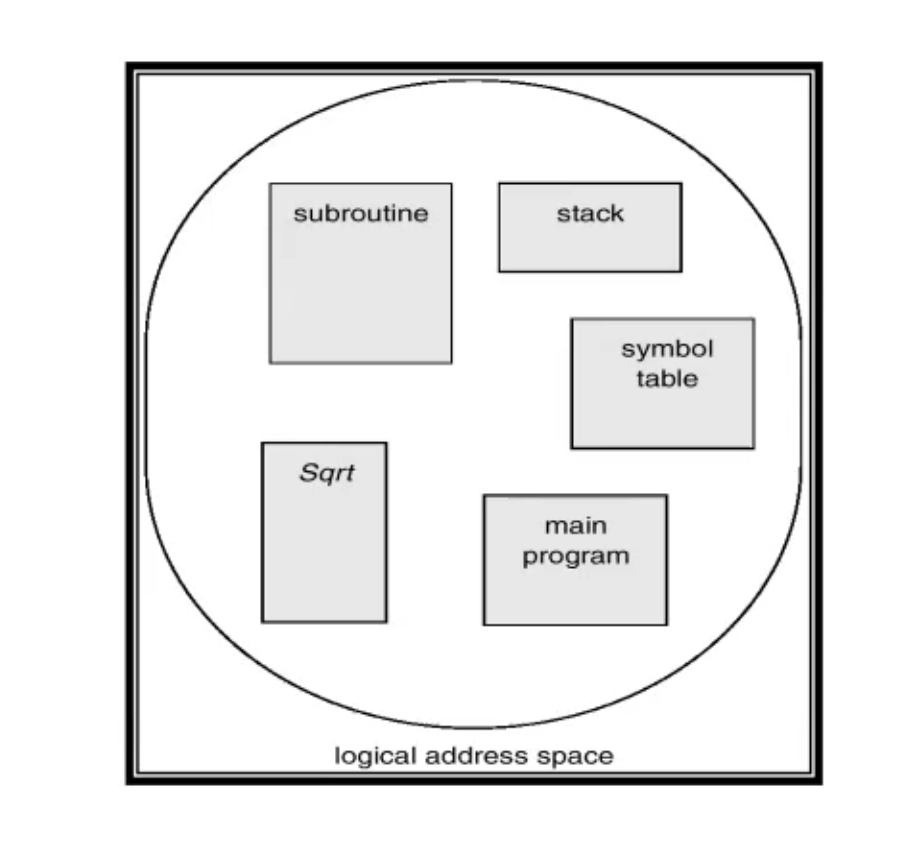
\includegraphics[scale=0.2]{segmentation1} 
\end{center}

\subsubsection{Vista logica}
\begin{center}
    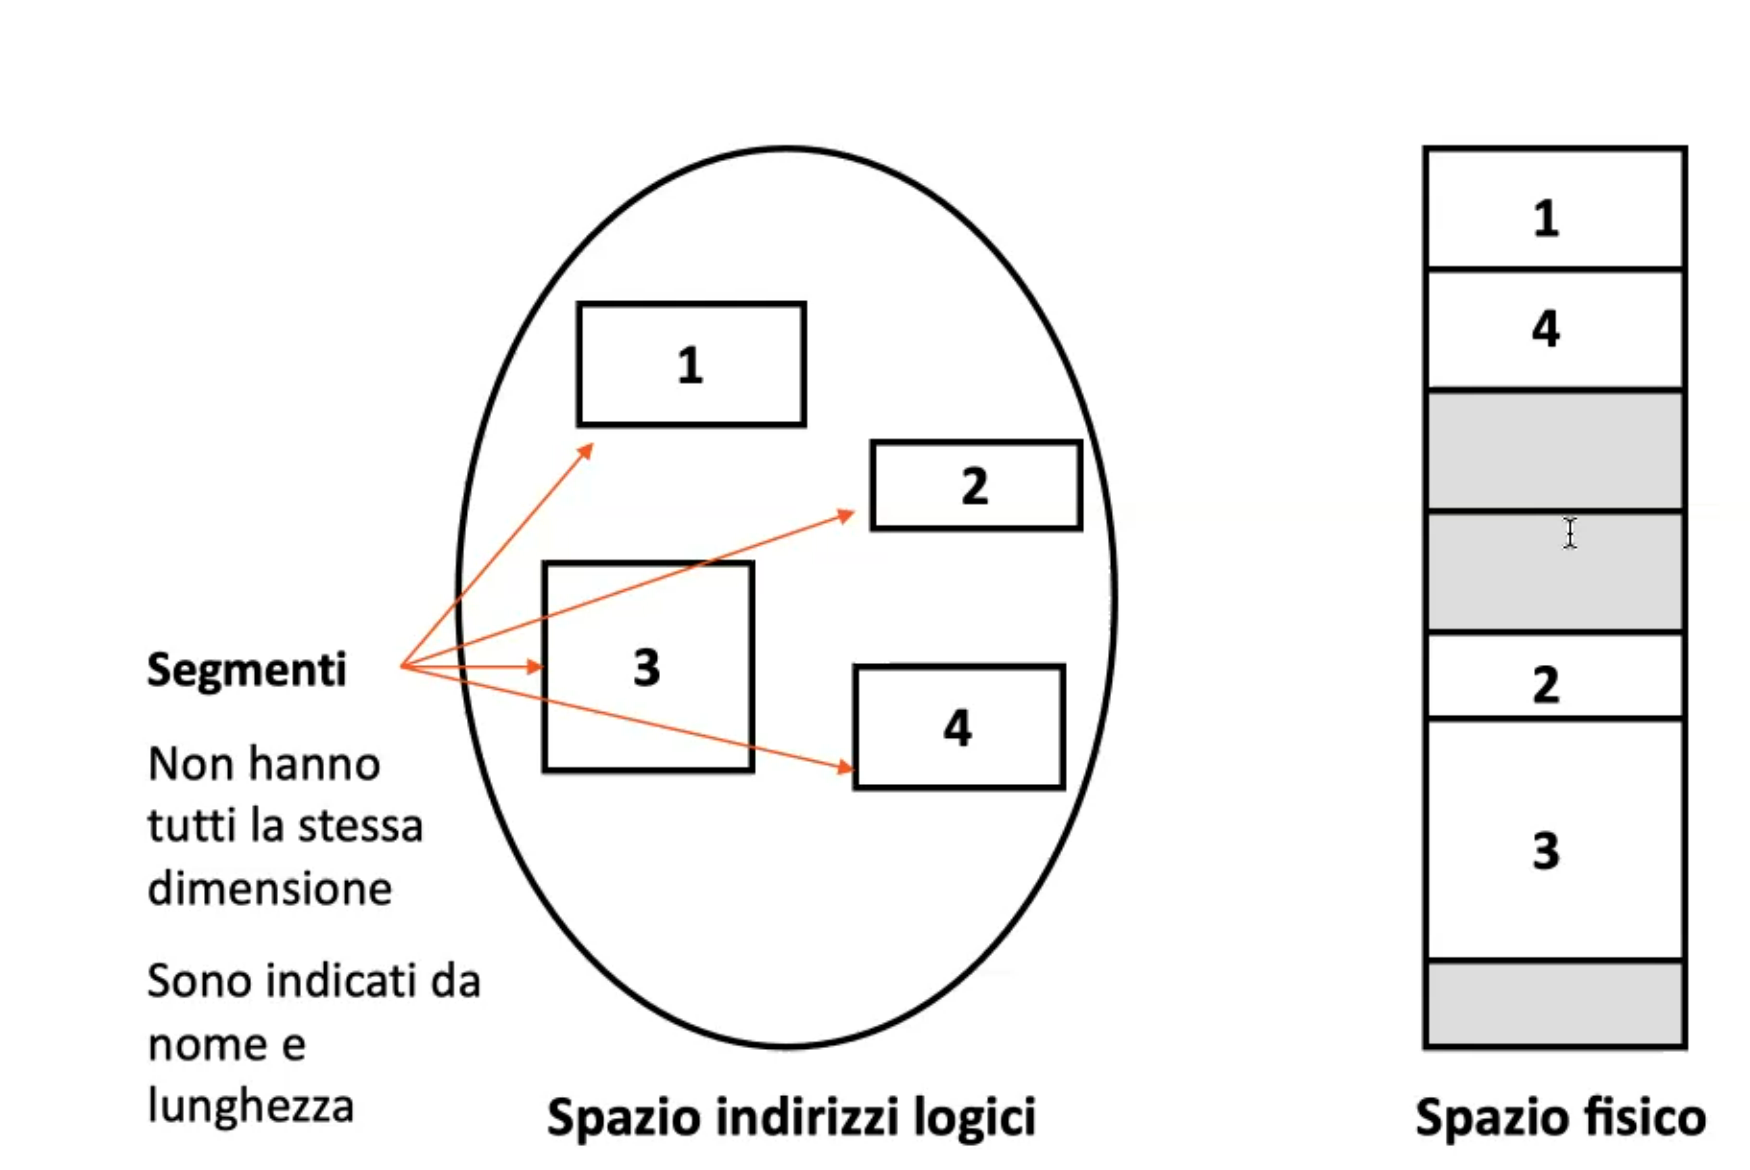
\includegraphics[scale=0.15]{segmentation2}
\end{center}

\subsection{Segmentation fault}
Ritorna il problema della frammentazione \emph{esterna}, perch\`e non si hanno pi\`u pagine/frame di 
uguale dimensione in cui posso mettere un segmento, ma si deve trovare lo spazio sufficientemente 
grande per contenere il segmento. Si ripete il problema della partizione continua con dimensioni 
variabili. 
L'MMU avr\`a una \emph{tabella dei segmenti} che mappa gli indirizzi logici bidimensionali in 
indirizzi fisici unidimensionali. Quando un indirizzo viene generato, si deve capire se 
quell'indirizzo pu\`o essere contenuto nel segmento. Ogni entry della tabella conterr\`a un'indirizzo 
\emph{base}, ovvero l'indirizzo fisico di partenza del segmento in memoria, e un valore \emph{limite},
che corrisponde alla lunghezza del segmento. Se l'indirizzo generato \`e maggiore avverr\`a un 
\emph{segmentation fault}.

\subsection{Tabella dei segmenti \& Architettura MMU} 
Sar\`a simile alla tabella delle pagine. In memoria avremo:
\begin{itemize}
    \item \defbox{\textbf{Segment-Table Base Register (SBTR)}: punta alla locazione della tabella dei 
        segmenti in memoria.}
    \item \defbox{\textbf{Segment-Table Length Register (SBLT)}: indica il numero di segmenti usati da
        un programma. Un indirizzo logico \texttt{<s,d>} \`e valido se $s < STLR$; mentre l'indirizzo 
        della tabella dei segmenti da recuperare \`e \texttt{STBR + s}.}
\end{itemize} 

\subsubsection{Architettura MMU}
\begin{center}
    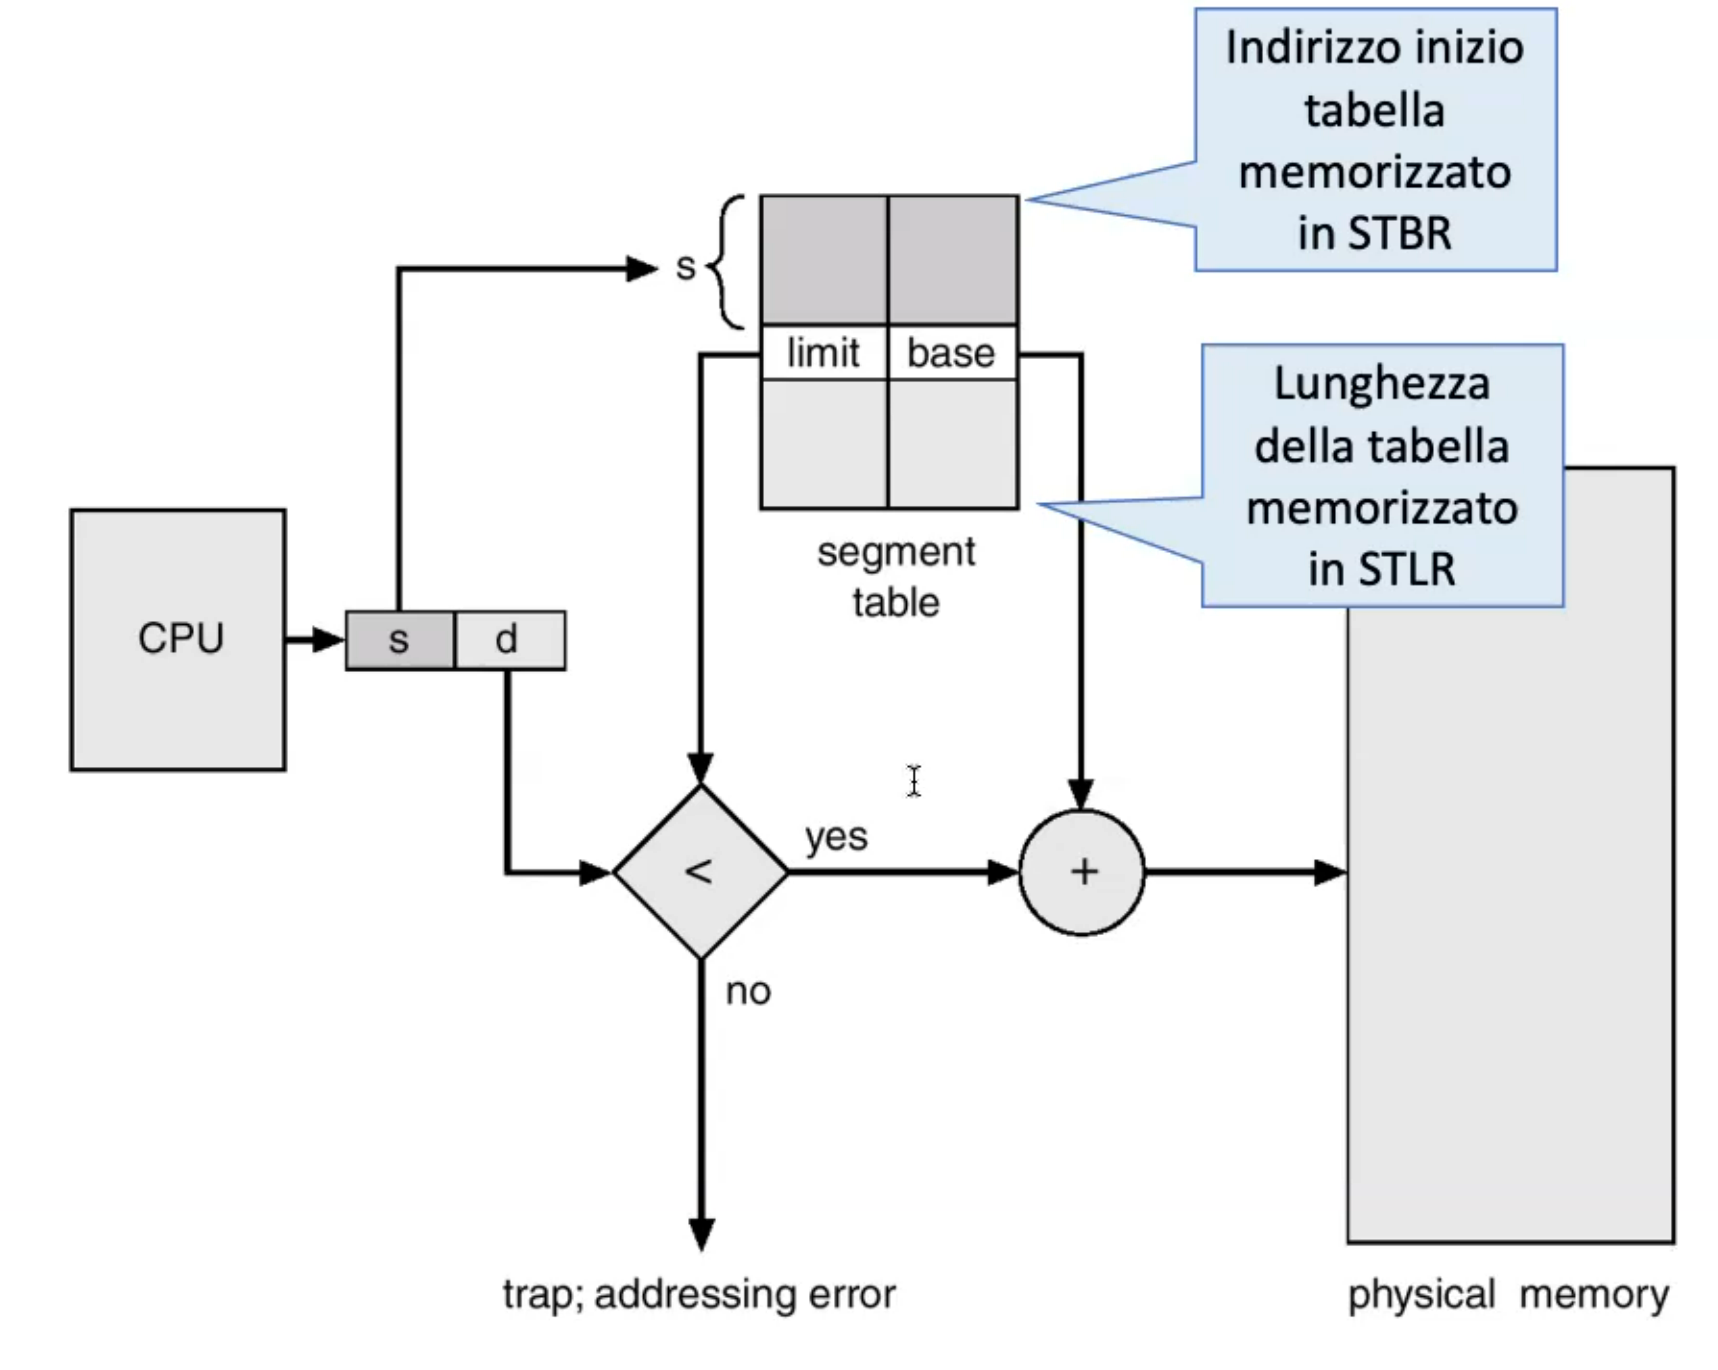
\includegraphics[scale=0.16]{mmu_seg}
\end{center} 

% Lezione 13/04 
\subsubsection{Esempio}

Ricordiamo che un segmento deve andare dove c'\`e abbastanza spazio per contenerlo, perch\'e non tutti 
i segmenti hanno la stessa dimensione.
\subsubsection{Tabella dei segmenti}
\begin{center}
    \begin{tabular}{c c c}
        \hline 
        \hline
        Segmento & Limite & Base \\
        \hline 
        \hline 
        0 & 600 & 219 \\
        \hline 
        1 & 14 & 2300 \\
        \hline
        2 & 100 & 90 \\
        \hline 
        3 & 580 & 1327 \\
        \hline
        \hline
    \end{tabular} 
\end{center}

Considerando l'indirizzo logico \texttt{<0, 430>}, abbiamo:
\begin{itemize}
    \item \texttt{segmento = 0}, \texttt{offset = 430}, verifichiamo che $430 < 600$.
    \item L'indirizzo fisico sar\`a calcolato come $430 + base_0 = 430 + 219 = 649$.
\end{itemize}

\subsection{Protezione \& Condivisione}
La segmentazione supporta naturalmente la protezione e la condivisione di porzioni di codice. Infatti,
ogni segmento \`e un'entit\`a con una semantica ben definita: segmento dati, segmento istruzioni, etc.

\subsubsection{Protezione}
Dal lato della protezione, ad ogni segmento sono associati dei \emph{bit di modalit\`a}, \texttt{read},
\texttt{write}, \texttt{execute}; inoltre, esiste un \texttt{valid bit}, che se \`e uguale a 0, sta 
ad indicare un segmento non legale, ovvero dice se il segmento \`e nello spazio di indirizzo del 
processo oppure no. Ad esempio, un tentativo di scrittura su un segmento \texttt{read-only} \`e 
facilmente riconosciuta e bloccata.

\subsubsection{Condivisione}
Per quanto riguarda la condivisione, basta inserirlo in un segmento. Questo rende possibile condividere 
anche parti di un programma, come le funzioni di libreria. 

\subsection{Segmentazione e frammentazione}
Il sistema operativo deve allocare spazio in memoria per tutti i segmenti di un programma che, avendo 
lunghezza variabile, vanno allocati attraverso tecniche dinamiche con \texttt{first-fit} o \texttt{best-fit}. Ma, per segmenti di dimensione significativa, ritorna la posssibilit\`a di frammentazione esterna.

\subsubsection{Paginazione}
\begin{center}
\defbox{\textbf{Vantaggi}
\begin{itemize}
    \item Non esiste frammentazione, se non minima interna.
    \item L'allocazione dei frame non richiede algoritmi specifici.
\end{itemize} 
\textbf{Svantaggi}
\begin{itemize}
    \item Separazione tra la vista utente e la vista fisica della memoria.
\end{itemize}
}
\end{center}
\subsubsection{Segmentazione}
\begin{center}
\defbox{\textbf{Vantaggi}
\begin{itemize}
    \item Consistenza tra vista utente e vista fisica della memoria. 
    \item Associazione di protezioni/condivisione ai segmenti.
\end{itemize}
\textbf{Svantaggi}
\begin{itemize}
    \item Richiesta allocazione dinamica dei segmenti. 
    \item Potenziale frammentazione esterna.
\end{itemize}
}
\end{center}


\newpage
\section{Segmentazione paginata}

La soluzione \`e quella di combinare le due strategie nella \emph{segmentazione paginata}. In questo 
modo si portano i vantaggi della segmentazione: separazione delle unit\`a logiche di un processo in 
segmenti diversi; poi, ogni segmento viene paginato. In questo modo si uniscono in una sola tecnica i 
vantaggi della segmentazione e quelli della paginazione. 

\begin{center}
    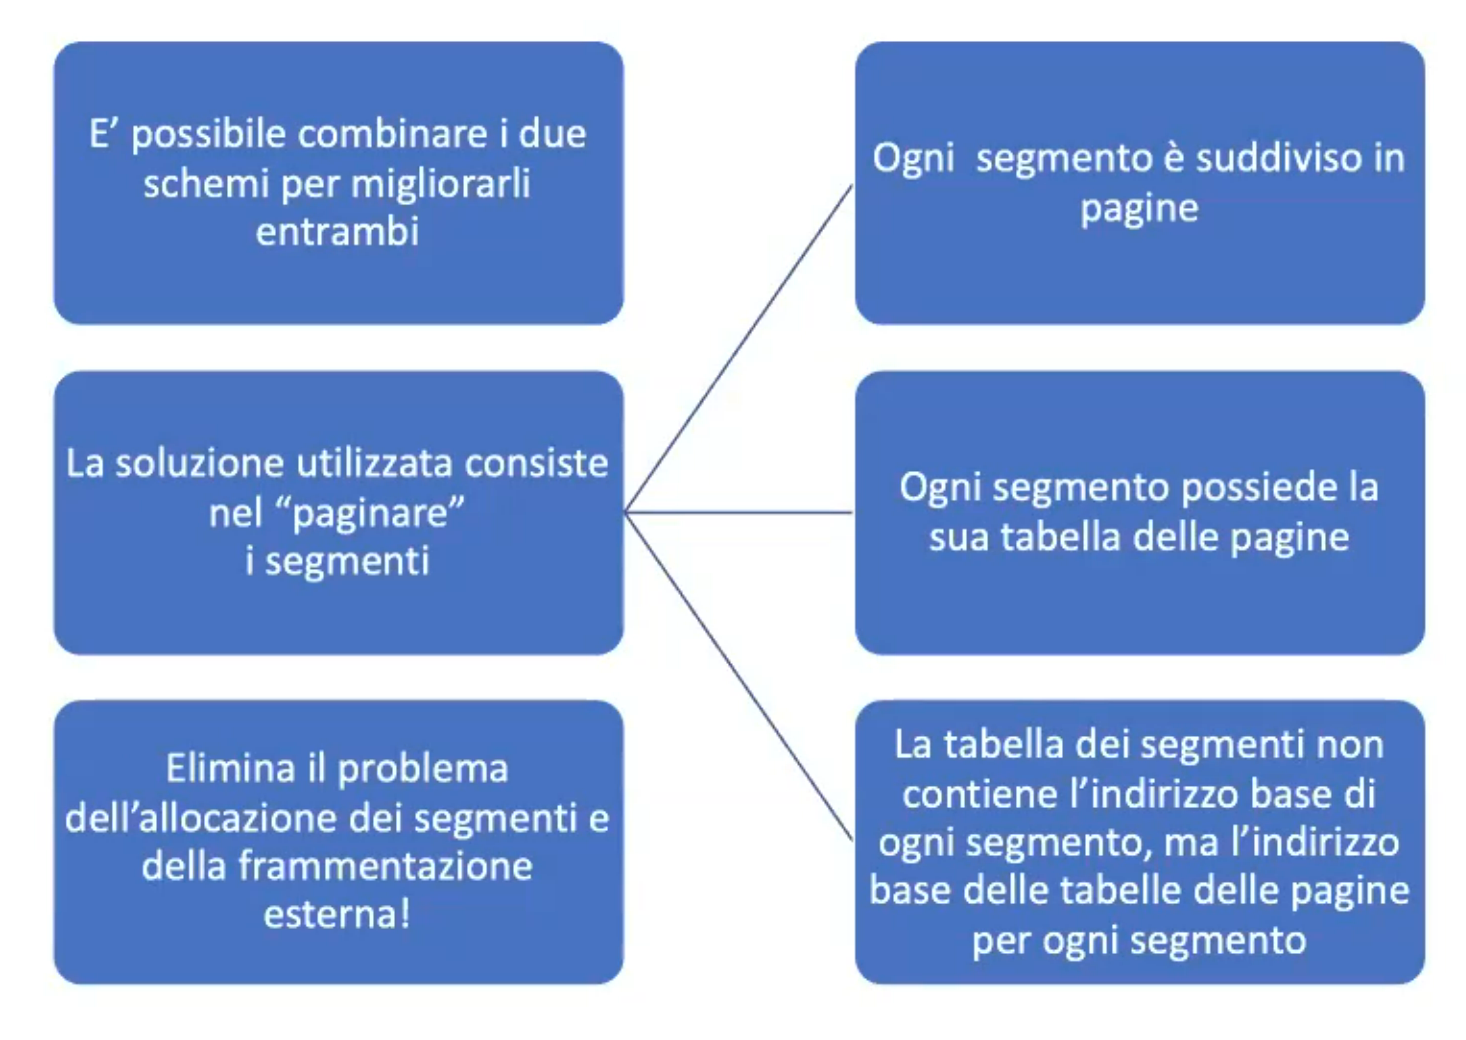
\includegraphics[scale=0.25]{seg_pag}
\end{center}

Con questa implementazione il \texttt{valid-bit} \`e a livello di pagina, mentre tutto quello che 
concerne la condivisione e la protezione \`e a livello di segmento. 

\newpage
\subsection{Architettura MULTICS}
L'archietettura di traduzione degli indirizzi si trasforma in qualcosa che combina le due strategie.
\begin{center}
    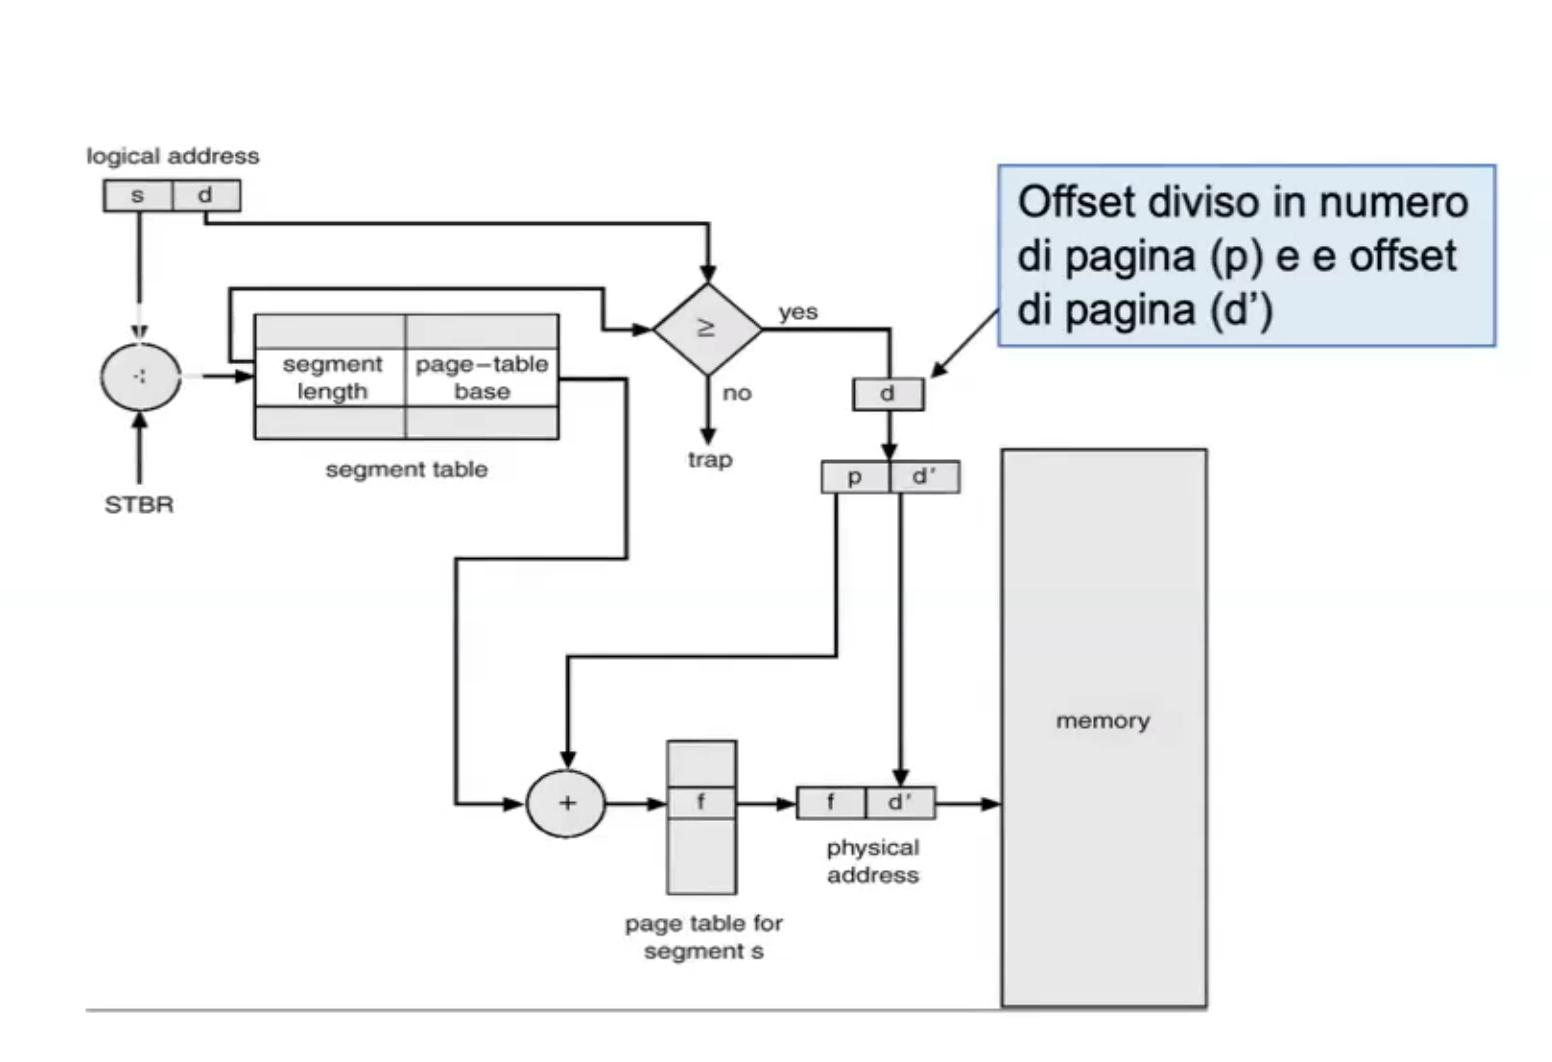
\includegraphics[scale=0.2]{multics}
\end{center} 

I passaggi necessari per ottenere l'indirizzo fisico diventano dunque:
\begin{enumerate}
    \item L'indirizzo logico generato dalla CPU \`e costituito da un \texttt{segmento} e un \texttt{offset}.
    \item Il segmento viene sommato al \texttt{segment-table base register}, in questo modo si accede 
        alla tabella dei segmenti corretta del processo. 
    \item All'interno della tabella dei segmenti si trovano due informazioni:
        \begin{enumerate}
            \item La \underline{lunghezza del segmento}, necessaria a verificare se l'offset non sta 
                all'interno del segmento. In caso contrario genera un \emph{segmentation fault}.
            \item Il \underline{page-table base register}, che assieme all'offset indicizza la pagina 
                associata al segmento. 
        \end{enumerate} 
    \item A questo punto si opera come avviene per la paginazione. L'offset viene diviso in due parti:
        il \emph{numero di pagina}(\texttt{p}), che indica il frame, e l'\emph{offset di pagina} 
        (\texttt{d'}, che associato al frame ottenuto precedentemente forma l'indirizzo fisico finale. 
\end{enumerate}

% Lezione di riferimento 13/04 
% Riferimento libro Silberschatz - Galvin Capitolo 10 - pagg. 419 e seguenti
\chapter{Memoria virtuale}

La \emph{memoria virtuale} \`e una tecnica che permette di eseguire processi che possono anche non essere
completamente contenuti in memoria. Il vantaggio principale offerto da questa tecnica \`e quello di 
permettere che i programmi siano pi\`u grandi della memoria fisica; inoltre, la memoria virtuale astrae 
la memoria centrale in un vettore di memorizzazione molto grande e uniforme, separando la memoria logica, 
vista dall'utente, da quella fisica. Questa tecnica libera i programmatori da problemi di limitazione 
della memoria. La memoria virtuale permette inoltre ai processi di condividere facilmente file e di 
realizzare memorie condivise, e fornisce un meccanismo efficiente per la creazione dei processi. 

Con la memoria virtuale tutto si sposta sul concetto di pagina, i segmenti, seppur presenti, sono ad un 
livello superiore. Il concetto chiave di questa strategia \`e la possibilit\`a di \emph{swappare} le 
pagine da e verso la memoria e non l'intero processo.

La memoria virtuale \`e molto pi\`u ampia della RAM perch\`e si appoggia ad un altro supproto di \underline{memoria secondario}, visto dalla CPU come RAM. (Es. HDD, SSD, nastri, ecc.). 

L'implementazione pu\`o avvenire in due modi: attraverso la \textbf{paginazione su domanda}, oppure 
attraverso la \textbf{segmentazione su domanda}. 


\subsection{Paginazione su domanda}

\subsubsection{Principio}
\defbox{Una pagina viene caricata in memoria solo quando necessario.
In questo modo si occupa meno RAM, lasciando pi\`u posto per altri processi e di conseguenza permettendo 
un livello di multiprogrammazione pi\`u elevato. Inoltre, l'avvio di un processo avviene pi\`u rapidamente. Diventa fondamentale sapere lo stato in cui si trova ogni pagina di un processo, il \texttt{valid-bit} 
indicher\`a se la pagina \`e in RAM o no.}

\subsubsection{Schema concettuale} 

\begin{center}
    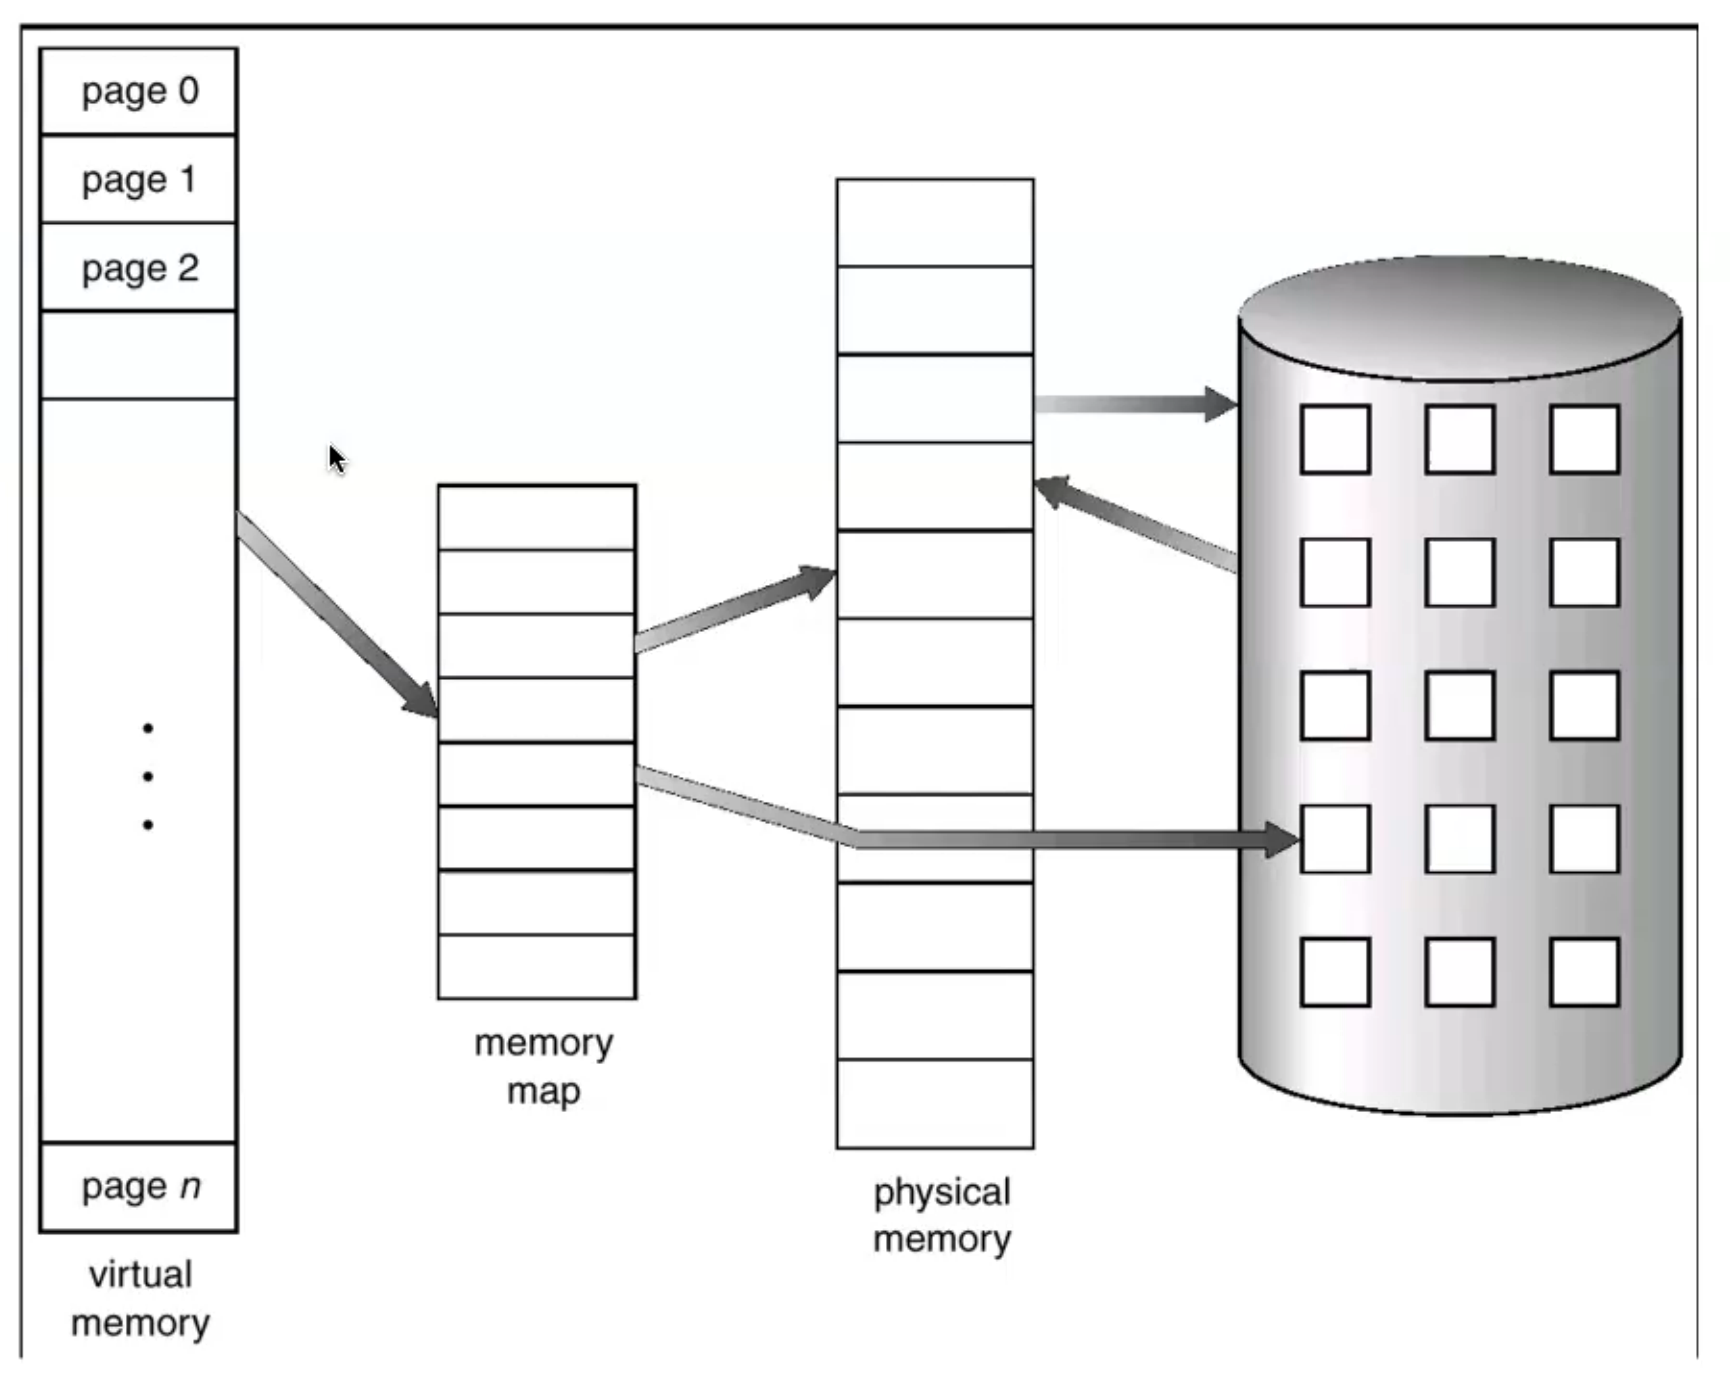
\includegraphics[scale=0.2]{concept_virtmem}
\end{center}
Quando la CPU genera un indirizzo virtuale che \`e mappato su disco, il sistema operativo si occupa di 
trasferire il frame in memoria e scambiarlo con un altro se la memoria \`e gi\`a piena. 

\subsubsection{Page fault}
Lo stato di una pagina \`e dato dal \texttt{validity bit}, se il bit $= 0$, la pagina non \`e in 
memoria, se il bit $= 1$, la pagina \`e in memoria. Inizialmente tutti i bit saranno a $0$. 
Il \emph{page fault} avviene quando, durante la traduzione di un indirizzo logico in un indirizzo fisico,
una entry ha un bit di validit\`a a $0$.
\begin{center}
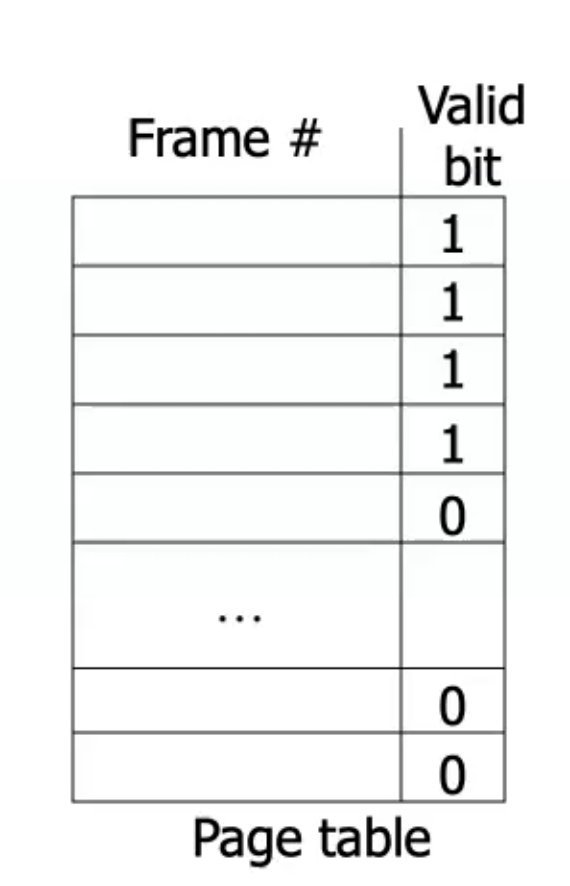
\includegraphics[scale=0.15]{page_table_fault}
\end{center} 

\subsubsection{Gestione dei Page Fault}
Il page fault causa un'interrupt al sistema operativo, che agisce come segue:
\begin{enumerate}
    \item Il sistema operativo verifica una tabella (associata al processo); se il riferimento non \`e 
        valido, uccide il processo. Se il riferimento \`e valido, attiva il caricamento della pagina.
    \item Cerca un \underline{frame vuoto}. 
    \item Swap della pagina nel frame (dal disco). 
    \item Modifica le tabelle, imposta a $1$ il \texttt{valid bit} della page table e nella tabella 
        interna al processo la pagina \`e in memoria. 
    \item Ripristina l'istruzione che ha causato il page fault. 
\end{enumerate} 
\subsubsection{Esempio}
\begin{center}
    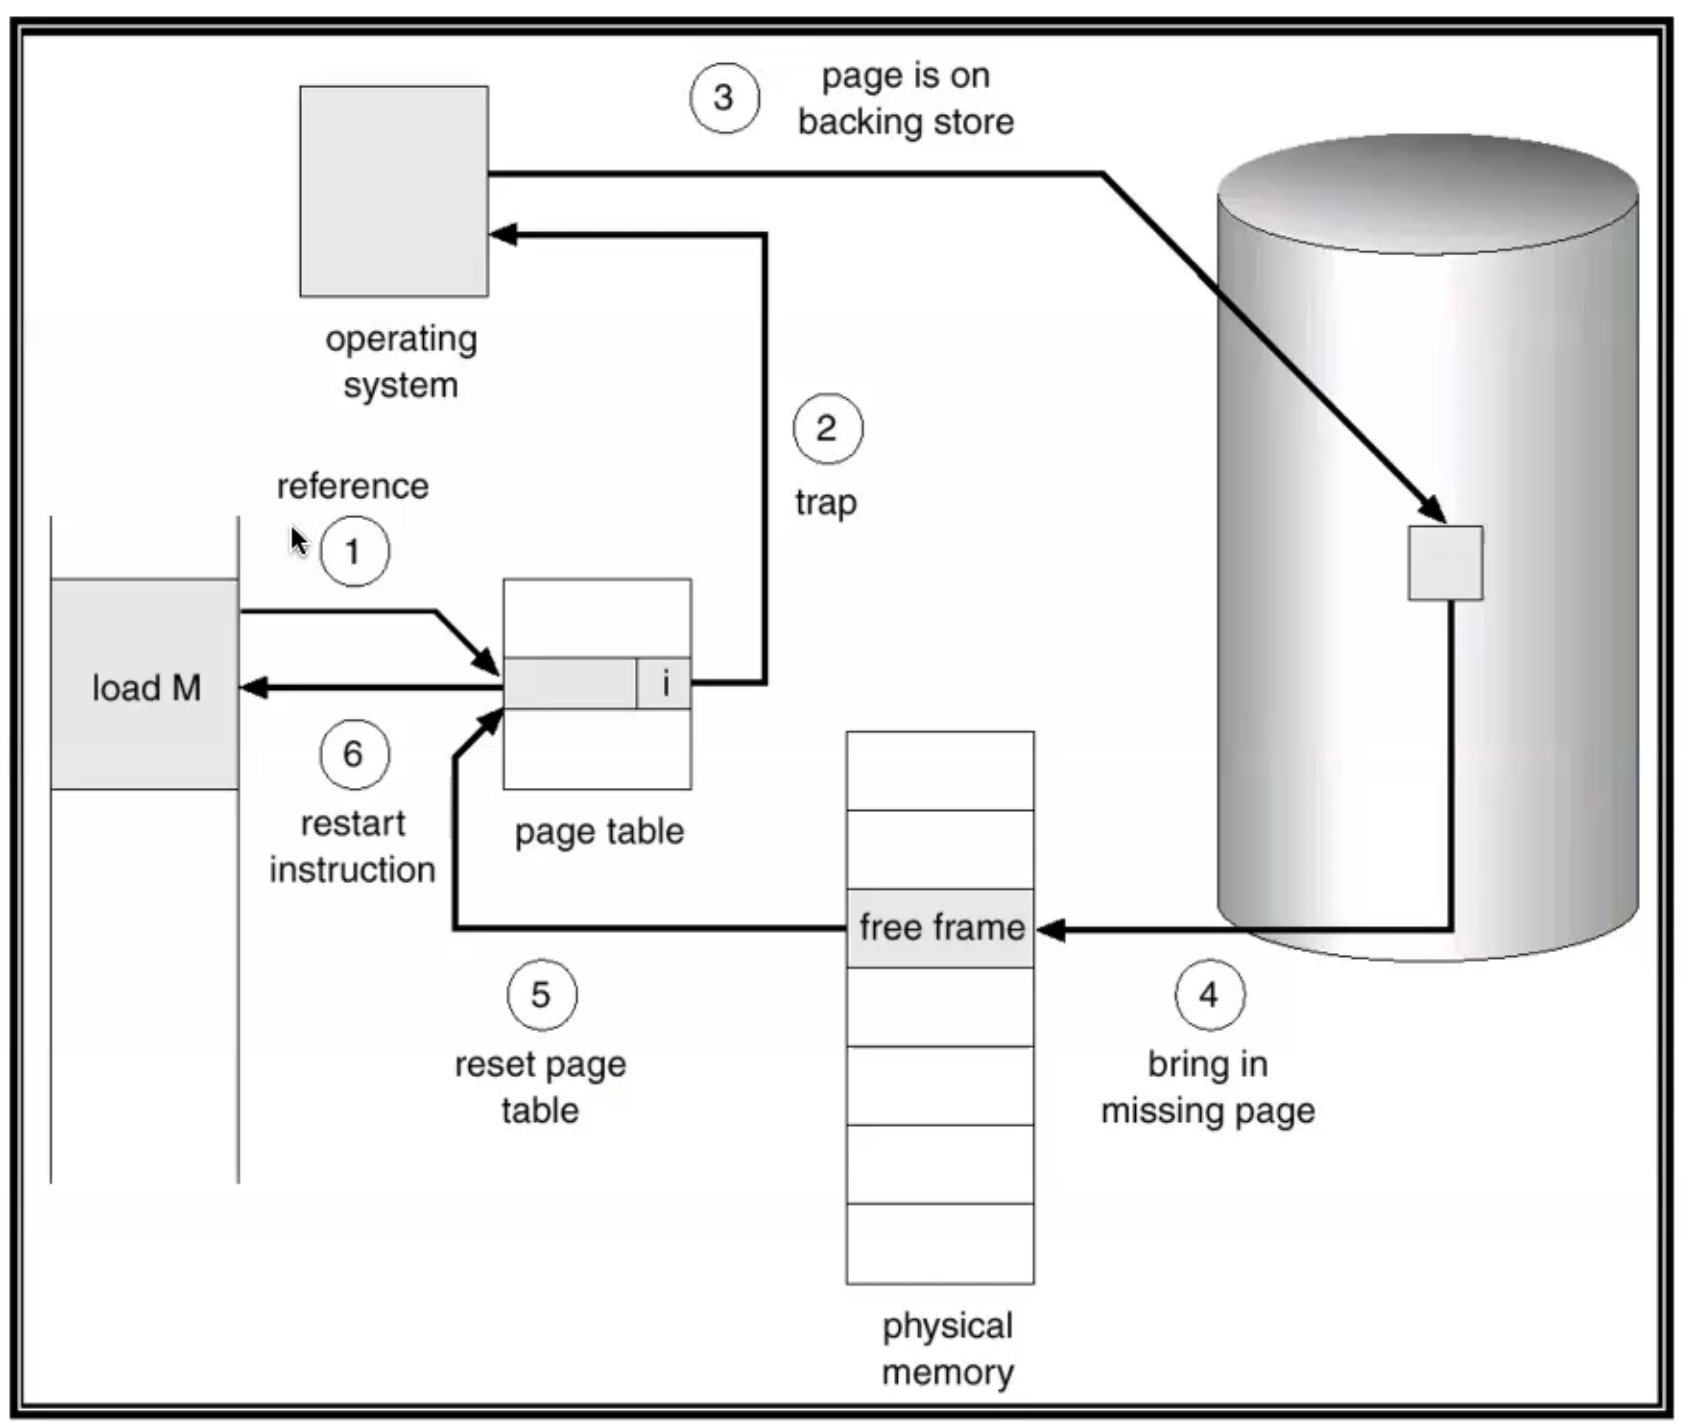
\includegraphics[scale=0.2]{pagefault_manage}

    \tiny{$i =$ invalid ($= 0$).}
\end{center} 

\subsection{Prestazioni}

\subsubsection{Impatto su EAT}
La paginazione su domanda influenza il tempo di accesso effettivo alla memoria. Il tasso di page fault 
\`e compreso tra 0 e 1. ($0 < p < 1$). Se $p = 0$, nessun page fault si \`e verificato; se $p = 1$, ogni 
accesso \`e un page fault.

\defbox{La formula per il calcolo dell'EAT diventa perci\`o: 
\[ EAT = (1 - p) * t_{mem} + p * t_{page\_fault} \]
dove $t_{mem}$ \`e strettamente legato alla strategia di allocazione della memoria.}

Se, ad esempio, si sta usando la paginazione, $t_{mem}$ sar\`a:
\[ t_{mem} = \alpha (T_{TLB} + T_{MEM}) + (1 - \alpha)(T_{TLB} + (N+1)T_{MEM}) \]

\subsubsection{Costo del page fault} 
Il tempo di page fault \`e dato da tre componenti principali:
\begin{itemize}
    \item \underline{Servizio dell'interrupt}: il costo dell'interrupt routine. 
    \item \underline{Swap in}: il costo della lettura da disco verso la memoria.
    \item \underline{Costo del riavvio del processo}.
    \item \underline{Swap out}: opzionale.
\end{itemize}

\subsubsection{Esempio}
Supponiamo di avere $t_{mem} = 100ns$; $t_{page\_fault} = 1ms (= 10^6ns)$. Calcoliamo EAT. 
\[ EAT = (1 - p) * 100 + p * 10^6 = 100 - 100*p + 1000000*p = 100*(1 + 9999 p)ns \]

Per mantenere il peggioramento entro il $10\%$ rispetto al tempo di accesso standard, si deve avere 
$p < 0.0001 \approx 10^{-4}$. Infatti:
\[ 100 * (1.1) > 100 * (1 + 9999p) \Rightarrow p < 0.0001\]
Ovvero, si deve mantenere un rateo di 1 page fault ogni 10000 accessi. \`E fondamentale mantenere basso 
il livello di page fault: questo peggioramento si somma con il peggioramento gi\`a presente (del $20\%$) 
per la gestione della paginazione. 

\subsection{Rimpiazzamento delle pagine}

La percentuale di peggioramento dipende da cosa accade quando le pagine in memoria devono essere rimpiazzate. L'obbiettivo \`e quello di minimizzare il numero di page fault attraverso un \emph{algoritmo} opportuno. 

La gestione del page fault si trasforma come segue: 
\begin{enumerate}
    \item Il sistema operativo verifica una tabella (associata al processo); se il riferimento non \`e 
        valido, uccide il processo. Se il riferimento \`e valido, attiva il caricamento della pagina.
    \item \defbox{Cerca un \underline{frame vuoto}. Se esiste, salta al punto 4. Se \textbf{non esiste}, usa un 
        algoritmo di rimpiazzamento delle pagine per scegliere la "\emph{vittima}".}
    \item Swap della vittima su disco. 
    \item Swap della pagina nel frame da disco. 
    \item Modifica le tabelle (page table, bit di validit\`a). 
    \item Ripristina l'istruzione che ha causato il page fault. 
\end{enumerate}

\begin{center}
    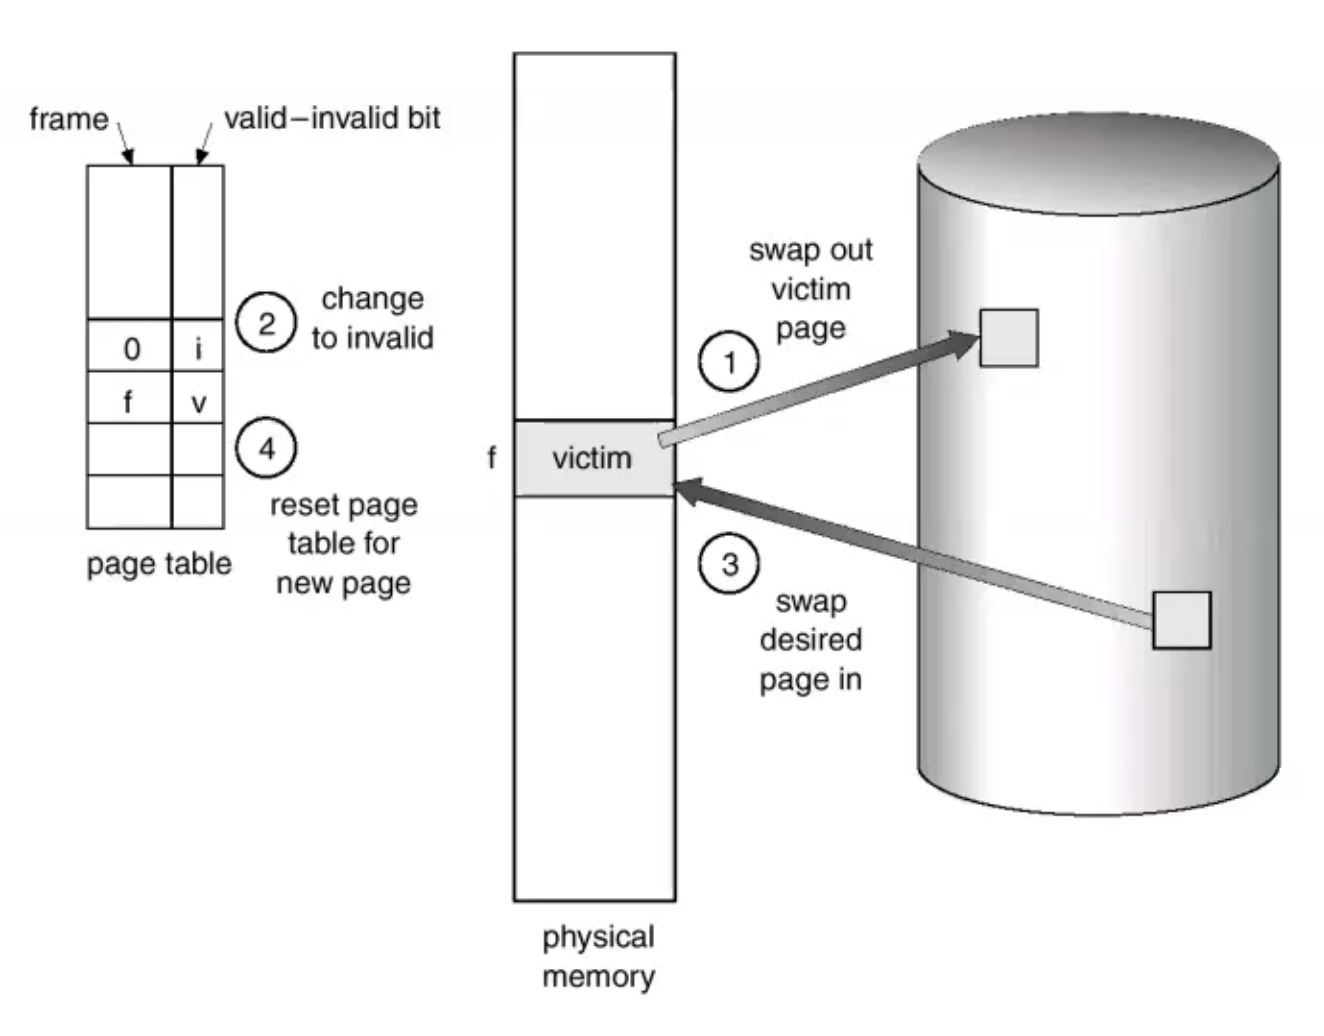
\includegraphics[scale=0.25]{replacement_scheme}
\end{center}


\subsubsection{Prestazioni}
In assenza di frame liberi, sono necessari due accessi alla memoria. Uno per lo \emph{swap out} della 
"vittima" e uno per lo \emph{swap in} del frame da caricare. In questo modo si ha un tempo di page fault 
raddoppiato. 
L'ottimizzazione prevede di inserire nella page table un bit di modifica (\texttt{dirty bit}). Viene messo
a 1 se la pagina \`e stata modificata dal momento in cui \`e stata caricata in memoria. Solo le pagine 
modificate devono essere effettivamente scritte su disco quando diventano "vittime". 

\subsubsection{Problematiche}
Le problematiche principali da analizzare con questa tecnica sono due: quale pagina conviene rimpiazzare, 
e quanti frame assegnare ad un processo al momento dell'esecuzione?

\section{Algoritmi di rimpiazzamento delle pagine}

L'obbiettivo \`e quello di minimizzare il tasso di page fault. La valutazione avviene attraverso un 
meccanismo di riferimenti astratti (\emph{reference string}). Quando la CPU genera un riferimento alla 
RAM, significa che genera un idnirizzo, che poi verr\`a tradotto in un indirizzo fisico attraverso la 
tabella delle pagine. Se si verifica un page fault, dipende dalla porzione di indirizzo che si riferisce 
alla pagina; infatti, una volta caricata una pagina, tutti gli offset al suo interno non potranno causare
page fault (eccezion fatta se la pagina subisce un \emph{swap out}). Perci\`o tutti gli accessi 
consecutivi alla \underline{stessa pagina} causano al massimo un page fault. 

Assumendo di avere gli indirizzi: 100, 604, 128, 130, 256, 260, 264, 268 e avendo pagine della dimensione 
di 100byte, la \emph{reference string} sar\`a 1, 6, 1, 1, 2, 2, 2, 2. Che possiamo ridurre a 1, 6, 1, 2.


Generalmente, il numero di page fault che posso ottenere \`e \emph{inversamente proporzionale} al numero 
di frame.

\begin{center}
    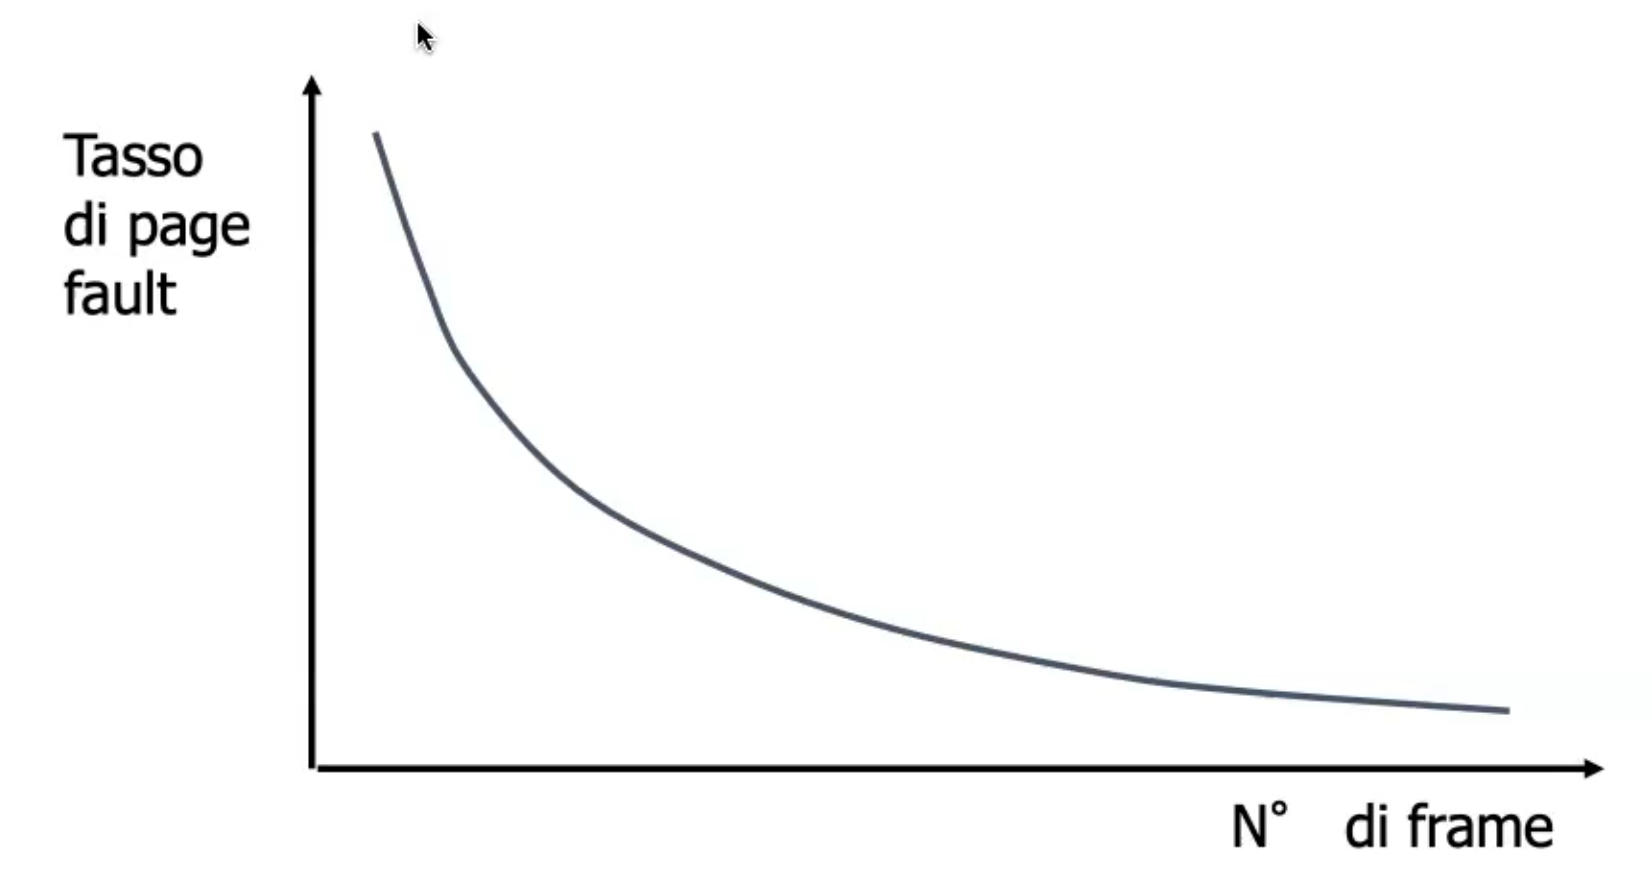
\includegraphics[scale=0.135]{page_vs_frame}
\end{center} 

\subsection{Algoritmo FIFO}
Con questa strategia, la prima pagina introdotta \`e la prima ad essere rimossa. \`E un algoritmo "cieco",
che non valuta l'importanza della pagina rimossa, dove l'importanza \`e data dalla frequenza di riferimento.
Questo algoritmo tende ad aumentare il tasso di page fault. Inoltre, soffre dell'\textbf{anomalia di Belady},
ovvero a volte concedere pi\`u frame porta ad avere pi\`u page fault. 

\subsubsection{Esempio}

Consideriamo una memoria con 3 frame, in un contesto di paginazione su domanda. Con l'algoritmo FIFO otteniamo 15 page 
fault. 
\begin{center}
    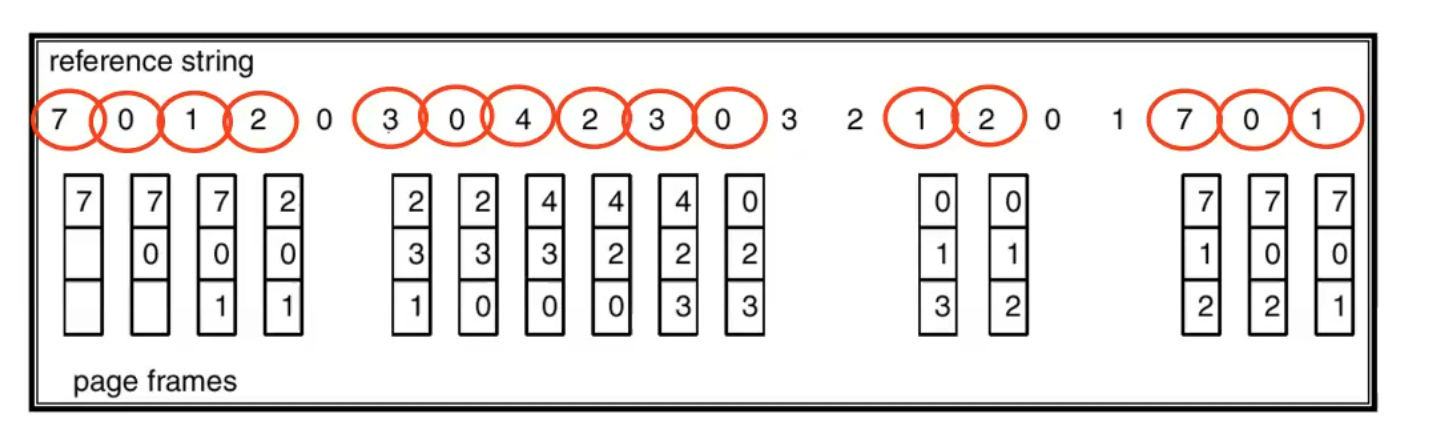
\includegraphics[scale=0.2]{page_faultFIFO}
\end{center} 

\subsubsection{Anomalia di Belady}
Con questo esempio si pu\`o notare che all'aumento dei frame aumentano i page fault. 
\begin{center}
    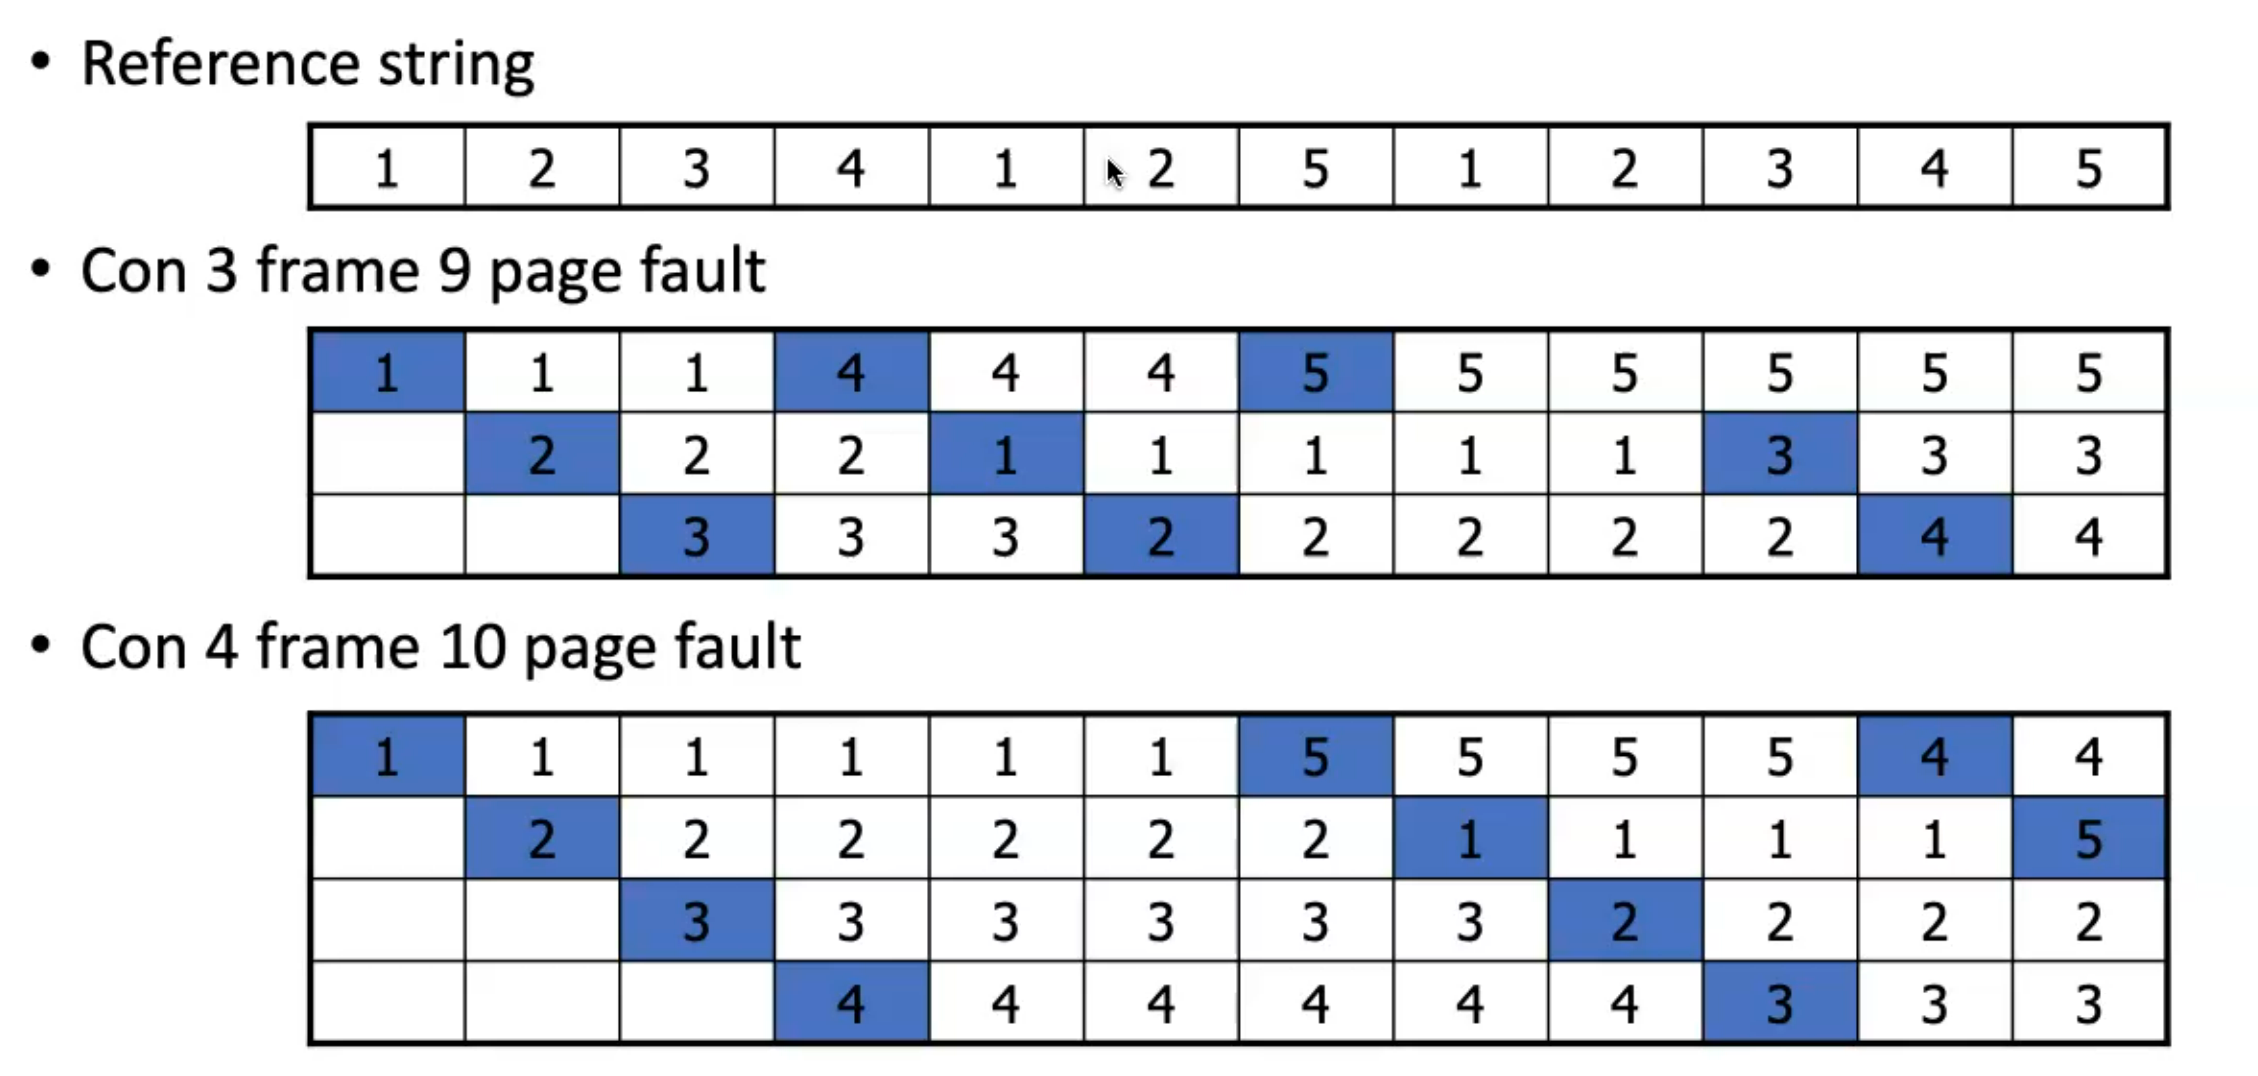
\includegraphics[scale=0.15]{belady_example}
\end{center} 

In conclusione possiamo dire che la tecnica FIFO non \`e una buona strategia perch\'e, oltre all'anomalia di Belady, non considera l'importanza della 
pagina che elimina. 

\subsection{Algoritmo ideale}

L'algoritmo ideale deve garantire il minimo numero di page fault. L'idea \`e quella di rimpiazzare le pagine che non 
verranno usate per il periodo di tempo pi\`u lungo. Il problema risiede nel ricavare questa informazione: richiede una 
conoscenza anticipata della stringa dei riferimenti. Inoltre, l'implementazione di questo algoritmo \`e complessa e 
richiede un supporto hardware dedicato. 
Questo algoritmo rimane comunque un'utile base di partenza per altri algoritmi con le dovute approssimazioni. 

\subsubsection{Esempio} 
Nello stesso contesto precedente, l'algoritmo ideale genera 9 page fault. 
\begin{center}
    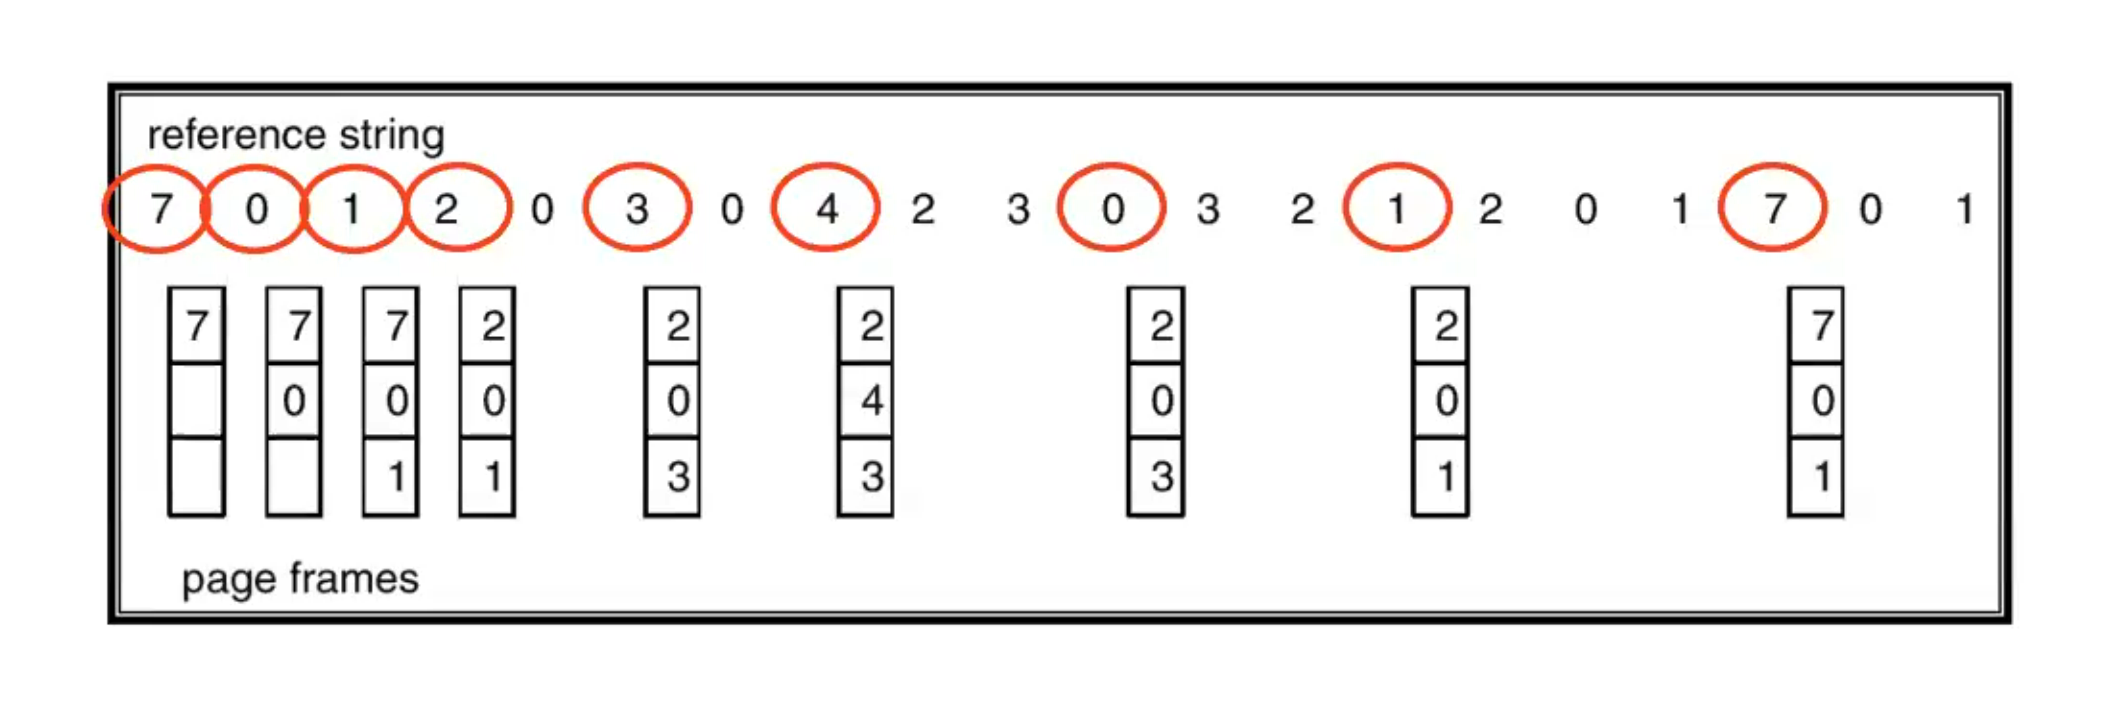
\includegraphics[scale=0.15]{ideal_alg}
\end{center} 

\subsection{Algoritmo LRU}

L'algoritmo ideale non \`e applicabile, ma la migliore approssimazione \`e data dall'algoritmo LRU, \emph{Least Recently
Used}. L'idea di questo algoritmo \`e di utilizzare il passato recente come previsione del futuro, si rimpiazza la pagina 
che non viene usata da pi\`u tempo. 

\subsubsection{Esempio}
L'algoritmo LRU genera 12 page fault, peggiore dell'algoritmo ideale, ma migliore di FIFO.  
\begin{center}
    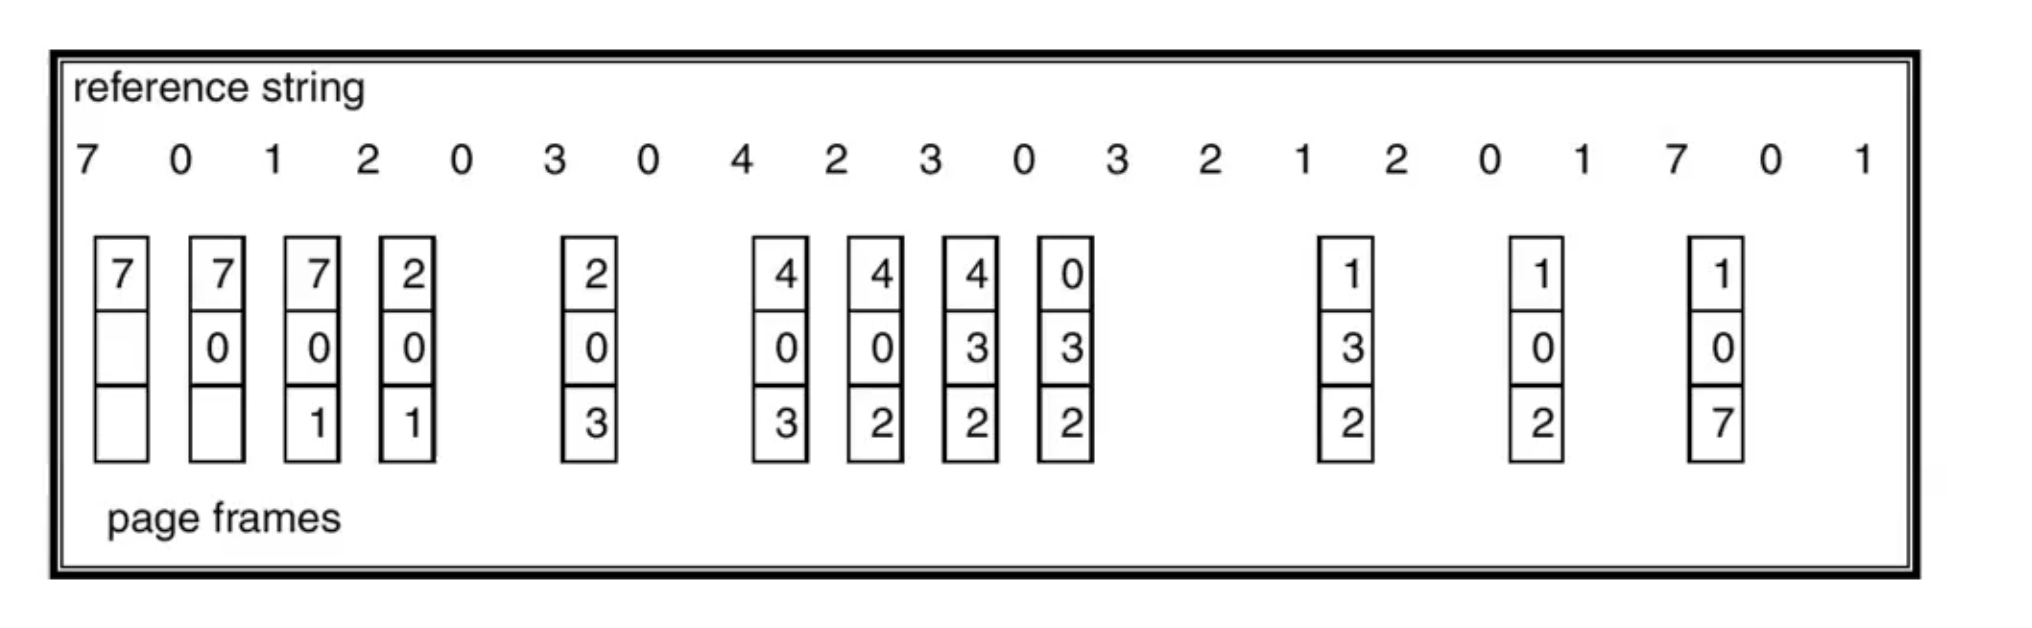
\includegraphics[scale=0.15]{lru_alg}
\end{center}

\subsubsection{Implementazione di LRU}
Non \`e banale ricavare il tempo dell'ultimo utilizzo, potrebbe richiedere un'aggiunta notevole di hardware. 
Le possibili soluzioni implementative sono: 
\begin{itemize}
    \item \textbf{Orologio}: salvare un timestamp dell'ultimo riferimento alla pagina, aggiungerebbe ulteriori bit alla 
        page table e necessit\`a di una ricerca tra i vari timestamp per decidere quale pagina eliminare. 
    \item \textbf{Contatore}: riduce la complessit\`a rispetto al salvataggio del clock, ma diventa necessaria una 
        ricerca fra le pagine di quella col contatore minore. 
    \item \textbf{Stack}: mantenendo uno stack dei numeri di pagina, ad ogni riferimento ad una pagina, questa viene 
        riportata in cima allo stack. \`E necessario aggiornare lo stack rimuovendo un elemento interno allo stack, quindi 
        \`e necessario dell'hardware addizionale. In questo caso il fondo dello stack corrisponde alla pagina "vittima", 
        non \`e necessario fare una ricerca della pagina da rimpiazzare. 
\end{itemize}
Tutte queste tecniche presentano problematiche non banali. La soluzione \`e un'approssimazione dell'algoritmo LRU. 
Usando un \emph{reference bit} associato ad ogni pagina, inizializzato a 0, e messo a 1 dall'hardware quando la pagina 
viene referenziata. Il rimpiazzamento sceglie una pagina che ha il bit a 0. Non viene verificato l'ordine di riferimento 
delle pagine. In alternativa si pu\`o utilizzare un \emph{registro di scorrimento}, ovvero pi\`u bit di reference per ogni 
pagina. I bit vengono aggiornati periodicamente (per esempio ogni 100ms). A questo punto l'algoritmo LRU sceglie la pagina 
vittima quella con il valore pi\`u basso del registro di scorrimento, considerandolo come un intero. 

\subsection{Algoritmo dell'orologio (\emph{second chance})}

Supponendo di avere un orologio esteso che contiene le varie pagine. A ciascuna pagina \`e associato un bit di riferimento. 
L'orologio possiede due lancette, con un angolo $\alpha$ tra loro fissato a priori. 
Ogni spostamento sar\`a una nuova finestra remporale. 

La prima lancetta, al raggiungimento di una pagina, imposta il bit di riferimento a 0, candidandola per l'eliminazione. 
Nel frattempo che cambiano le localit\`a spazio temporali di riferimento (le lancette si sono spostate), se la pagina \`e 
stata riferita nuovamente, il sistema operativo imposta a 1 il bit di riferimento. 

La seconda lancetta \`e quella che decide la pagina \emph{vittima} al momento del verificarsi di un page fault. Se la 
pagina puntata dalla seconda lancetta ha il bit di riferimento uguale a 0, la pagina \`e selezionata come vittima. Se la 
pagina puntata ha invece il bit di riferimento a 1, la seconda lancetta prosegue fino alla prima, cercando la prima 
pagina con il bit di riferimento a 0 all'interno dell'intervallo.
\begin{center}
    \begin{tikzpicture}
        \coordinate (a) at (0,1);
        \coordinate (b) at (0.84, 0.54);
        \coordinate (c) at (0, 0);
        
        
        % Orologio 
        \filldraw[color=black, fill=white] (0,0) circle(4);
        \filldraw[color=black, fill=black] (0,0) circle(0.1);

        % Lancette 
        \draw[->] (0,0) -- (0,2.75);
        \draw[->] (0,0) -- (2.3,1.5);
        
        % Reference bit
        \draw (-0.25, 3) rectangle ++(0.5, 0.5);
        \draw (2.56, 1.56) rectangle ++(0.5, 0.5);

        \draw pic[draw,fill=white,angle radius=1cm,"$\alpha$" shift={(2.5mm,10mm)}] {angle=b--c--a};
    \end{tikzpicture} 
\end{center} 

\subsection{Approssimazioni basate sul conteggio}

Ci sono delle tecniche di approssimazione dell'algoritmo LRU che si basano sul conteggio, ovvero quante volte la 
pagina \`e stata riferita. Queste tecniche si dividono in due tipi, \emph{LFU (Least Frequently Used)}, e \emph{MFU (Most Frequently Used)}.

\subsubsection{Algoritmo LFU}

\begin{itemize}
\item Conteggia il numero di riferimenti fatti a ogni pagina;
\item Rimpiazza la pagina con il conteggio pi\`u basso;
\end{itemize}
Pu\`o non corrispondere alla pagina scelta con LRU, ad esempio se si hanno molti riferimenti iniziali, una pagina
pu\`o avere un alto conteggio e non essere eseguita da molto tempo. 


\subsubsection{Algoritmo MFU}

\begin{itemize}
\item Conteggia il numero di riferimenti fatti ad ogni pagina;
\item Rimpiazza la pagina con il conteggio pi`\u alto;
\end{itemize}
La pagina con il conteggio pi\`u basso \`e probabilmente appena stata caricata e dovr\`a essere persumibilmente
usata ancora, potrebbe essere appena entrata nella localit\`a spazio-temporale del processo!

\subsection{Allocazione dei frame}

Oltre alle tecniche di rimpiazzamento delle pagine, c'\`e un altro aspetto che pu\`o impattare pesantemente sulla CPU
quando accede alla memoria, e dipende da quanto spazio viene concesso ai processi. 
Quindi, data una memoria con $N$ frame e $M$ processi, quanti frame devono essere allocati per ogni processo?

I vincoli da tenere a mente sono che, ogni processo necessita di un minimo numero di pagine per essere eseguito e 
l'istruzione interrotta da un page fault dev'essere fatta ripartire. 

Di conseguenza, il minimo numero di pagine \`e uguale al massimo numero di indirizzi 
specificabili in una \emph{istruzione} (assembly). I valori tipici sono 2-4 frame. 

\subsubsection{Esempio}
Nell'IBM 370 un'istruzione \emph{move} occupa 6 bytes e pu\`o coinvolgere due pagine. 
Di conseguenza servono:
\begin{itemize}
    \item 2 pagine per gestire l'istruzione;
    \item 2 pagine per gestire la sorgente;
    \item 2 pagine per gestire la destinazione
\end{itemize}
\paragraph{Nota:} Il vincolo si dimezza se l'architettura non permette all'istruzione 
di essere a cavallo di due pagine. 

\defbox{\textbf{Allocazione fissa}: un processo ha sempre lo stesso numero di frame.}
\defbox{\textbf{Allocazione variabile}: il numero di frame allocati a un processo pu\`o variare durante l'esecuzione.}

A seconda del contesto, dove scegliere le vittime quando si deve rimpiazzare una pagina?
Se il rimpiazzamento \`e \emph{locale}, ogni processo seleziona vittime solo fra i suoi frame; mentre, se 
il contesto \`e \emph{globale}, il processo pu\`o scegliere frame dall'insieme di \emph{tutti i frame}, quindi 
anche quelli di un altro processo. Questa soluzione \`e preferibile al rimpiazzamento locale perch\'e migliora 
il \emph{throughput}.

\begin{center}
\begin{tabular}{| c || c | c |}
    \hline
    & Contesto  locale & Contesto  globale \\
    \hline 
    \hline 
    Allocazione  Fissa & X & No \\
    \hline
    Allocazione  Variabile & X & X \\
    \hline 
\end{tabular} 
\end{center}

\subsection{Allocazione fissa}
L'allocazione fissa \`e la pi\`u facile da implementare. Ci sono due modi per farlo:
\defbox{\textbf{Allocazione in parti uguali}: Dati $m$ frame e $n$ processi, alloca a ogni processo 
$\frac{m}{n}$ frame.}
\defbox{\textbf{Allocazione proporzionale}: Alloca in proporzione alla dimensione del processo. Questo pu\`o 
non essere un parametro significativo.}

\`E bene notare che la priorit\`a di un processo pu\`o essere pi\`u significativa della  sua dimensione.

\subsubsection{Esempio}
Dati $s_i$ size del processo $p_i$, $S = \sum s_i$, il numero totale dei frame $m$, si ha che l'allocazione $a_i$
per il processo $p_i$ si calcola come 
\[a_i  = \left( \frac{s_i}{S} \right) m.\]
Considerando $m = 64$, $s_1 = 10$, $s_2 = 127$, abbiamo che 
\[ a_1 = \left(\frac{10}{137} \right)64 \approx 5; \thickspace \thickspace a_2 = \left(\frac{127}{137}\right)64 \approx 59.\]

\subsection{Allocazione variabile}

Permette di modificare dinamicamente le allocazioni ai vari processi. Si deve per\`o trovare una strategia: sulla base di 
cosa modifico l'allocazione? 

Ci sono due soluzioni: 
\begin{enumerate}
    \item Calcolo del \emph{working set}.
    \item Calcolo del \emph{page fault frequency (PFF)}.
\end{enumerate}

\subsubsection{Working set}

\`E un'approssimazione della localit\`a del programma. Il criterio per rimodulare l'allocazione 
dei frame in base alle richieste effettive di ogni processo. Questa tecnica sfrutta il concetto 
della localit\`a spazio temporale. 

Un processo, dunque, necessit\`a di un numero di frame pari alla sua localit\`a spazio temporale. 
Per misurare quest'ultima si deve fare una stima rispetto al comportamento dei processi nel passato 
recente. 

\begin{center}
    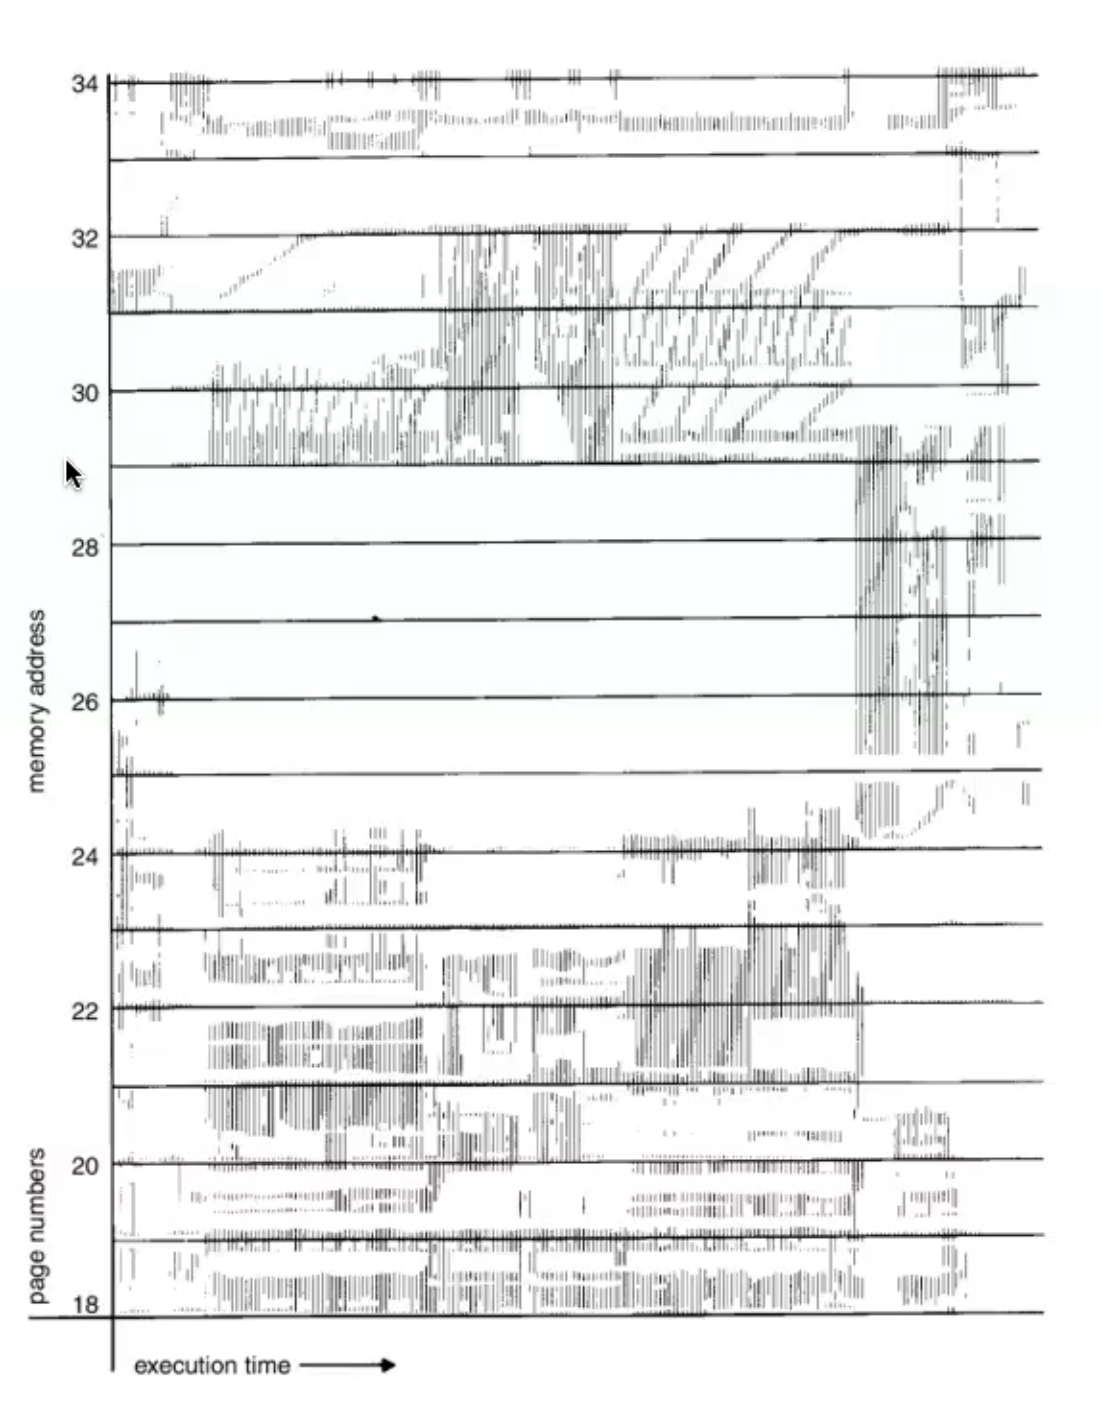
\includegraphics[scale=0.2]{working_set}

    \tiny{Grafico della localit\`a d'esecuzione.}
\end{center}

\subsubsection{Calcolo del working set}

Consideriamo che il processo $P_i$ riceva frame sufficienti a mantenere in memoria il suo \emph{working set} $WS_i (t, \Delta)$.
$\Delta$ \`e la finestra temporale del working set; si deve verificare il numero di pagine referenziate nell'intervallo di 
tempo $[t-\Delta, t]$ pi\`u recente. Notare che se $\Delta$ \`e piccolo, la previsione ricavata sar\`a poco precisa, mentre se 
$\Delta$ \`e troppo grande, potrebbe coprire pi\`u d'una localit\`a, ($\Delta = \infty \Rightarrow$ \emph{tutto il programma}).

\begin{center}
    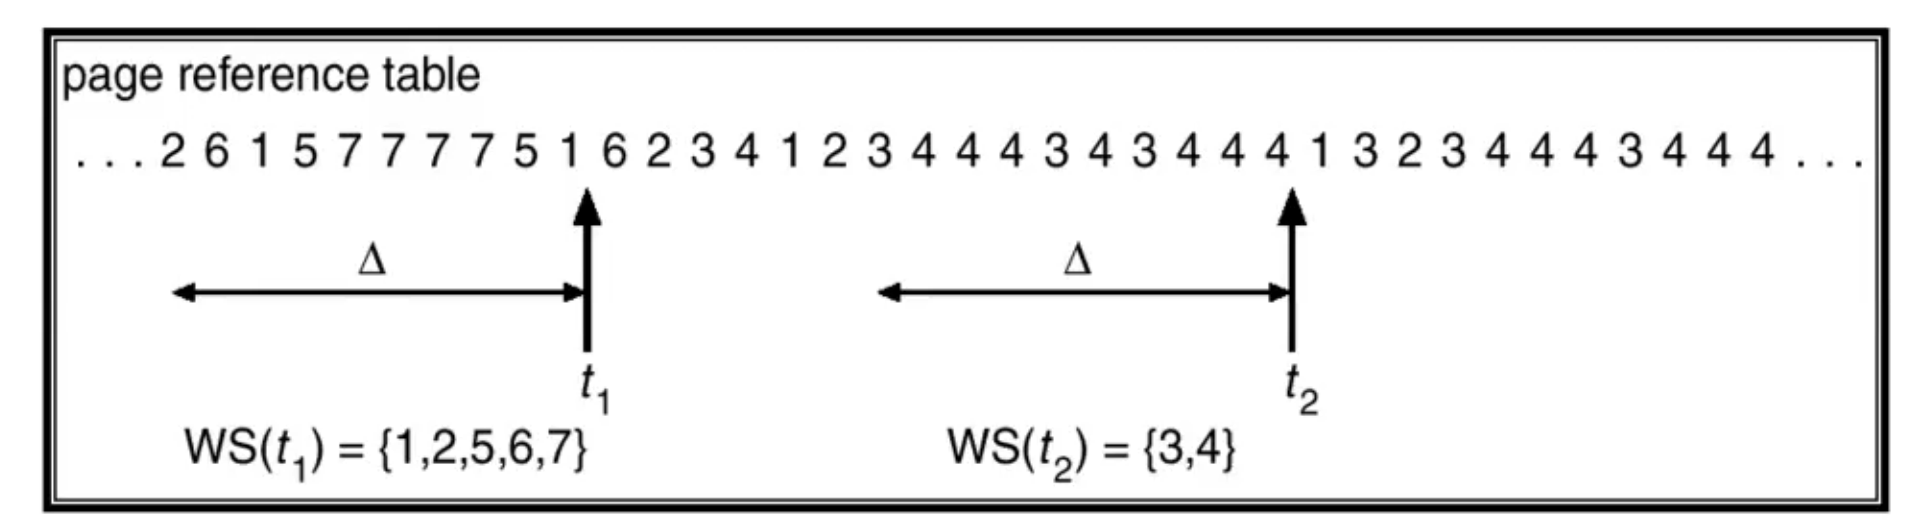
\includegraphics[scale=0.2]{working_set_example}
\end{center}

\subsection{Trashing}
Cosa succede se i frame sono pochi?
\[ D = \sum_i WSS_i = richiesta\thickspace totale \thickspace di \thickspace frame\]
Se $D$ \`e maggiore del numero totale dei frame, si verifica il fenomeno del \emph{trashing}, ovvero un blocco 
del sistema occupato a swappare pagine da e verso la memoria. Di conseguenza la \emph{ready queue} si svuota e 
si abbassa l'utilizzo della CPU, che deve gestire i page fault. A questo punto il sistema operativo tende ad 
aumentare il grado di multiprogrammazione aggiungendo processi, che aumentano il tasso di page fault. Questo 
circolo vizioso fa si che, ad un certo punto, il \emph{throughput} precipita. 

Per questo motivo \`e necessario stimare con esattezza il numero di frame necessari a un processo per non 
entrare in trashing. 

\begin{center}
    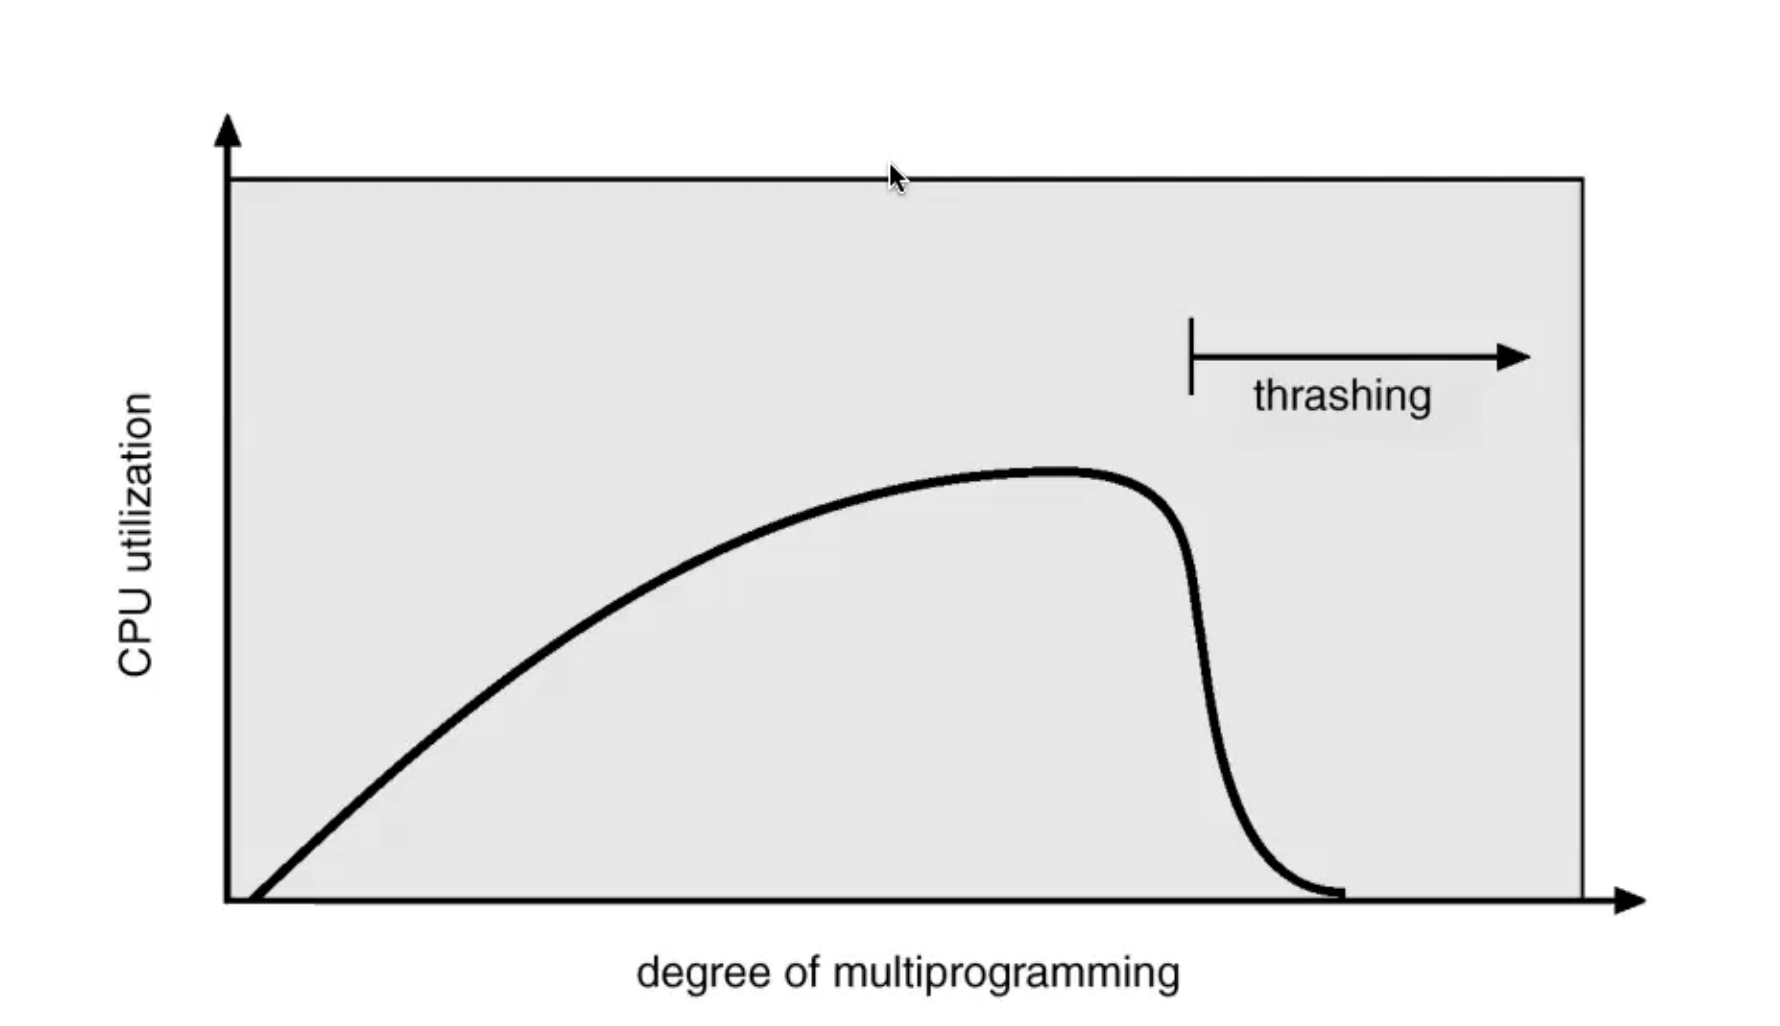
\includegraphics[scale=0.2]{trashing_diagram}
\end{center}

Il metodo corretto per misurare il working set \`e attraverso un'approsimazione tramite timer e \emph{bit di 
reference}. Il timer interrompe periodicamente la CPU, all'inizio di ogni periodo, i bit di reference sono posti a 0 e, 
ad ogni interruzione del timer, le pagine vengono scandite. Quelle con il bit di reference uguale a 1, sono nel working set, 
mentre quelle con il bit di reference uguale a 0 vengono scartate. In questo caso per\`o viene scartato (messo nella swap area), 
l'intero processo a cui la pagina appartiene. In questo modo non si pu\`o innsecare il circolo vizioso descritto in precedenza. 

L'accuratezza della previsione aumenta sulla base del numero di bit di reference e sulla frequenza delle interruzioni. 

\subsubsection{Page fault frequency}

Un'alternativa pi\`u semplice e pi\`u accurata del calcolo del working set \`e quella 
del calcolo del PFF. La strategia prevede di stabilire un tasso di page fault accettabile e mantenerlo attraverso 
la concessione o il rilascio di frame ai processi. 

Perci\`o se il tasso effettivo di page fault \`e troppo 
basso per un processo, ovvero sta sotto al \emph{lower bound}, deve rilasciare frame, perch\'e ne 
ha troppi; se il tasso \`e troppo alto, quindi supera l'\emph{upper bound}, il processo ottiene pi\`u frame. 

\begin{center}
    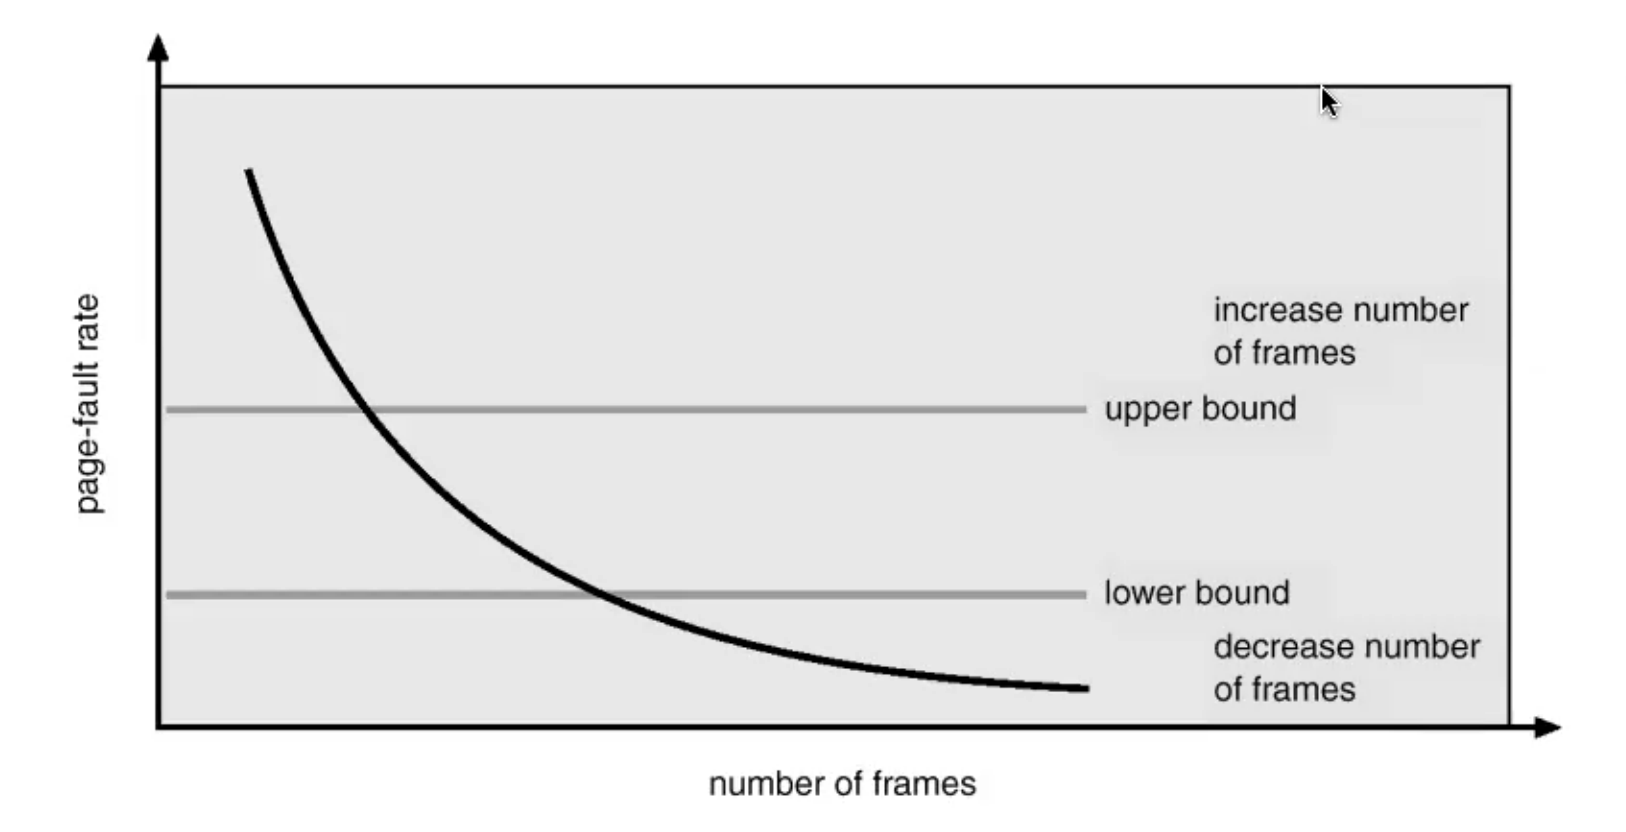
\includegraphics[scale=0.2]{pff_graph}
\end{center}

\subsubsection{Considerazioni: dimensione pagina (= frame)}

\begin{enumerate}
    \item \textbf{Frammentazione}: pagine \emph{grandi} portano ad una maggiore frammentazione interna. 
    \item \textbf{Localit\`a}: pagine \emph{grandi} portano al trasferire in memoria anche ci\`o che 
    non \`e necessario, perc\'e fuori dalla localit\`a. 
    \item \textbf{Dimensione page table}: pagine \emph{piccole} comportano l'avere molte entry nella tabella.
    \item \textbf{I/O overhead}: pagine \emph{piccole} aumentano il costo di lettura/scrittura.
\end{enumerate}

I punti $1$ e $2$ ci fanno preferire l'implementazione di pagine \emph{piccole}, mentre i punti $3$ e $4$ ci 
fanno preferire pagine \emph{grandi}.

\subsubsection{Considerazioni: struttura dei programmi}

La struttura di un programma influisce sul numero di page fault che possono essere generati. 
Se consideriamo un programma che deve inizializzare un array di interi \texttt{A[1024,1024]}, con una 
riga memorizzata in una pagina e un solo frame assegnato al processo. Consideriamo i le seguenti
implementazioni:

\begin{lstlisting}
    for j := 1 to 1024 do 
        for i := 1 to 1024 do 
            A[i,j] := 0;
\end{lstlisting}
Vengono generati \textbf{1024 $\times$ 1024} page fault.

\begin{lstlisting}
    for i := 1 to 1024 do 
        for j := 1 to 1024 do 
            A[i,j] := 0;
\end{lstlisting}
Vengono generati \textbf{1024} page fault. 

Questo avviene perch\'e, nella prima implementazione lo scorrimento avviene per riga, 
quindi deve ricaricare la pagina con il primo elemento della prima riga, inizializzarlo 
e poi ricaricare la pagina con il primo elemento della seconda riga, eccetera.

Nel secondo caso, l'implementazione prevede uno scorrimento per colonna, quindi una volta 
caricata nella pagina la prima riga, inizializzo tutte le colonne e il page fault avverr\`a 
solo al caricamento delle righe. 

% Lezioni di riferimento 04/05/2023
% Libro di rif. Silberschatz - Galvin pag. 485 e seguenti, capitolo 11.
\chapter{Memoria secondaria}

\section{Tipologia di supporto}

Il principale sistema di archivazione di massa nei computer moderni \`e la memoria secondaria, che di
solito \`e fornita da dischi rigidi o altri dispositivi di memoria non volatile, come nastri magnetici, 
dischi magnetici (HDD) e dispositivi a stato solido (SSD).

\subsection{Nastri magnetici}

Sono una sottile striscia di materiale plastico, rivestita di un materiale magnetizzabile. Usati per 
memorizzare dati digitali per la prima volta nel 1951 sul Eckert-Mauchly UNIVAC I.

La massima capienza raggiunta \`e di 5TB nel 2011. Il principale problema di questo tipo di supporto 
\`e l'accesso sequenziale, che per riposizionare la testina di lettura richiede diversi secondi. Sono
circa 3 ordini di grandezza pi\`u lenti dei dischi magnetici.

\subsection{Dischi magnetici}

Si tratta di piatti d'alluminio (o di altro materiale) ricoperti di materiale ferromagnetico, al 2017 la
capienza massima era di 10TB. La riduzione del diametro dei dischi ha permesso di aumentarne la velocit\`a
di rotazione. Il diametro varia da $3.5$ pollici per i sistemi desktop fino a $1$ pollice per i dispositivi
mobili. 

La principale caratteristicha dei dischi magnetici \`e l'accessibilit\`a randomicamente. In scrittura, il passaggio
di corrente positiva o negativa attraverso la testina magnetizza la superficie; mentre in lettura, il passaggio
sopra un'area magnetizzata induce una corrente positiva o negativa nella testina. 

\subsubsection{Struttura}
\begin{center}
    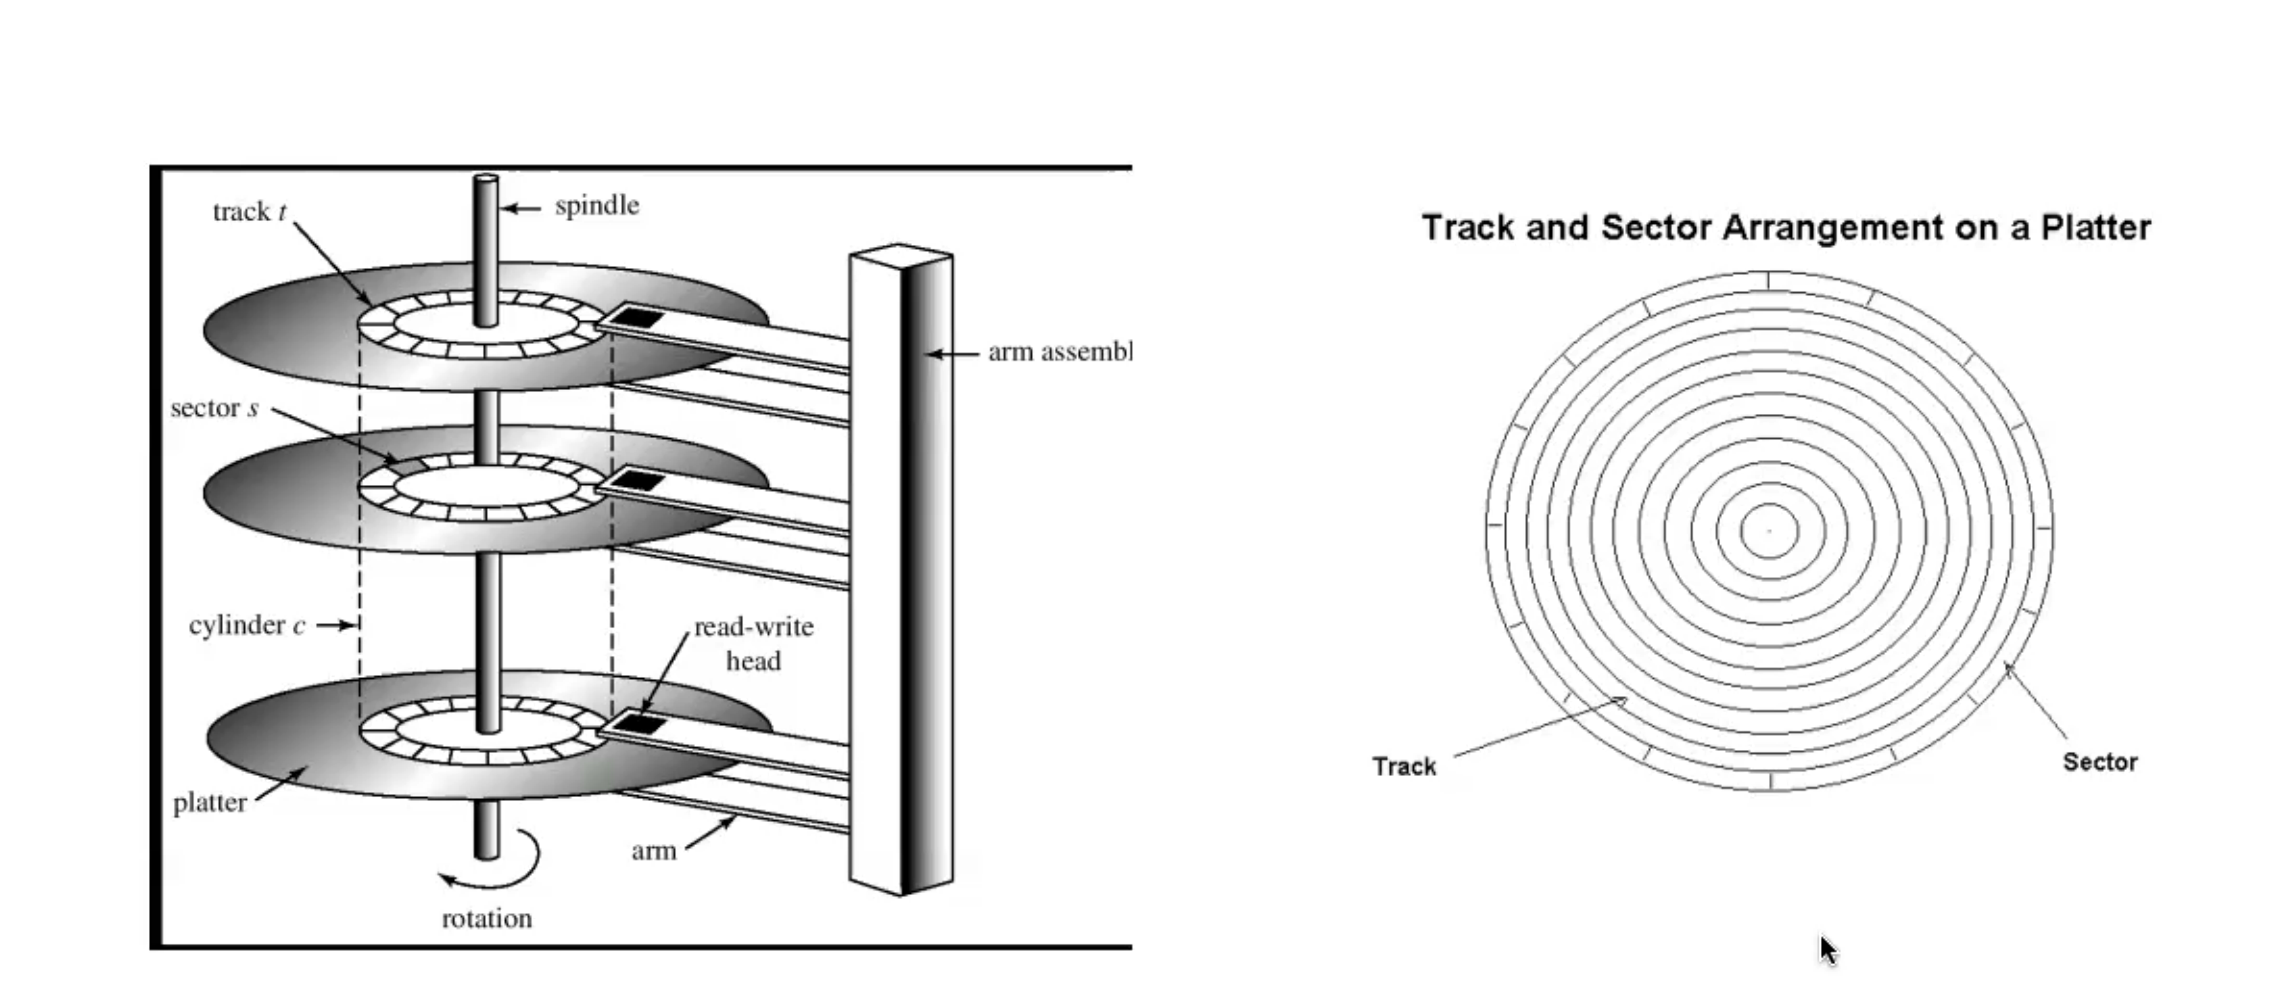
\includegraphics[scale=0.15]{hdd_structure}
\end{center}

\defbox{\textbf{Settore}: \`e l'unit\`a pi\`u piccola di informazione che pu\`o essere scritta/letta su disco.}

La dimensione \`e variabile tra 32 byte e 4KB (solitamente 512 Byte). Generalmente sono raggruppati dal punto 
di vista logico in \emph{cluster} o \emph{blocchi di settori}, per motivi di efficienza. La dimensione dipende
dalla grandezza del disco e dal sistema operativo, da 2KB a 32KB. Questo viene fatto per limitare le operazioni
di scrittura e lettura. Un file occupa sempre almeno un cluster.

Per accedere a un settore bisogna specificare la superficie, la traccia e il settore stesso. 

\subsubsection{Tempo di accesso al disco}

Il tempo di accesso al disco \`e dato da tre componenti,  \emph{seek time, latency} e \emph{transfer time}, secondo 
la formula:
\[ T_{accesso} = T_{seek} + T_{latency} + T_{transfer}.\]
\begin{itemize}
    \item \defbox{\textbf{Seek time}: tempo necessario a spostare la testina sulla traccia.}
    \item \defbox{\textbf{Latency time}: Il tempo necessario a posizionare il settore desiderato sotto la 
    testina, dipende dalla velocit\`a di rotazione.}
    \item \defbox{\textbf{Transfer time}: il tempo necessario al settore per passare sotto la testina, la
    lettura vera e propria.}
\end{itemize}

La componente pi\`u pesante \`e la prima componente \emph{seek time}, che sar\`a quella su cui ci si 
concentrer\`a maggiormente, anche lato software, per migliorare l'efficienza. 
Per quanto riguarda il \emph{latency time}, nel caso pessimo si dovr\`a fare una rotazione del disco, in 
media la rotazione necessaria \`e di mezzo disco. 

\subsubsection{Tempi di accesso - valori}
Analizziamo i valori delle varie componenti:
\begin{itemize}
    \item Seek time: tipicamente $3ms$ (server driver), fino a $15ms$ (mobile driver). Mediamente $9ms$ per
    un disco su desktop;
    \item La latenza \`e in media mezza rotazione del disco per ogni accesso. Si ha:
    \[Latency = 0.5 * (\frac{60s}{v_{rotazione}rpm} = 0.5 * v_{rotazione}). \]
    Per un disco da 7200rmp si ha:
    \[ 0.5 * (\frac{60s}{7200rpm} = 0.5 * {8.3*10^{-3}} = 4.16ms). \]
    \item $Transfer time = \frac{dim. blocco}{v_{trasf}}$.
    Mantenendo l'esempio di un disco da 7200rpm, si ha:
    \begin{itemize}
        \item \textbf{disk-to-buffer} 1030Mbits/sec.
        \item \textbf{buffer-to-computer} 300MB/sec.
    \end{itemize}
\end{itemize}

\subsubsection{Esempio di accesso a disco}
Data $v_{trasf} = 40MB/s$, $v_{rot} = 10000rpm = 166rps$, $Rot_{media} = \frac{1}{2} traccia$,
$Dim_{blocco} = 512 Byte$, $T_{seek} = 5ms$.
Otteniamo che il tempo d'accesso sar\`a:
\[ T_{accesso} = T_{seek} + \frac{Rot_{media}}{v_{rot}} + \frac{Dim_{blocco}}{v_{trasf}} = \]
\[ = 5ms + \frac{0.5}{166rps} + \frac{0.5KB}{40MB/s} = 8.0000125ms.\]

\subsubsection{Considerazione}
Siccome il \emph{seek time} \`e dominante, e si ha un grande numero di processi nel sistema che 
accedono al disco, un modo per minimizzare il seek time tramite \emph{algoritmi di scheduling} per:
\begin{itemize}
    \item ordinare gli accessi al disco per minimizzare il tempo di accesso totale.  Ridurre il seek time
significa ridurre lo spostamento della testina;
    \item massimizzare la banda, ovvero il numero di byte trasferiti in un dato tempo. Misura la velocit\`a effettiva. 
\end{itemize}

\subsection{Dispositivi a stato solido SSD}

I dischi allo stato solido usano la stessa interfaccia dei dischi fissi (HDD) e quindi possono rimpiazzarli
facilmente. Utilizza chip (DRAM o memorie flash NAND) per memorizzare i dati in modo non volatile. Capacit\`a
fino a 2TB.

Gli SSD rispetto agli HD sono meno soggetti a danni, mancando numerosi parti mobili. Di conseguenza sono 
anche pi\`u silenziosi. Sono pi\`u effecienti, l'accesso in ogni parte del disco avviene in tempo costante e
non necessitano di essere defframentate. Di contro, le memorie flash hanno un limite sul numero di write (1-5 milioni).

\section{Scheduling di accesso al disco}

\subsection{Struttura di un disco}
La vista logica di un disco \`e un \emph{vettore unidimensionale} di blocchi logici. Il blocco, o \emph{cluster}, 
\`e la minima unit\`a di trasferimento. 

Il vettore \`e mappato sequenzialmente sui settori del disco: il settore 0 \`e il primo settore della prima traccia
del cilindro pi\`u esterno, mentre l'ultimo settore sar\`a l'n-esimo settore della traccia pi\`u interna. 
La numerazione procede gerarchicamente per settori, tracce e cilindri:
\begin{center}
    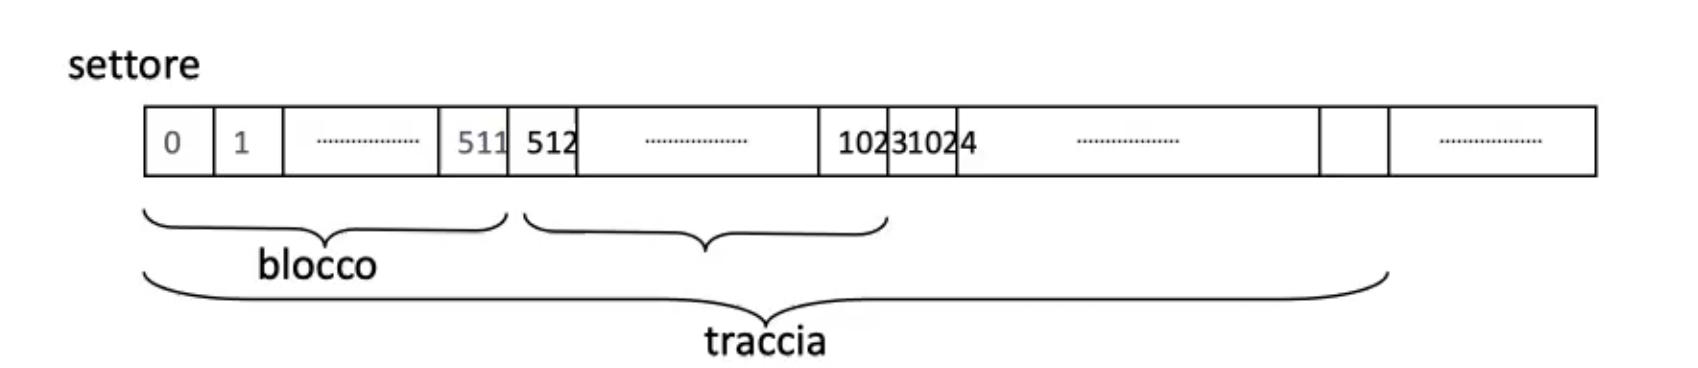
\includegraphics[scale=0.2]{disk_logic}
\end{center}
Il processo che necessita di I/O esegue una system call e il sistema operativo usa la vista logica del disco. La
sequenza di accessi \`e data da una sequenza di indici del vettore.
\begin{center}
    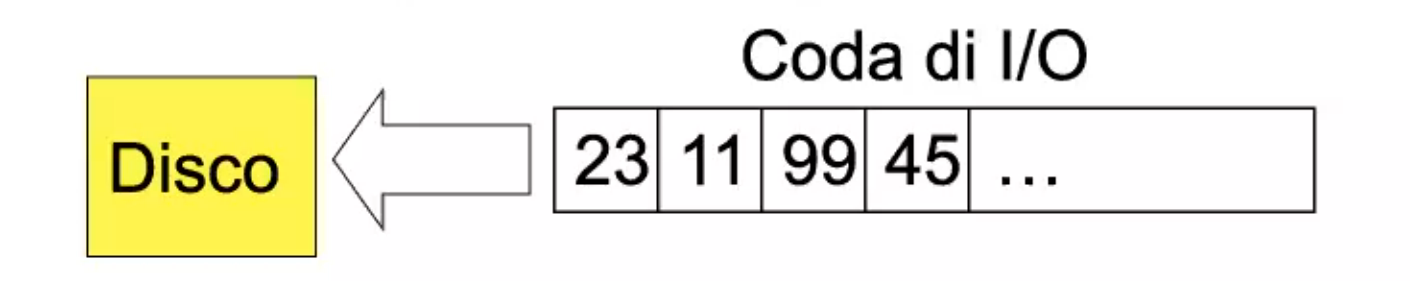
\includegraphics[scale=0.15]{io_queue}
\end{center}
Oltre al numero di blocco, ovvero l'indirizzo di destinazione, nella richiesta di I/O ci saranno le informazioni sul tipo 
di accesso (\emph{read/write}) e la quantit\`a di dati da trasferire. 

\subsection{Algoritmi di disk scheduling}

\`E necessario un compromesso costo/efficacia, come di consueto.

Per analizzare gli algoritmi di disk scheduling, consideriamo di avere la testina sulla traccia 53, e di 
avere la seguente coda di accessi: \texttt{98, 183, 37, 122, 14, 124, 65, 67}. L'intervallo dei valori 
ammissbili $= [0, 199]$.

\subsubsection{FCFS}
Il primo, e il pi\`u semplice algoritmo \`e la coda FIFO. Si processano le richieste nell'ordine d'arrivo.
Possiamo calcolare uno spostamento totale della testina di 640 tracce. 
\begin{center}
    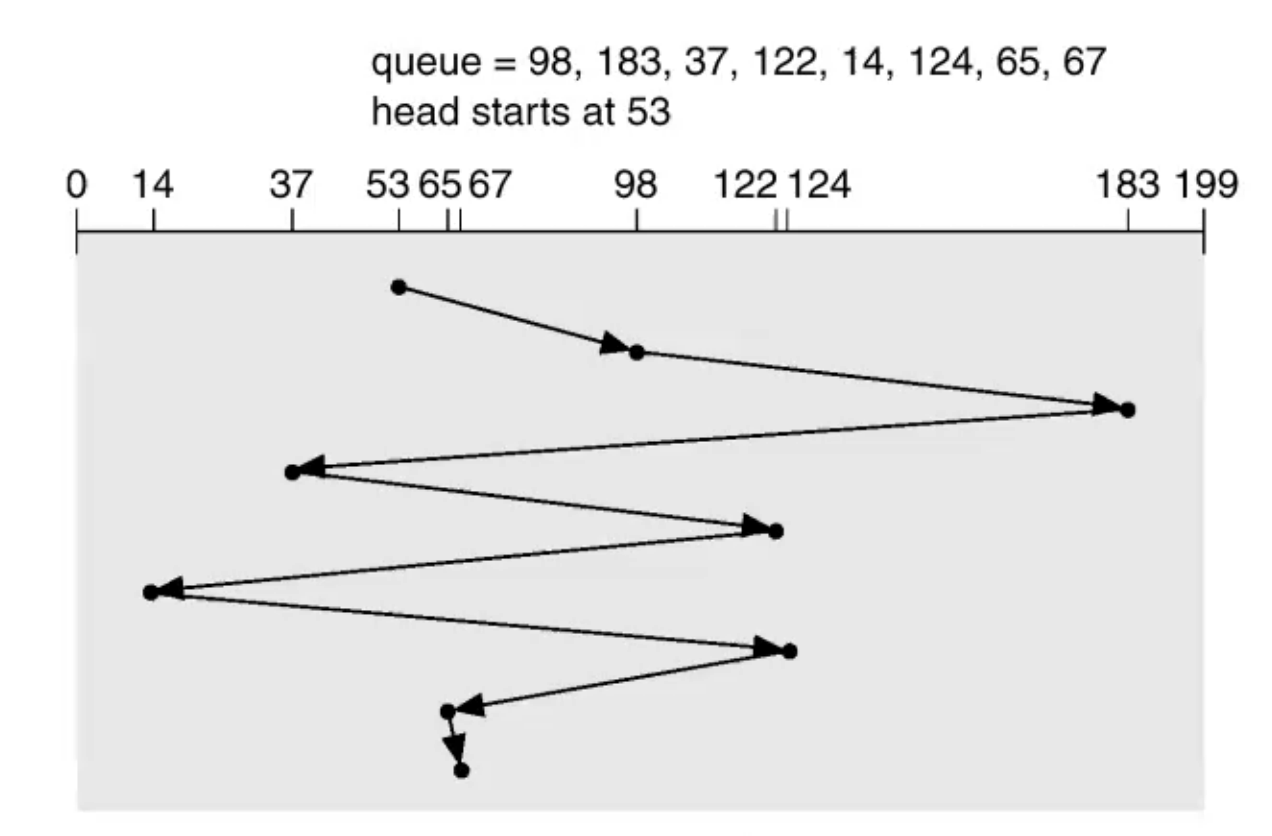
\includegraphics[scale=0.2]{fcfs_disk}
\end{center}

\subsubsection{SSTF}
Una tecnica pi\`u efficiente \`e quella di selezionare la richiesta con il minimo spostamento 
rispetto alla posizione attuale della testina. Questa tecnica \`e detta \emph{Shortest Seek Time First}.
Si migliorano le prestazioni rispetto a FCFS, ma non \`e ottimale, inoltre \`e possibile che alcune 
richieste soffrano di \emph{starvation}. Riprendendo l'esempio precedente, ora lo spostamento totale
della testina \`e di 236 tracce. 
\begin{center}
    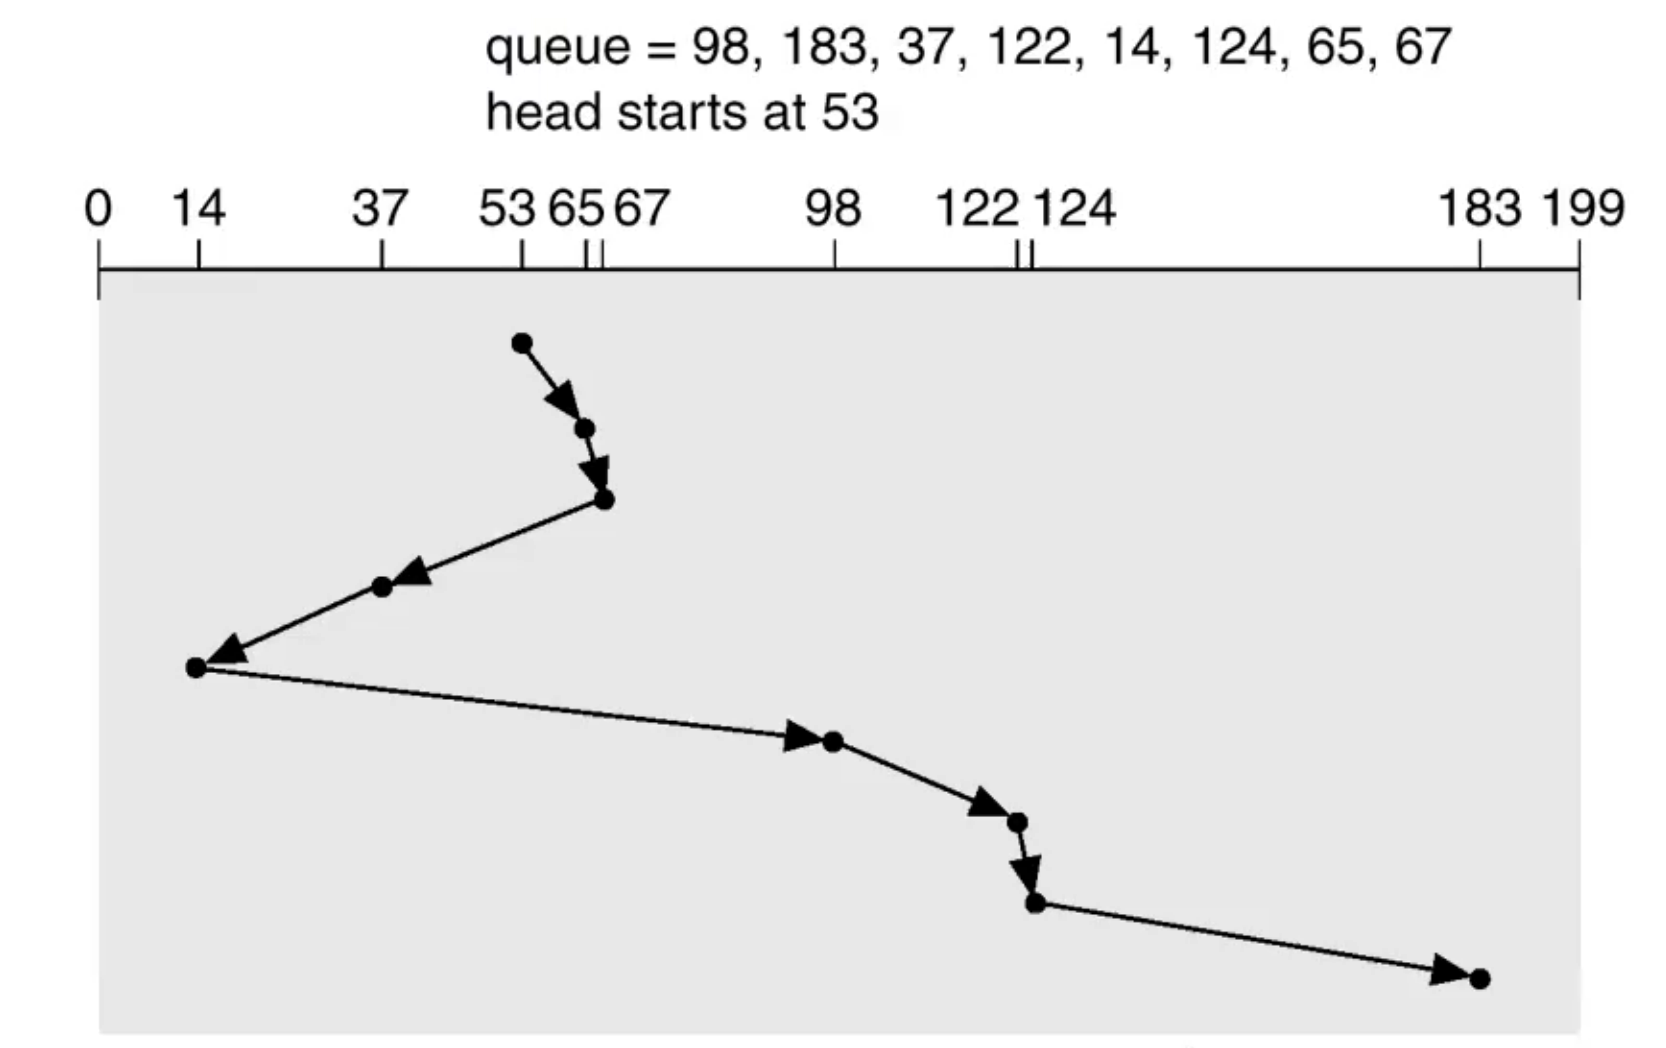
\includegraphics[scale=0.2]{sstf_disk}
\end{center}

\subsubsection{SCAN - Algoritmo dell'ascensore}
La natura dinamica delle richieste porta all'algoritmo SCAN. L'idea \`e che la testina parte da un'estremit\`a
del disco e si sposta verso l'altra estremit\`a, servendo tutte le richieste correnti. Arrivata all'altra 
estremit\`a, riparte nella direzione opposta, servendo le nuove richieste. 

\begin{center}
    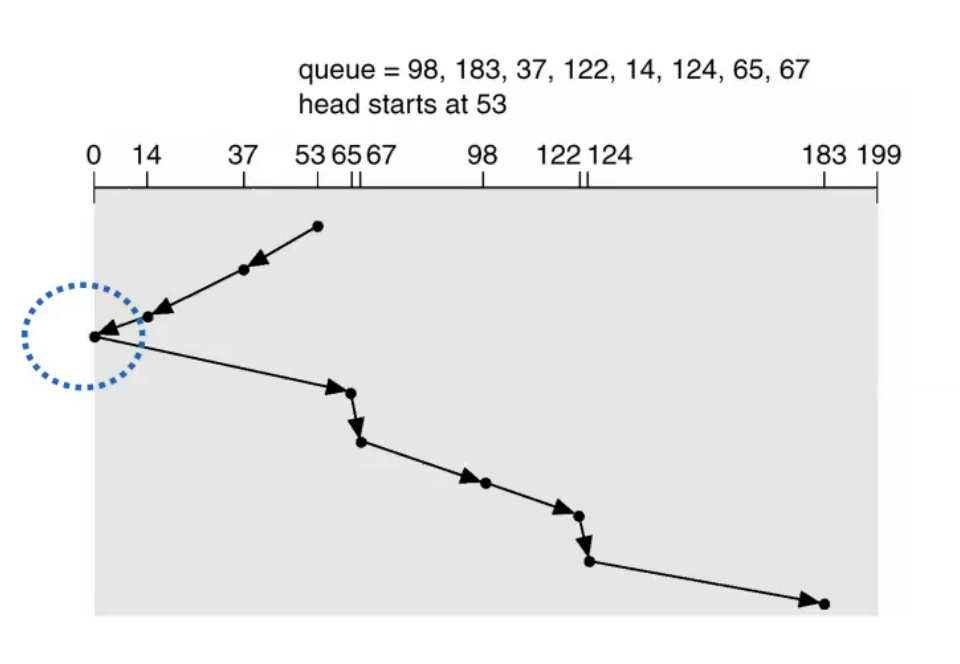
\includegraphics[scale=0.2]{scan_disk}
\end{center}

Lo spostamento totale della testina \`e di 236 tracce. In questo caso non si ha neanche bisogno di riordinare
la coda, perch\'e si segue lo spostamento naturale della testina. 

\subsubsection{CSCAN - Algoritmo dello spalatore di neve}

L'idea alla base \`e l'algoritmo SCAN, ma circolare. Quando la testina arriva ad una estremit\`a riparte
immediatamente da 0 senza servire altre richieste. Il disco viene visto come una lista circolare, il tempo 
d'attesa diventa pi\`u uniforme rispetto a SCAN. Alla fine di una scansione ci saranno pi\`u richieste
all'altro estremo. In questo caso la possibilit\`a di \emph{starvation} \`e mitigata, ma dipende dalla 
densit\`a delle richieste localizzate in un'area pi\`u vicina alla testina rispetto ad altre aree. 
\begin{center}
    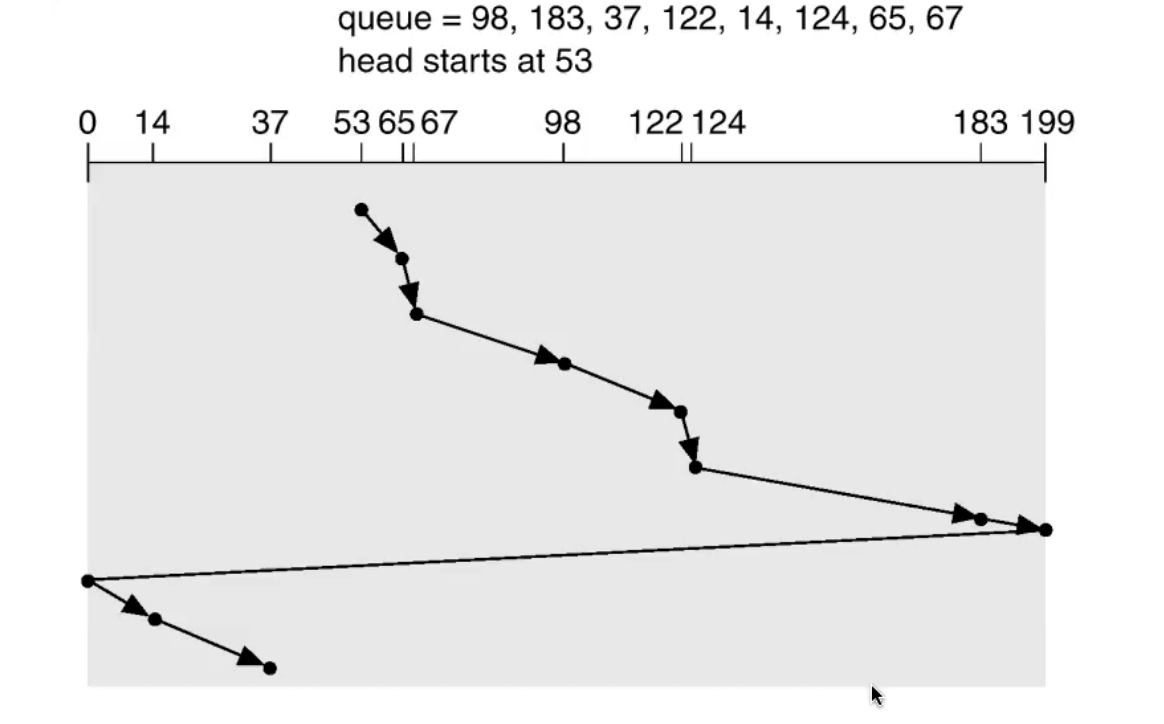
\includegraphics[scale=0.2]{cscan_disk}
\end{center}
Considerando l'esempio, in questo caso lo spostamento totale della testina \`e di 382 tracce.

% Riferimento lezione del 11/05/2023
\subsection{C-LOOK}
In questa variante dello SCAN la testina non arriva sino all'estremit\`a del disco, ma cambia direzione
(LOOK) o riparte dalla prima traccia (C-LOOK) non appena non ci sono pi\`u richieste in quella direzione. 
In questo caso, lo spostamento totale \`e di 322 tracce.
\begin{center}
    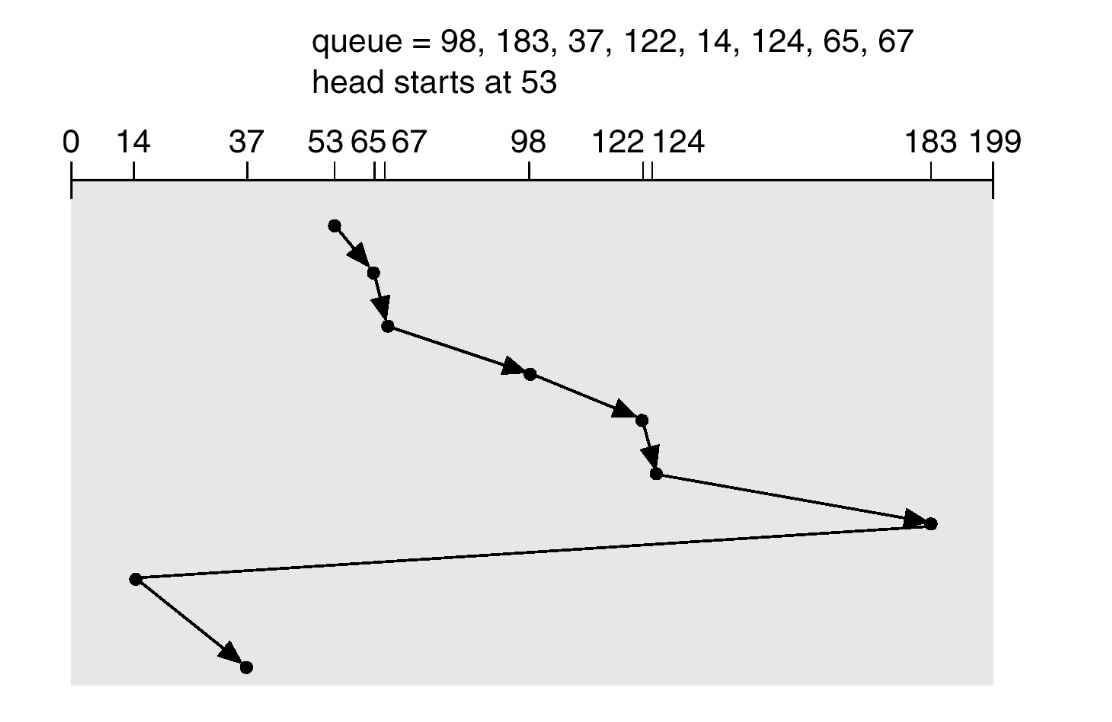
\includegraphics[scale=0.2]{clook_disk}
\end{center}
Anche le varianti LOOK e CLOOK non risolvono totalmente il problema della \emph{starvation}. 

\subsection{N-step SCAN}
In questa variante, per evitare che la testina rimanga sempre nella stessa zona, si divide la coda delle
richieste in pi\`u parti di dimensione massima $N$. Quando una coda viene processata per il servizio 
(scan in una direzione), gli accessi in arrivono riempiono altre code. Dopo che una coda \`e stata riempita
non \`e possibile riordinare le richieste. 

Le code "\emph{sature}" vengono servite nello scan successivo. Questa alternativa, al variare di $N$ ci
avvicina maggiormente allo SCAN puro o all'FCFS. Infatti, per $N$ grande si degenera in SCAN, mentre per
$N = 1$ si tende all'FCFS. 

Un algoritmo simile, ma limitato a solo due code \`e l'FSCAN.

\subsection{LIFO - Last In First Out}

In alcuni casi, pu\`o essere utile schedulare gli accessi in base all'ordine inverso di arrivo. Questa
strategia \`e utile in casi di accessi con elevata localit\`a, ma aumenta la possibilit\`a di \emph{starvation}.

\subsection{Analisi degli algoritmi}

Nessuno degli algoritmi precedenti \`e quello ottimo. L'algoritmo ideale \`e poco efficiente, perch\'e il
risparmio ottenibile non compensa la complessit\`a di calcolo. 

La distribuzione degli accessi, in numero e dimensioni, e l'organizzazione delle informazioni su disco (file system)
sono fattori che influenzano l'analisi. 

Se gli accessi sono molti di dimensioni medio piccole, subiscono in modo relativamente maggiore il 
tempo di \emph{seek}, rispetto a accessi di grandi dimensioni. Inoltre, la distanza dei dati a cui si
vuole accedere rispetto alle estermit\`a del disco incide sul tempo di accesso.

In generale SCAN/C-SCAN sono gli algoritmi migliori per sistemi con molti accessi a disco. Il 
\emph{disk-scheduling} \`e spesso implementato come modulo indipendente dal sistema operativo, con
diverse scelte di algoritmo. 


\section{Gestione del disco}

Quando si vuole usare una memoria di massa, dobbiamo effettuare alcune operazioni che ci permettono di 
utilizzare il supporto fisico per slavare dati.

\subsection{Formattazione dei dischi}

Esistono due tipi di formattazione. La formattazione di basso livello (o \emph{fisica}), consiste nella
divisione del disco in settori che il controllore pu\`o leggere o scrivere. 

Per poter usare un disco come contenitore di file, il sistema operativo deve memorizzare le proprie 
strutture sul disco. Si deve effettuare un partizionamento del disco in uno o pi\`u gruppi di cilindri (partizioni), 
dev'essere eseguita la formattazione \emph{logica}, per creare un file system; infine, dev'esserci un 
programma di boot, per inizializzare il sistema.

Il programma di bootstrap memorizzato nella ROM (bootstrap loader) carica il bootstrap dal disco (dai blocchi
di boot). Inoltre, carica i driver dei dispositivi e lancia l'avvio del sistema operativo. 

\begin{itemize}
    \item Vista concettuale: disco "nudo" 
    \begin{center}
        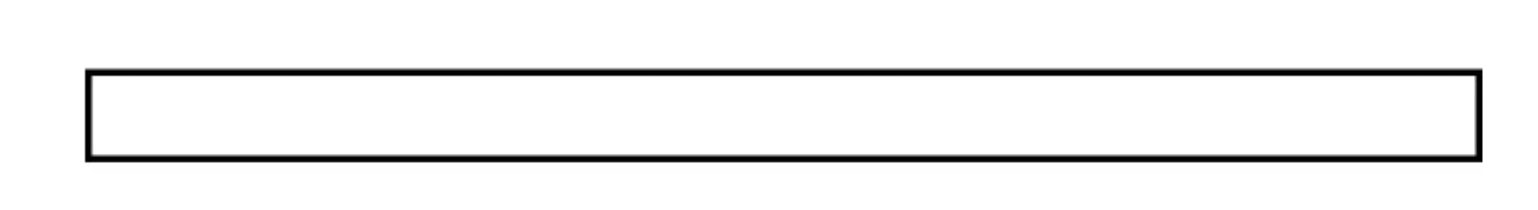
\includegraphics[scale=0.12]{naked_disk}
    \end{center}
    \item Formattazione fisica: il disco viene suddiviso in settori con le identificazioni e viene aggiunt
    lo spazio per la correzione di errori (ECC). 
    \begin{center} 
        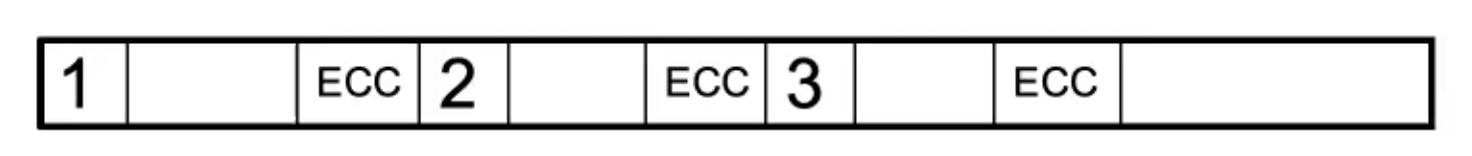
\includegraphics[scale=0.12]{format_physical_disk}
    \end{center}
    \item Formattazione logica: viene inserito il file system. Vengono create le strutture dati che 
    contengono una lista di spazio occupato (FAT), e di quello libero (FL - Free List) e directory vuote.
    \begin{center}
        \includegraphics[scale=0.12]{format_logical_disk}
    \end{center}
\end{itemize}

\subsection{Gestione dei blocchi difettosi}

ECC (\emph{Error Correction Code}) serve a capire, in lettura o scrittura, se un settore contiene dati 
corretti o meno. Lo schema tipico, ad esempio in lettura:
\begin{itemize}
    \item Il controllore legge un settore (incluso ECC)
    \item Il controllore calcola l'ECC per i dati appena letti
    \item Se il risultato \`e diverso $\Rightarrow$ Errore \emph{bad block}.
\end{itemize}

L'errore va segnalato, in modo che la parte di disco danneggiata non venga utilizzata in scrittura, altrimenti
non sarebbe pi\`u possibile leggere i dati. Per gestire i bad block esistono due modalit\`a: Off-line e On-line.

\subsubsection{Gestione off-line dei bad block}
Durante la formattazione logica si individuano i bad block e si mettono in una lista e vengono rimossi dai blocchi
disponibili. Avviene anche una marcatura della entry nella FAT.

Successivamente si puossono eseguire delle opportune utility per \emph{isolare} bad block (es. \texttt{CHKDSK} del DOS).
Questa tecnica di gestione \`e tipica dei controllori IDE. 

\subsubsection{gestione on-line dei bad block}
Il controllore si fa parte attiva ed \`e in grado di accorgersi se un blocco \`e danneggiato. Senza coinvolgere
il sistema operativo, il controllore del disco rimappa il bad block su un blocco buono, che dev'essere libero. 
Affinch\'e questa tecnica funzioni \`e necessario disporre di blocchi "di scorta" opportunamente riservati (\emph{sector sparing}).

Quando il sistema operativo richiede il bad block, il controllore mappa in modo trasparente l'accesso al bad
block sul blocco di scorta. 

Questa soluzione potrebbe inficiare le ottimizzazioni fornite dallo scheduling; per evitare ci\`o si 
allocano spare block in ogni cilindro.

\subsection{Gestione dello spazio di swap}

Lo spazio di swap viene usato dalla memoria virtuale come estensione della RAM. \`E possibile ricavarlo
dal normale file system, utilizzando comuni primitive di accesso a file. Questa tecnica \`e inefficiente
perch\'e il costo addizionale nell'attraversamento delle strutture dati per le directory e i file. 

L'opzione migliore \`e quella di posizionare l'area di swap in una partizione separata, che non contenga informazioni
o strutture relative al file system. L'accesso viene gestito usando uno speciale gestore dell'area di swap 
(\emph{swap daemon}).

% Riferimento: lezione del 15/05/2023
\chapter{File System}
























\end{document}
